\documentclass{natourDoc}
\usepackage{lipsum}
\usepackage{tabularx}
%\usepackage[table]{xcolor}
\usepackage{multirow}
\usepackage{svg}
\usepackage{amsmath}
\usepackage{pdfpages}
%\usepackage{placeins}
%\usepackage[T1]{fontenc}
\usepackage{ltablex}
\usepackage{longtable}
\usepackage{graphicx}
\usepackage{chngpage}
%\usepackage{hyperref}
\usepackage[dvipsnames]{xcolor}
\usepackage{listings}
\lstset{
    numbers=left,
    breaklines=true,
    tabsize=2,
    basicstyle=\ttfamily,
}

\lstdefinelanguage{Kotlin}{
  comment=[l]{//},
  commentstyle={\color{gray}\ttfamily},
  emph={filter, first, firstOrNull, forEach, lazy, map, mapNotNull, println},
  emphstyle={\color{OrangeRed}},
  identifierstyle=\color{black},
  keywords={!in, !is, abstract, actual, annotation, as, as?, break, by, catch, class, companion, const, constructor, continue, crossinline, data, delegate, do, dynamic, else, enum, expect, external, false, field, file, final, finally, for, fun, get, if, import, in, infix, init, inline, inner, interface, internal, is, lateinit, noinline, null, object, open, operator, out, override, package, param, private, property, protected, public, receiveris, reified, return, return@, sealed, set, setparam, super, suspend, tailrec, this, throw, true, try, typealias, typeof, val, var, vararg, when, where, while},
  keywordstyle={\color{NavyBlue}\bfseries},
  morecomment=[s]{/*}{*/},
  morestring=[b]",
  morestring=[s]{"""*}{*"""},
  ndkeywords={@RunWith, @InjectMocks, @Mock, @Before, @Test, @Deprecated, @JvmField, @JvmName, @JvmOverloads, @JvmStatic, @JvmSynthetic, Array, Byte, Double, Float, Int, Integer, Iterable, Long, Runnable, Short, String, Any, Unit, Nothing},
  ndkeywordstyle={\color{BurntOrange}\bfseries},
  sensitive=true,
  stringstyle={\color{ForestGreen}\ttfamily},
}

\hypersetup{
    colorlinks=true,
    linkcolor=black,
    filecolor=magenta,
    urlcolor=blue,
}

%\newcolumntype{a}{>{\columncolor{PineGreen!70}}l}

\def\arraystretch{1.5}

\title{Documentazione IngSW} %Titolo

\makeglossaries

\newglossaryentry{UX}
{
    name=UX,
    description={Termine utilizzato per definire la relazione tra una persona e un prodotto, un servizio, o un sistema. 
	Il termine presuppone un approccio olistico: cerca di comprendere tutto ciò che ruota attorno all'interazione di un utente con un prodotto}
}

\newglossaryentry{JWT}
{
    name=JWT,
    description={JSON Web Token - standard Internet proposto per la creazione di dati con firma opzionale e/o crittografia 
	opzionale il cui payload contiene JSON che asserisce un certo numero di attestazioni. I token 
	vengono firmati utilizzando un segreto privato o una chiave pubblica/privata}
}

\newglossaryentry{CASE}
{
    name=CASE,
    description={Gli strumenti C.A.S.E. (acronimo di Computer-Aided Software Engineering, ovvero sviluppo 
	del software assistito dal computer) sono quelli che supportano lo sviluppo del software attraverso interfacce grafiche (shell) e visuali e librerie di funzionalità}
}

\newglossaryentry{UI Design System}
{
    name=UI Design System,
    description={Raccolta di componenti che possono essere assemblati insieme 
	per costruire applicazioni e siti web. Il Design System permette ai team di progettazione e di sviluppo di costruire prodotti migliori e in modo più veloce, grazie alla possibilità di creare design riusabile e quindi scalabile}
}

\newglossaryentry{use-case driven}
{
    name=Use-case driven,
    description={Tecnica di modellazione nel processo di analisi dello sviluppo software. 
	Rende l'architettura del sistema modellata sulle esigenze degli utenti}
}

\newglossaryentry{deploy}
{
    name=Deploy,
    description={Distribuzione o rilascio al cliente, con relativa installazione, configurazione e messa in funzione o esercizio, di una applicazione o di un sistema software}
}

\newglossaryentry{REST}
{
    name=REST,
    description={L'acronimo REST sta per "Representational State Transfer" e si riferisce a uno stile architetturale 
	per sistemi distruibuiti. Rappresenta un sistema di trasmissione di dati basato su HTTP}
}

\newglossaryentry{UDF}
{
    name=UDF,
    description={L'acronimo UDF (Unidirectional Data Flow) è un design pattern dove gli stati fluiscono verso le componenti 
	inferiori e gli eventi verso quelle superiori}
}

\newglossaryentry{framework}
{
    name=Framework,
    description={Architettura logica di supporto sul quale un software può essere progettato e realizzato, spesso facilitandone lo sviluppo da parte del programmatore}
}

\newglossaryentry{open-source}
{
    name=Open-source,
    description={Tipo di software libero da vincoli di copyright o di altra natura}
}

\newglossaryentry{Mockito}
{
    name=Mockito,
    description={Framework di testing open source per Java. 
	Permette la creazione di oggetti test double in unit test automatizzati}
}

\newglossaryentry{WECT}
{
    name=WECT,
    description={Weak Equivalence Class Testing}
}

\newglossaryentry{CFG}
{
    name=CFG,
    description={Control Flow Graph}
}

\begin{document}

%----------- Informazioni --------------------

\titolo{Specifica, progettazione, implementazione e validazione del Sistema Informativo\\ \textit{NaTour21}} %Titolo.pdf
\sottotitolo{Dipartimento di Ingegneria Elettrica \\ e delle Tecnologie dell'Informazione} %Nome progetto

\professors{Sergio    \textsc{Di Martino} \\
	Francesco \textsc{Cutugno}
} %Nome docenti

\students{Bianca Giada \textsc{Chehade} N86003209 \\
	Mario 	   \textsc{Liguori} N86003258 \\
	Mattia 	   \textsc{Rossi} 	N86003211
} %Nome studenti

%----------- Inizializzazione -----------------

\marginscreate %Crea margini
\cover %Crea cover
\toc %Crea Table of Contents

%------------ Corpo del documento ----------------
\newpage
\section{Documento dei Requisiti Software}
\subsection{Descrizione del progetto}
NaTour21 è un sistema complesso e distribuito finalizzato ad offrire un moderno social network multipiattaforma per appassionati di escursioni.\\

Il sistema consiste in:
\begin{itemize}
	\item un Back-End sicuro, performante e scalabile;
	\item un client mobile attraverso cui gli
	      utenti possono fruire delle funzionalità del sistema in modo intuitivo, rapido e piacevole;
	\item un client mobile attraverso cui gli amministratori possono gestire i contenuti inseriti in piattaforma.\\
\end{itemize}

NaTour21 ha lo scopo di creare una community sicura e affidabile dove condividere la propria passione per l'escursionismo.\\

In questo scenario, l'utente si configura come protagonista: oltre alla possibilità di inserire itinerari (dettagliati da informazioni), compilation e post personali sulla piattaforma,
è lasciato ampio spazio all'individualità personale.\\

Tutto ciò si concretizza con la possibilità di interagire con gli altri utenti, in modo da poter avere un contatto più diretto con
la realtà dell'escursionismo, e di lasciare valutazioni personali su qualunque itinerario si desideri.\\

Il sistema valuta essenziale la sicurezza degli utenti: questi potranno segnalare informazioni inesatte o contenuti inappropriati al fine
di rendere la permanenza nella community piacevole per tutti.

\subsection{Presentazione dell'idea progettuale}

L'applicazione \textbf{NaTour21} nasce in seguito all'esigenza di uno spazio virtuale dove poter condividere la passione per l'escursionismo.\\
Creare una community di escursionisti, esperti o meno, ha lo scopo di rendere le esperienze individuali degli utenti più sicure e informate,
oltre a promuovere la condivisione di contenuti personali.\\\\
NaTour21 mette a disposizione degli utenti registrati diverse funzionalità.\\
Il lato prettamente informativo consente di ricercare - nonchè inserire in piattaforma - diversi itinerari, e tutte le informazioni relative ad essi.
Ciò comprende la possibilità di visualizzarli su mappa, e, per garantire un'accuratezza maggiore delle informazioni, di lasciare
un feedback personale per ciascuno di essi.\\\\
Ci sono, però, ulteriori funzionalità che coinvolgono direttamente l'utente: tra queste la condivisione di post, la creazione di compilation personalizzate e
la visualizzazione di una homepage con post riguardanti diversi itinerari.\\
Particolare attenzione è riservata alla sicurezza degli utenti, i quali possono segnalare contenuti inappropriati o informazioni inesatte.

\subsection{Individuazione del target degli utenti}
NaTour21 si configura come community in cui chiunque può intraprendere la passione per l'escursionismo e condividerla.\\
Ciononostante, è stato possibile individuare un target di utenti ben definito grazie ai dati
statistici\footnote{Fonte: \href{http://dati.istat.it/Index.aspx?DataSetCode=DCCV_ESC_CAPI}{sito ufficiale Istat}.} raccolti
nell'anno 2020 dall'ISTAT, Istituto Nazionale di Statistica.\\\\
In seguito all'analisi delle informazioni statistiche sull'escursionismo italiano è stato individuato come target utenti la popolazione, caratterizzata da un
numero di circa pari entità di uomini e di donne, nella fascia di età \texttt{35-64}. La maggior parte della
platea considerata risulta essere appartenente alla condizione lavorativa di \textit{dirigente, quadro o impiegato}.\\\\
\begin{figure}[!htbp]
	\centering
	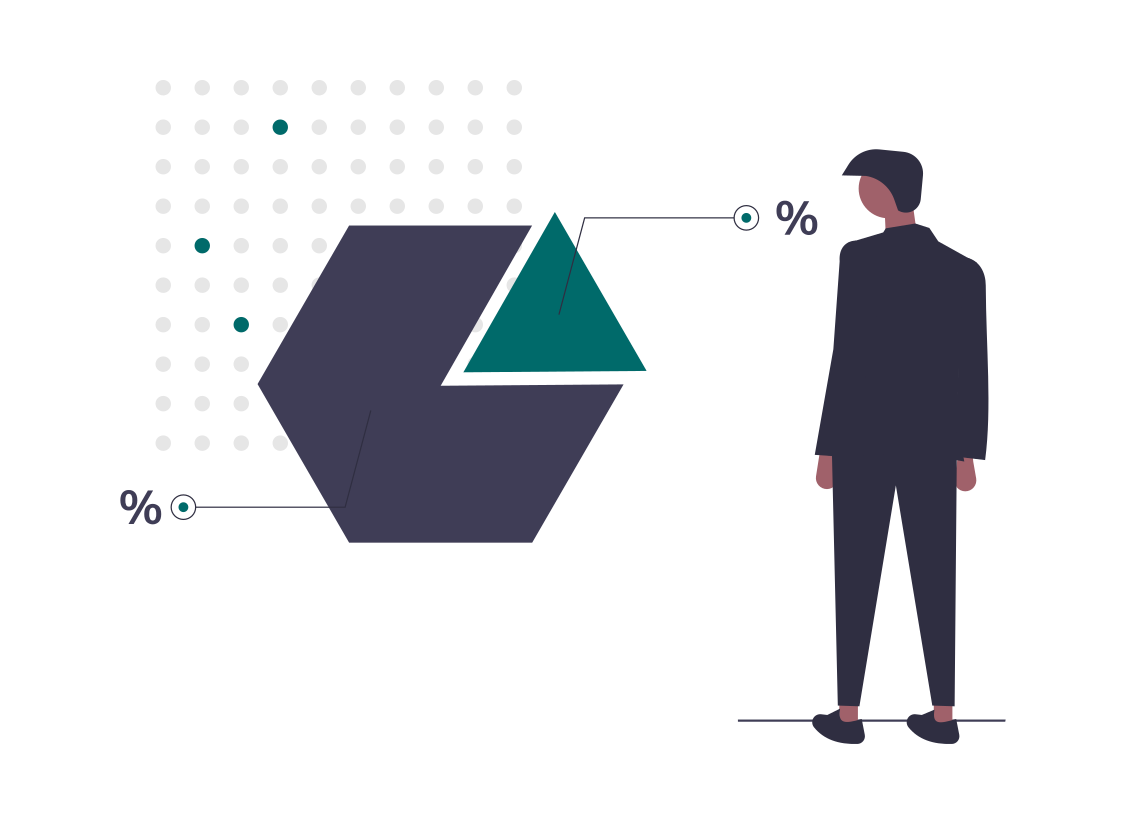
\includegraphics[width=12cm, page=1]{./logos/undraw_statistic_chart_38b6.png}
\end{figure}
\FloatBarrier
L'Istat ha inoltre conteggiato nell'anno 2020 circa \texttt{41194} escursioni giornaliere,
di cui il \texttt{42.7\%} situate temporalmente nel terzo trimestre dell'anno. Da questa informazione si deduce che il periodo
preferito per attività escursionistiche sia quello dei mesi estivi.\\\\
Il motivo prevalente per queste escursioni risulta essere stato \textit{piacere personale, svago e tempo libero}, con un numero
di escursioni così orientate pari a \texttt{23223}: questo dato risulta particolarmente significativo, pari a un ordine
di grandezza in più rispetto agli altri motivi registrati. È importante anche notare quanto il numero di escursioni in paesi
esteri sia di gran lunga minore rispetto a quelle nelle regioni italiane.\\\\
Le regioni del Nord Italia sembrano essere state le preferite per visite giornaliere (la più visitata è stata il Veneto, con una media di
\texttt{6200}), seguite immediatamente da quelle del centro-Sud. Il Molise, invece, non risulta aver raggiunto
la minima cifra considerata nella raccolta dati.\\

\subsection{Requisiti funzionali}
In questa sezione saranno esposti i requisiti \textit{funzionali} dell'applicazione NaTour21, cioè le funzionalità offerte.
Le funzionalità richieste sono presenti nella loro totalità; inoltre, è stato ritenuto opportuno inserire alcune funzionalità non
esplicitamente richieste, ma ritenute dal team di sviluppo come desiderabili per qualsiasi applicativo di questo tipo.

\subsubsection{Autenticazione}
\begin{table}[H]
	\centering
	\begin{tabular}{ |p{5cm}|p{10.3cm}| }
		\hline
		\rowcolor{PineGreen!70}
		\textbf{Nome} & \textbf{Descrizione}                                                                                                                                               \\
		\hline
		Registrazione & Il sistema deve consentire a un utente di potersi registrare indicando e-mail, username e password, oppure utilizzando account di terze parti (Google o Facebook). \\
		\hline
	\end{tabular}
	\caption{RF.1}
\end{table}

\begin{table}[H]
	\centering
	\begin{tabular}{ |p{5cm}|p{10.3cm}| }
		\hline
		\rowcolor{PineGreen!70}
		\textbf{Nome} & \textbf{Descrizione}                                                                                                                                 \\
		\hline
		Accesso       & Il sistema deve consentire a un utente registrato di poter effettuare l'accesso alla piattaforma avendo eseguito precendentemente una registrazione. \\
		\hline
	\end{tabular}
	\caption{RF.2}

\end{table}

\begin{table}[H]
	\centering
	\begin{tabular}{ |p{5cm}|p{10.3cm}| }
		\hline
		\rowcolor{PineGreen!70}
		\textbf{Nome}           & \textbf{Descrizione}                                                                                               \\
		\hline
		Reimpostazione password & Il sistema deve consentire a un utente registrato di poter reimpostare la propria password se dimenticata o persa. \\
		\hline
	\end{tabular}
	\caption{RF.3}

\end{table}

\begin{table}[H]
	\centering
	\begin{tabular}{ |p{5cm}|p{10.3cm}| }
		\hline
		\rowcolor{PineGreen!70}
		\textbf{Nome}       & \textbf{Descrizione}                                                                                                \\
		\hline
		Uscita dall'account & Il sistema deve consentire a un utente autenticato di poter uscire dall'account con il quale ha eseguito l'accesso. \\
		\hline
	\end{tabular}
	\caption{RF.4}

\end{table}


\subsubsection{Interazione con un itinerario}
\begin{table}[H]
	\centering
	\begin{tabular}{ |p{5cm}|p{10.3cm}| }
		\hline
		\rowcolor{PineGreen!70}
		\textbf{Nome}             & \textbf{Descrizione}                                                    \\
		\hline
		Visualizzazione itinerari & Il sistema deve consentire a un utente autenticato di visualizzare i
		dettagli degli itinerari pubblicati (tra cui la sua posizione su mappa) e i post ad essi associati. \\
		\hline
	\end{tabular}
	\caption{RF.5}

\end{table}

\begin{table}[H]
	\centering
	\begin{tabular}{ |p{5cm}|p{10.3cm}| }
		\hline
		\rowcolor{PineGreen!70}
		\textbf{Nome}          & \textbf{Descrizione}                                                                                                    \\
		\hline
		Inserimento itinerario & Il sistema deve consentire a un utente autenticato di inserire nuovi itinerari (sentieri) in piattaforma. Un sentiero è
		caratterizzato da un nome, una durata (max 16 ore), un livello di difficoltà, un punto di inizio e di fine, delle foto (max 5), una descrizione
		(opzionale), e un tracciato geografico (opzionale) che lo rappresenta su una mappa. Il tracciato
		geografico può essere inseribile manualmente (interagendo con una mappa interattiva) oppure
		tramite file in formato standard GPX.                                                                                                            \\
		\hline
	\end{tabular}
	\caption{RF.6}

\end{table}

\begin{table}[H]
	\centering
	\begin{tabular}{ |p{5cm}|p{10.3cm}| }
		\hline
		\rowcolor{PineGreen!70}
		\textbf{Nome}     & \textbf{Descrizione}                                                                                                                                               \\
		\hline
		Ricerca itinerari & Il sistema deve consentire a un utente autenticato di effettuare ricerche di itinerari tra quelli presenti in piattaforma, con possibilità di filtrare i risultati
		per area geografica (compresa in un raggio espresso in km scelto dall'utente), per livello di difficoltà, per durata e per accessibilità ai disabili.                                  \\
		\hline
	\end{tabular}
	\caption{RF.7}

\end{table}

\begin{table}[H]
	\centering
	\begin{tabular}{ |p{5cm}|p{10.3cm}| }
		\hline
		\rowcolor{PineGreen!70}
		\textbf{Nome}          & \textbf{Descrizione}                                                                                   \\
		\hline
		Valutazione itinerario & Il sistema deve consentire a un utente autenticato di indicare un punteggio di difficoltà e/o un tempo
		di percorrenza diverso da quello indicato dall’utente che ha inserito il sentiero. In questo caso, il
		punteggio di difficoltà e il tempo di percorrenza per il sentiero saranno ri-calcolati come la media
		delle difficoltà e dei tempi indicati.                                                                                          \\
		\hline
	\end{tabular}
	\caption{RF.8}

\end{table}

\begin{table}[H]
	\centering
	\begin{tabular}{ |p{5cm}|p{10.3cm}| }
		\hline
		\rowcolor{PineGreen!70}
		\textbf{Nome}          & \textbf{Descrizione}                                                        \\
		\hline
		Salvataggio itinerario & Il sistema deve consentire a un utente autenticato di salvare gli itinerari
		nelle proprie compilation personalizzate.                                                            \\
		\hline
	\end{tabular}
	\caption{RF.9}

\end{table}

\begin{table}[H]
	\centering
	\begin{tabular}{ |p{5cm}|p{10.3cm}| }
		\hline
		\rowcolor{PineGreen!70}
		\textbf{Nome}           & \textbf{Descrizione}                                                            \\
		\hline
		Segnalazione itinerario & Il sistema deve consentire a un utente autenticato di segnalare degli itinerari
		le quali informazioni potrebbero non essere corrette e/o aggiornate.                                      \\
		\hline
	\end{tabular}
	\caption{RF.10}

\end{table}

\begin{table}[H]
	\centering
	\begin{tabular}{ |p{5cm}|p{10.3cm}| }
		\hline
		\rowcolor{PineGreen!70}
		\textbf{Nome}        & \textbf{Descrizione}                                                             \\
		\hline
		Rimozione itinerario & Il sistema deve consentire a un utente autenticato di eliminare itinerari di cui
		è l'autore.                                                                                             \\
		\hline
	\end{tabular}
	\caption{RF.11}

\end{table}

\subsubsection{Interazione con un post}
\begin{table}[H]
	\centering
	\begin{tabular}{ |p{5cm}|p{10.3cm}| }
		\hline
		\rowcolor{PineGreen!70}
		\textbf{Nome}        & \textbf{Descrizione}                                               \\
		\hline
		Visualizzazione post & Il sistema deve consentire a un utente autenticato di visualizzare
		i dettagli di un post.                                                                    \\
		\hline
	\end{tabular}
	\caption{RF.12}

\end{table}

\begin{table}[H]
	\centering
	\begin{tabular}{ |p{5cm}|p{10.3cm}| }
		\hline
		\rowcolor{PineGreen!70}
		\textbf{Nome}    & \textbf{Descrizione}                                                                               \\
		\hline
		Inserimento post & Il sistema deve consentire a un utente autenticato di inserire un post associato ad un itinerario,
		caratterizzato da foto (max 5) e una descrizione (opzionale).                                                         \\
		\hline
	\end{tabular}
	\caption{RF.13}

\end{table}


\begin{table}[H]
	\centering
	\begin{tabular}{ |p{5cm}|p{10.3cm}| }
		\hline
		\rowcolor{PineGreen!70}
		\textbf{Nome}     & \textbf{Descrizione}                                                                \\
		\hline
		Segnalazione post & Il sistema deve consentire a un utente autenticato di segnalare post con fotografie
		inappropriate.                                                                                          \\
		\hline
	\end{tabular}
	\caption{RF.14}

\end{table}

\begin{table}[H]
	\centering
	\begin{tabular}{ |p{5cm}|p{10.3cm}| }
		\hline
		\rowcolor{PineGreen!70}
		\textbf{Nome}  & \textbf{Descrizione}                                                        \\
		\hline
		Rimozione post & Il sistema deve consentire a un utente autenticato di eliminare post di cui
		è l'autore.                                                                                  \\
		\hline
	\end{tabular}
	\caption{RF.15}

\end{table}

\subsubsection{Gestione dati personali e conversazioni private}
\begin{table}[H]
	\centering
	\begin{tabular}{ |p{5cm}|p{10.3cm}| }
		\hline
		\rowcolor{PineGreen!70}
		\textbf{Nome}    & \textbf{Descrizione}                                                                    \\
		\hline
		Gestione profilo & Il sistema deve consentire a un utente autenticato di gestire il suo profilo,
		quindi di visualizzare i contenuti inseriti ed eliminarli. Inoltre è possibile modificare la foto profilo. \\
		\hline
	\end{tabular}
	\caption{RF.16}

\end{table}

\begin{table}[H]
	\centering
	\begin{tabular}{ |p{5cm}|p{10.3cm}| }
		\hline
		\rowcolor{PineGreen!70}
		\textbf{Nome}                  & \textbf{Descrizione}                                                                            \\
		\hline
		Gestione conversazioni private & Il sistema deve consentire a un utente autenticato lo scambio di informazioni con altri utenti.
		È possibile avviare la conversazione a partire dai contenuti pubblicati. Inoltre è possibile ricercare un destinatario.          \\
		\hline
	\end{tabular}
	\caption{RF.17}

\end{table}

\subsubsection{Interazione con una compilation}
\begin{table}[H]
	\centering
	\begin{tabular}{ |p{5cm}|p{10.3cm}| }
		\hline
		\rowcolor{PineGreen!70}
		\textbf{Nome}         & \textbf{Descrizione}                                                                                    \\
		\hline
		Creazione compilation & Il sistema deve consentire a un utente autenticato di creare delle \textit{compilation personalizzate},
		caratterizzate da un titolo, una foto e da una descrizione.                                                                     \\
		\hline
	\end{tabular}
	\caption{RF.18}

\end{table}

\begin{table}[H]
	\centering
	\begin{tabular}{ |p{5cm}|p{10.3cm}| }
		\hline
		\rowcolor{PineGreen!70}
		\textbf{Nome}         & \textbf{Descrizione}                                                       \\
		\hline
		Rimozione compilation & Il sistema deve consentire a un utente autenticato di eliminare le proprie
		compilation personalizzate.                                                                        \\
		\hline
	\end{tabular}
	\caption{RF.19}

\end{table}

\begin{table}[H]
	\centering
	\begin{tabular}{ |p{5cm}|p{10.3cm}| }
		\hline
		\rowcolor{PineGreen!70}
		\textbf{Nome}               & \textbf{Descrizione}                                                          \\
		\hline
		Visualizzazione compilation & Il sistema deve consentire a un utente autenticato di visualizzare i dettagli
		delle proprie compilation.                                                                                  \\
		\hline
	\end{tabular}
	\caption{RF.20}

\end{table}


\begin{table}[H]
	\centering
	\begin{tabular}{ |p{5cm}|p{10.3cm}| }
		\hline
		\rowcolor{PineGreen!70}
		\textbf{Nome}                       & \textbf{Descrizione}                                                          \\
		\hline
		Rimozione itinerario da compilation & Il sistema deve consentire a un utente autenticato di rimuovere gli itinerari
		dalle proprie compilation personalizzate.                                                                           \\
		\hline
	\end{tabular}
	\caption{RF.21}

\end{table}

\subsubsection{Requisiti amministratore}
Il seguente insieme di funzionalità è ridotto ad un gruppo ristretto di utenti: gli amministratori.\footnote{È importante sottolineare che un amministratore è un utente semplice con particolari privilegi:
	un amministratore potrà, dunque, usufruire di tutte le funzionalità riservate agli
	utenti. Non vale, però, il viceversa: gli utenti "semplici" non avranno alcun potere
	sui contenuti pubblicati da altri utenti, se non la possibilità di segnalarli agli
	amministratori.}

\begin{table}[H]
	\centering
	\begin{tabular}{ |p{5cm}|p{10.3cm}| }
		\hline
		\rowcolor{PineGreen!70}
		\textbf{Nome}                & \textbf{Descrizione}                                                                                 \\
		\hline
		Visualizzazione segnalazioni & Il sistema deve consentire a un utente autenticato con i privilegi di amministratore di visualizzare
		la lista di segnalazioni inviate.                                                                                                   \\
		\hline
	\end{tabular}
	\caption{RF.22}

\end{table}

\begin{table}[H]
	\centering
	\begin{tabular}{ |p{5cm}|p{10.3cm}| }
		\hline
		\rowcolor{PineGreen!70}
		\textbf{Nome}              & \textbf{Descrizione}                                                                                 \\
		\hline
		Amministrazione itinerario & Il sistema deve consentire a un utente autenticato con i privilegi di amministratore di modificare o
		rimuovere un itinerario segnalato.                                                                                                \\
		\hline
	\end{tabular}
	\caption{RF.23}
\end{table}

\newpage
\subsection{Requisiti non funzionali}
Questa sezione conterrà invece i requisiti \textit{non funzionali} dell'applicazione, ovvero tutti i vincoli sui servizi offerti dal sistema.

\begin{table}[H]
	\centering
	\begin{tabular}{ |p{5cm}|p{10.3cm}| }
		\hline
		\rowcolor{PineGreen!70}
		\textbf{Nome}      & \textbf{Descrizione}                                                                 \\
		\hline
		Back-End scalabile & Il sistema deve essere scalabile e performante rispetto ai cambiamenti del Back-End,
		in modo da garantire un'agile manutenibilità nel tempo.                                                   \\
		\hline
	\end{tabular}
	\caption{RNF1}
\end{table}

\begin{table}[H]
	\centering
	\begin{tabular}{ |p{5cm}|p{10.3cm}| }
		\hline
		\rowcolor{PineGreen!70}
		\textbf{Nome} & \textbf{Descrizione}                                                                           \\
		\hline
		Prestazioni   & Il sistema deve essere operativo entro 3 secondi dall'avvio e, inoltre, non deve ostacolare in
		alcun modo gli input dell'utente (e.g. presentando dei rallentamenti).                                         \\
		\hline
	\end{tabular}
	\caption{RNF2}
\end{table}

\begin{table}[H]
	\centering
	\begin{tabular}{ |p{5cm}|p{10.3cm}| }
		\hline
		\rowcolor{PineGreen!70}
		\textbf{Nome} & \textbf{Descrizione}                                                                                             \\
		\hline
		Reattività    & Il sistema deve essere responsivo, sia nei confronti degli input da parte dell'utente, sia
		in caso di interruzioni esterne con alta priorità (e.g. chiamate in arrivo).
		Considerando il caso delle interruzioni: il sistema deve essere in grado di salvare il proprio stato e ripresentarlo all'utente. \\
		\hline
	\end{tabular}
	\caption{RNF3}
\end{table}

\begin{table}[H]
	\centering
	\begin{tabular}{ |p{5cm}|p{10.3cm}| }
		\hline
		\rowcolor{PineGreen!70}
		\textbf{Nome} & \textbf{Descrizione}                                                                          \\
		\hline
		Usabilità     & L'applicazione deve presentare una \Gls{UX} semplice, che renda il flusso delle operazioni
		comprensibile anche ad utenti meno esperti.                                                                   \\
		\hline
	\end{tabular}
	\caption{RNF4}
\end{table}

\begin{table}[H]
	\centering
	\begin{tabular}{ |p{5cm}|p{10.3cm}| }
		\hline
		\rowcolor{PineGreen!70}
		\textbf{Nome} & \textbf{Descrizione}                                                                              \\
		\hline
		Sicurezza     & Il sistema deve essere sicuro, con dati criptati e protetti da attacchi esterni.
		Nel caso dell'autenticazione per i client, verrà salvato un token (nello specifico \Gls{JWT}) sul dispositivo. \\
		\hline
	\end{tabular}
	\caption{RNF5}
\end{table}

\begin{table}[H]
	\centering
	\begin{tabular}{ |p{5cm}|p{10.3cm}| }
		\hline
		\rowcolor{PineGreen!70}
		\textbf{Nome}      & \textbf{Descrizione}                                                   \\
		\hline
		Sicurezza password & Il sistema non deve consentire di inserire password che non contengano
		almeno 8 caratteri.                                                                         \\
		\hline
	\end{tabular}
	\caption{RNF6}
\end{table}

\begin{table}[H]
	\centering
	\begin{tabular}{ |p{5cm}|p{10.3cm}| }
		\hline
		\rowcolor{PineGreen!70}
		\textbf{Nome}          & \textbf{Descrizione}                                                            \\
		\hline
		Numero massimo di foto & Il sistema non deve consentire di inserire più di 5 foto per itinerario o post. \\
		\hline
	\end{tabular}
	\caption{RNF7}
\end{table}

\newpage
\subsection{Requisiti di dominio}
Infine, questa sezione conterrà i requisiti \textit{di dominio} dell'applicazione, ovvero tutti i vincoli generali a cui l'applicativo
deve attenersi. \\

\begin{table}[H]
	\centering
	\begin{tabular}{ |p{5cm}|p{10.3cm}| }
		\hline
		\rowcolor{PineGreen!70}
		\textbf{Nome}      & \textbf{Descrizione}                                              \\
		\hline
		ISO/IEC 27018:2019 & Il sistema deve essere conforme allo standard ISO/IEC 27018:2019,
		incentrato sulla protezione dei dati personali nel cloud.                              \\
		\hline
	\end{tabular}
	\caption{RD1}

\end{table}

\begin{table}[H]
	\centering
	\begin{tabular}{ |p{5cm}|p{10.3cm}| }
		\hline
		\rowcolor{PineGreen!70}
		\textbf{Nome} & \textbf{Descrizione}                                                                      \\
		\hline
		GDPR          & Il sistema deve essere conforme al GDPR (Regolamento Generale sulla Protezione dei Dati),
		incentrato sul trattamento dei dati personali e sulla privacy dell’utente.                                \\
		\hline
	\end{tabular}
	\caption{RD2}

\end{table}

\newpage

\newpage
\subsection{Modellazione dei Casi d'Uso}
In questa sezione è riportato il diagramma Use Case per l'applicazione.\\
Per garantire una maggiore leggibilità e data la molteplicità di funzioni garantite
dal sistema, si è fatta la scelta di raggruppare le funzioni logicamente legate
tra loro in packages.

\begin{figure}[!htbp]
	\centering
	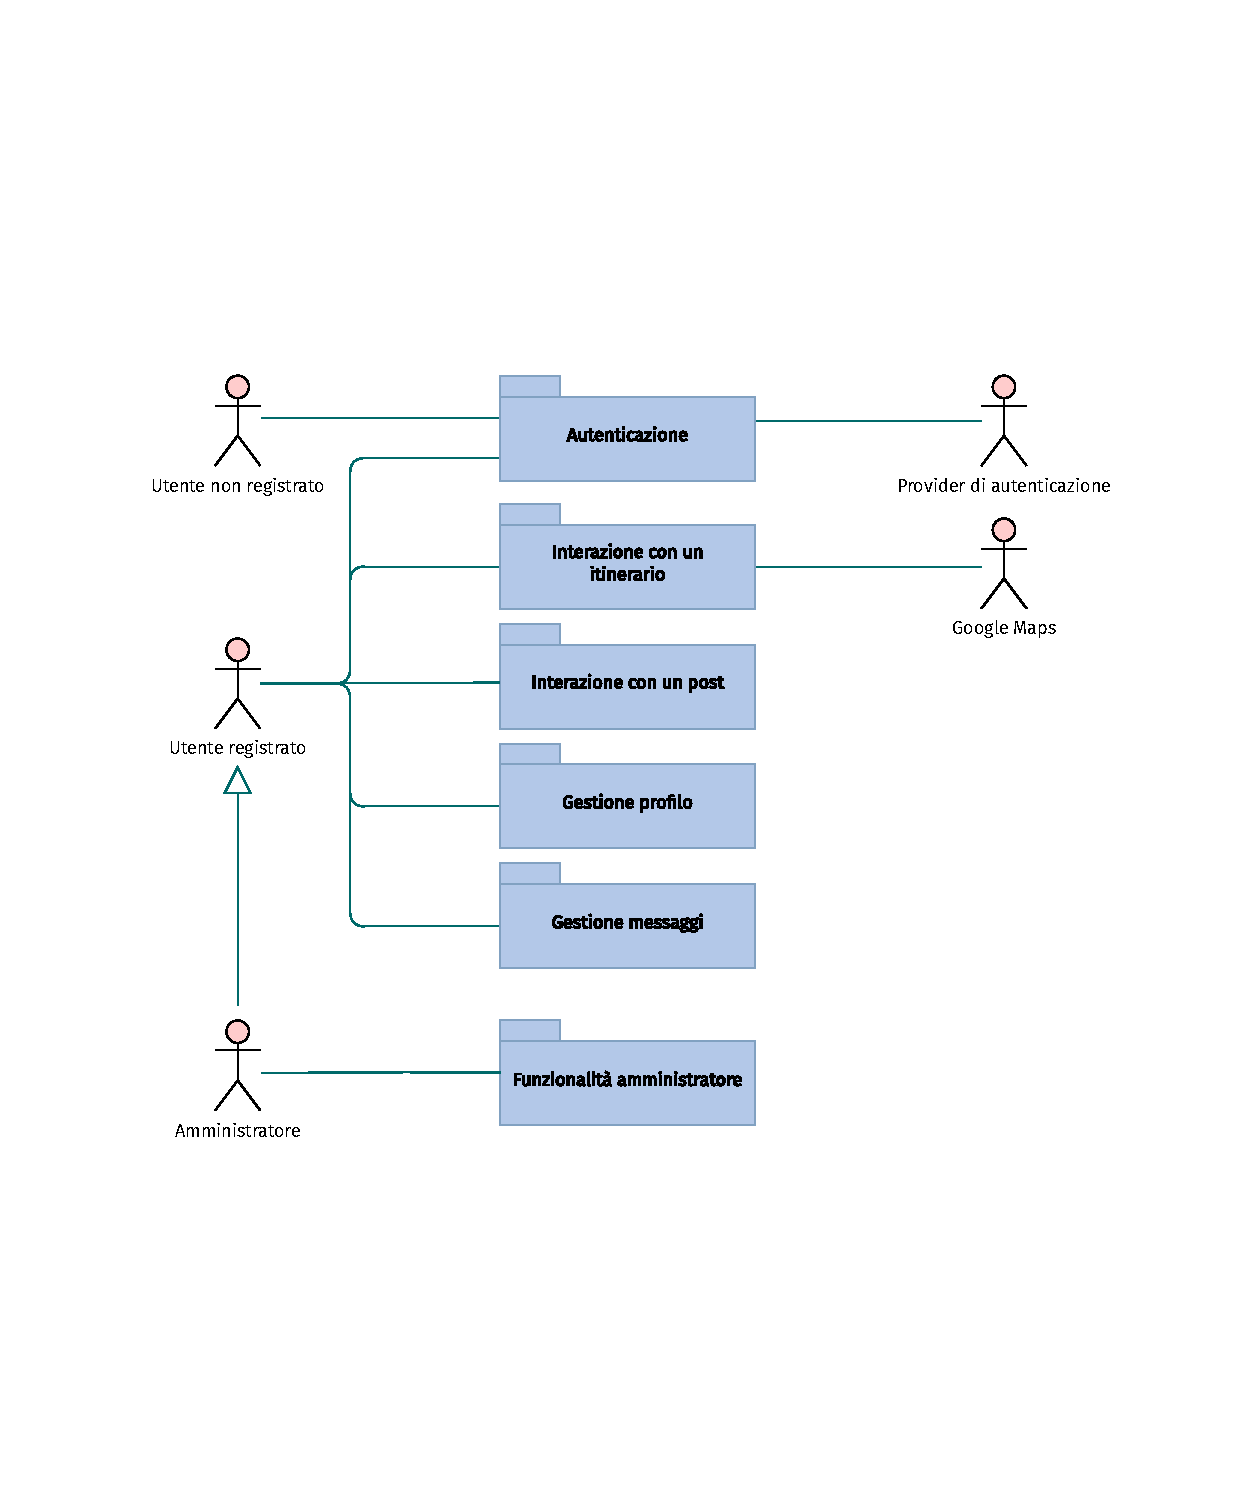
\includegraphics[width=\textwidth, page=1]{./diagrams/useCase.pdf}
	\caption{Use Case Diagram}
\end{figure}
\FloatBarrier

\newpage
\subsubsection{Autenticazione}
\begin{figure}[!htbp]
	\centering
	\includegraphics[width=\textwidth, page=2]{./diagrams/useCase.pdf}
	\caption{Package 1 - Autenticazione}
\end{figure}
\FloatBarrier

\newpage
\subsubsection{Interazione con un itinerario}
\begin{figure}[!htbp]
	\centering
	\includegraphics[width=\textwidth, page=3]{./diagrams/useCase.pdf}
	\caption{Package 2 - Interazione con un itinerario}
\end{figure}
\FloatBarrier

\newpage
\subsubsection{Interazione con un post}
\begin{figure}[!htbp]
	\centering
	\includegraphics[width=\textwidth, page=4]{./diagrams/useCase.pdf}
	\caption{Package 3 - Interazione con un post}
\end{figure}
\FloatBarrier

\newpage
\subsubsection{Gestione profilo}
\begin{figure}[!htbp]
	\centering
	\includegraphics[width=\textwidth, page=5]{./diagrams/useCase.pdf}
	\caption{Package 4 - Gestione profilo}
\end{figure}
\FloatBarrier

\newpage
\subsubsection{Gestione messaggi}
\begin{figure}[!htbp]
	\centering
	\includegraphics[width=\textwidth, page=6]{./diagrams/useCase.pdf}
	\caption{Package 5 - Gestione messaggi}
\end{figure}
\FloatBarrier

\newpage
\subsubsection{Funzionalità amministratore}
\begin{figure}[!htbp]
	\centering
	\includegraphics[width=\textwidth, page=7]{./diagrams/useCase.pdf}
	\caption{Package 6 - Funzionalità amministratore}
\end{figure}
\FloatBarrier

\newpage
\subsection{Tabelle di Cockburn dei casi d'uso}
Sono presentate in questa sezione le tabelle di Cockburn relative a due casi d'uso significativi dello Use Case Diagram.

\subsubsection{Inserisce un itinerario}

\def\arraystretch{1.5}
\begin{tabularx}{\linewidth}{| l | p{1cm} | p{4cm} | X | X|}
	\hline
	\rowcolor{PineGreen!70}
	\textbf{USE CASE \#1}         & \multicolumn{4} {l|}{\textbf{Inserisce un itinerario}}                                                                                                                                                                                                                                                                                                                                                                                                      \\
	\hline Goal in Context        & \multicolumn{4}{>{\hsize=\dimexpr 4\hsize+4\tabcolsep+2\arrayrulewidth\relax}X|}{L’utente vuole inserire un itinerario in piattaforma}                                                                                                                                                                                                                                                                                                                      \\

	\hline Preconditions          &
	\multicolumn{4}{l|}{L’utente è autenticato}                                                                                                                                                                                                                                                                                                                                                                                                                                                 \\

	\hline Success End Conditions &
	\multicolumn{4}{l|}{L’utente riesce ad inserire il nuovo itinerario}                                                                                                                                                                                                                                                                                                                                                                                                                        \\

	\hline Failed End Conditions  &
	\multicolumn{4}{l|}{L’utente non riesce ad inserire il nuovo itinerario}                                                                                                                                                                                                                                                                                                                                                                                                                    \\

	\hline Primary Actor          &
	\multicolumn{4}{l|}{Utente registrato}                                                                                                                                                                                                                                                                                                                                                                                                                                                      \\

	\hline Secondary Actor        &
	\multicolumn{4}{l|}{Google Maps}                                                                                                                                                                                                                                                                                                                                                                                                                                                            \\

	\hline Trigger                & \multicolumn{4}{>{\hsize=\dimexpr 4\hsize+4\tabcolsep+2\arrayrulewidth\relax}X|}{                                                                                                                                                                                                                                                                                                                                                                           %
	L’utente preme il Floating Action Button “Nuovo itinerario” nella schermata “RoutesUI”  }                                                                                                                                                                                                                                                                                                                                                                                                   \\

	\hline
	\multirow{2}{*}{}
	                              & Step                                                                                                                                   & Utente registrato                                                                                                                                                    & Sistema                                             & Google Maps                                                                           \\

	\cline{2-5}                   & 1                                                                                                                                      & Preme il Floating Action Button “Nuovo itinerario” nella schermata “RoutesUI”
	                              &                                                                                                                                        &                                                                                                                                                                                                                                                                                                                    \\

	\cline{2-5}                   & 2                                                                                                                                      &                                                                                                                                                                      & Mostra la schermata “CreateRouteInfoUI”             &                                                                                       \\

	\cline{2-5}                   & 3                                                                                                                                      & Inserisce il nome dell’itinerario, (opzionalmente) la descrizione, la durata approssimativa, il livello di difficoltà e la possibilità di accessibilità per disabili &                                                     &                                                                                       \\

	\cline{2-5}                   & 4                                                                                                                                      & Preme il Floating Action Button “nextFab”                                                                                                                            &                                                     &                                                                                       \\

	\cline{2-5}                   & 5                                                                                                                                      &                                                                                                                                                                      & Mostra la schermata “CreateRouteMapUI”              &                                                                                       \\

	\cline{2-5}                   & 6                                                                                                                                      & Preme sull’icona di ricerca                                                                                                                                          &                                                     &                                                                                       \\

	\cline{2-5}                   & 7                                                                                                                                      & Inserisce la posizione della prima tappa del percorso per visualizzarla sulla mappa                                                                                  &                                                     &                                                                                       \\

	\cline{2-5}                   & 8                                                                                                                                      &                                                                                                                                                                      &                                                     & Mostra la posizione desiderata sulla mappa                                            \\

	\cline{2-5}                   & 9                                                                                                                                      & Seleziona le tappe del percorso tramite la mappa interattiva                                                                                                         &                                                     & Recupera la posizione dei punti selezionati sulla mappa e traccia i percorsi tra essi \\

	\cline{2-5}                   & 10                                                                                                                                     & Preme il Floating Action Button “nextFab”                                                                                                                            &                                                     &                                                                                       \\

	\cline{2-5}                   & 11                                                                                                                                     &                                                                                                                                                                      & Mostra la schermata “CreateRoutePhotosUI”           &                                                                                       \\

	\cline{2-5}                   & 12                                                                                                                                     & Preme il bottone "Seleziona foto"                                                                                                                                    &                                                     &                                                                                       \\

	\cline{2-5}                   & 13                                                                                                                                     &                                                                                                                                                                      & Mostra il photo picker per la selezione delle foto  &                                                                                       \\

	\cline{2-5}                   & 14                                                                                                                                     & Seleziona un numero di foto compreso tra 1 e 5                                                                                                                       &                                                     &                                                                                       \\

	\cline{2-5}                   & 15                                                                                                                                     & Preme il bottone “Fatto”                                                                                                                                             &                                                     &                                                                                       \\

	\cline{2-5}                   & 16                                                                                                                                     &                                                                                                                                                                      & Mostra la schermata “CreateRoutePhotosUI”           &                                                                                       \\

	\cline{2-5}                   & 17                                                                                                                                     & Preme il Floating Action Button “Inserisci itinerario”                                                                                                               &                                                     &                                                                                       \\

	\hline
	\multirow{2}{*}{\shortstack[l]{EXTENSION \#1                                                                                                                                                                                                                                                                                                                                                                                                                                                \\ Inserimento mappa \\ con file GPX}}
	                              & Step                                                                                                                                   & Utente registrato                                                                                                                                                    & Sistema                                             & Google Maps                                                                           \\

	\cline{2-5}                   & 9.1                                                                                                                                    & Apre il menu a tendina in alto a destra della schermata e seleziona “Importa GPX”                                                                                    &                                                     &                                                                                       \\

	\cline{2-5}                   & 10.1                                                                                                                                   &                                                                                                                                                                      & Mostra la schermata per la selezione di un file GPX &                                                                                       \\

	\cline{2-5}                   & 11.1                                                                                                                                   & Seleziona il file GPX                                                                                                                                                &                                                     &                                                                                       \\

	\cline{2-5}                   & 12.1                                                                                                                                   &                                                                                                                                                                      & Mostra la schermata "CreateRouteMapUI" aggiornata   &                                                                                       \\

	\hline
\end{tabularx}

\newpage

\subsubsection{Segnala un itinerario}

\def\arraystretch{1.5}
\begin{tabularx}{\linewidth}{|l| p{1cm} | p{4cm} | X |}
	\hline
	\rowcolor{PineGreen!70}
	\textbf{USE CASE \#2}         & \multicolumn{3} {l|}{\textbf{Segnala un itinerario}}                                                                                                                                                                                  \\

	\hline
	Goal in Context               &
	\multicolumn{3}{>{\hsize=\dimexpr 3\hsize+3\tabcolsep+2\arrayrulewidth\relax}X|}
	{L’utente vuole segnalare un itinerario per informazioni inesatte o non accurate}                                                                                                                                                                                     \\

	\hline
	Preconditions                 &
	\multicolumn{3}{l|}{L’utente è autenticato}                                                                                                                                                                                                                           \\

	\hline Success End Conditions &
	\multicolumn{3}{l|}{L’utente riesce a segnalare l’itinerario correttamente}                                                                                                                                                                                           \\

	\hline Failed End Conditions  &
	\multicolumn{3}{l|}{L’utente non riesce a segnalare l’itinerario}                                                                                                                                                                                                     \\

	\hline Primary Actor          &
	\multicolumn{3}{l|}{Utente registrato}                                                                                                                                                                                                                                \\

	\hline Trigger                &
	\multicolumn{3}{>{\hsize=\dimexpr 3\hsize+3\tabcolsep+2\arrayrulewidth\relax}X|}
	{L’utente preme sull'icona di segnalazione nella schermata di dettaglio di un itinerario}                                                                                                                                                                             \\

	\hline
	\multirow{2}{*}{}
	                              & Step                                                 & Utente registrato                                              & Sistema                                                                                                       \\

	\cline{2-4}                   & 1                                                    & Preme l'icona di segnalazione nella schermata “RouteDetailsUI” &                                                                                                               \\

	\cline{2-4}                   & 2                                                    &                                                                & Mostra la full dialog “ReportRouteFullDialog”                                                                 \\

	\cline{2-4}                   & 3                                                    & Inserisce un titolo e una descrizione per la segnalazione      &                                                                                                               \\

	\cline{2-4}                   & 4                                                    & Preme il bottone “Invia”                                       &                                                                                                               \\

	\cline{2-4}                   & 5                                                    &                                                                & Mostra la schermata “RouteDetailsUI” con un toast contenente un messaggio di segnalazione andata a buon fine,
	aggiungendo all’itinerario un warning (se non è già presente) per possibili informazioni inesatte                                                                                                                                                                     \\

	\hline
\end{tabularx}

\subsection{UX Design}
\subsubsection{Definizione delle Personas}
Uno dei principali obiettivi dello sviluppo dell'applicativo è stato quello di \textit{conoscere i potenziali utenti}
e di delineare dei loro probabili comportamenti, al fine di garantire all'intero target di utenza la migliore esperienza
possibile. \\
Si è ritenuto dunque opportuno elaborare dei profili ideali e immaginari: conoscendo caratteristiche e comportamenti del destinatario
di un prodotto, la progettazione di quest'ultimo risulta notevolmente più efficiente. \\
Oltre a creare semplicemente un'ottima user experience, dunque, si è prestata una particolare attenzione ad utilizzare un approccio \textit{customer-centered}. \\
I profili elaborati prendono il nome di \textbf{personas}. Le \textit{personas} sono veri e propri identikit, creati sulla base di ricerche, che rappresentano un particolare
gruppo di clienti che potrebbero utilizzare un prodotto. Delineare le caratteristiche di tali clienti permette di conoscere e comprendere i
loro bisogni, obiettivi, paure e motivazioni.\\
Proprio questi identikit, in conclusione, hanno contruibito allo sviluppo di una UX piacevole, funzionale ed elegante. Di seguito sono mostrati tre di questi profili elaborati. \\

\begin{figure}[!htbp]
	\centering
	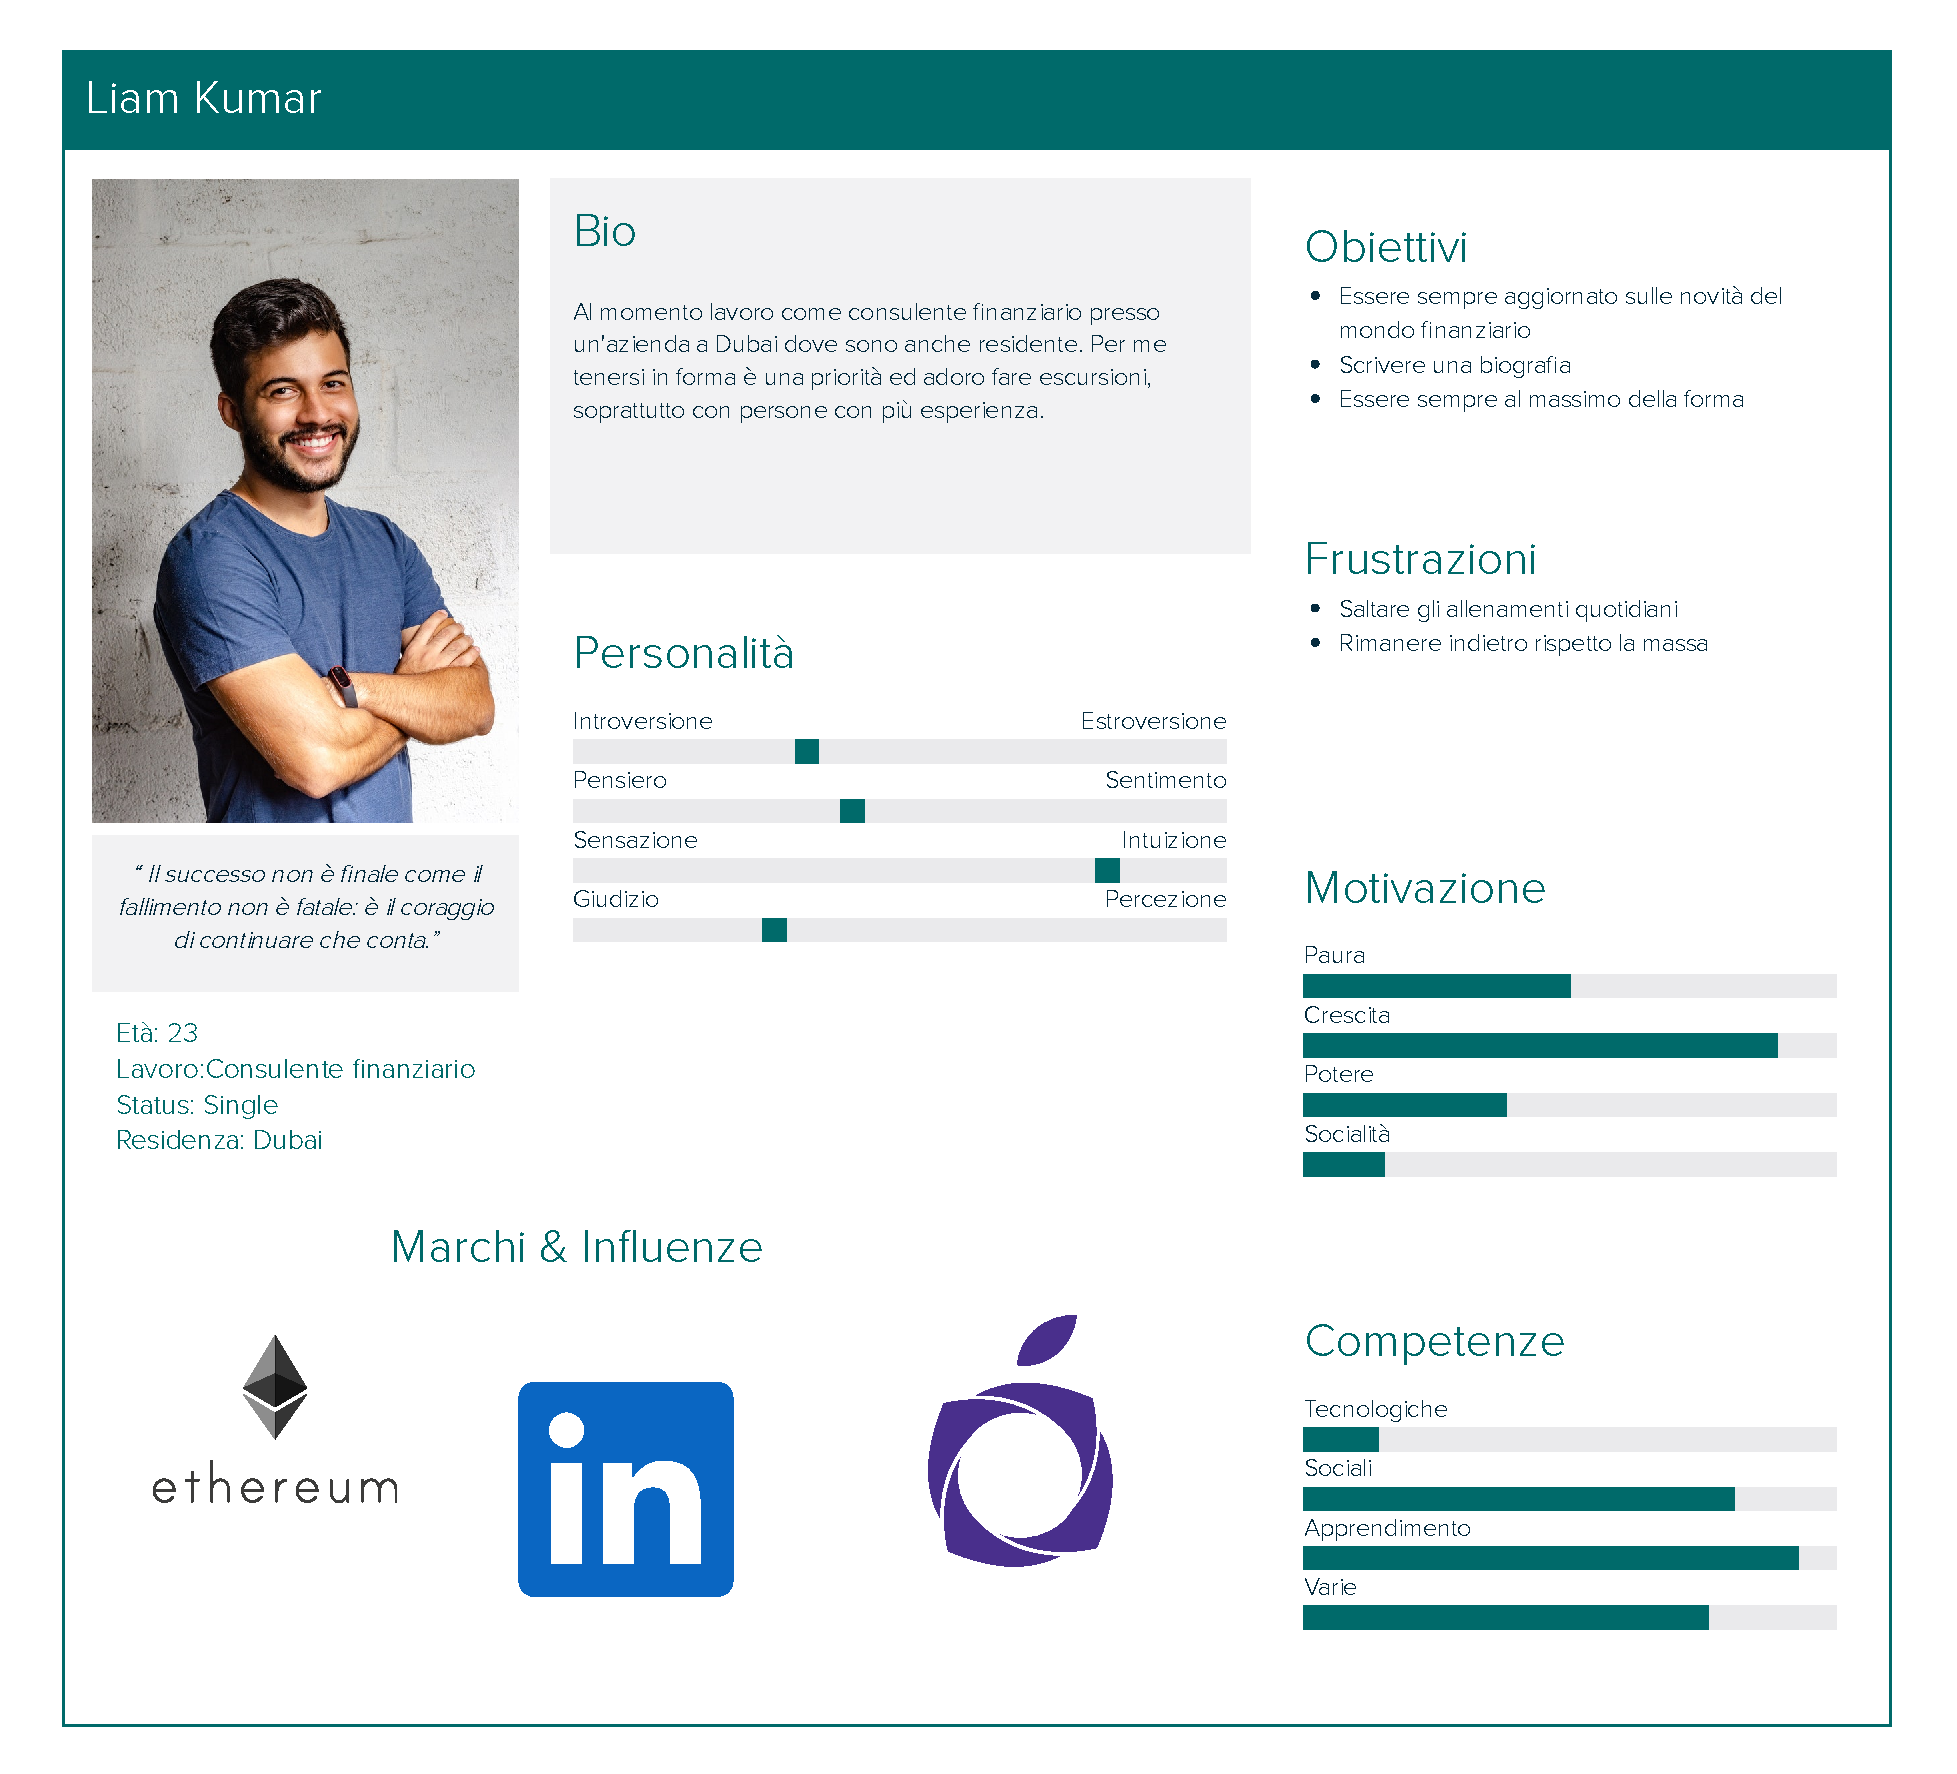
\includegraphics[width=\textwidth]{./personas/personas-kumar.pdf}
\end{figure}

È stato scelto di differenziare le caratteristiche delle personalità prese in analisi, in modo da coprire una maggiore fetta di utenza.
\begin{figure}[!htbp]
	\centering
	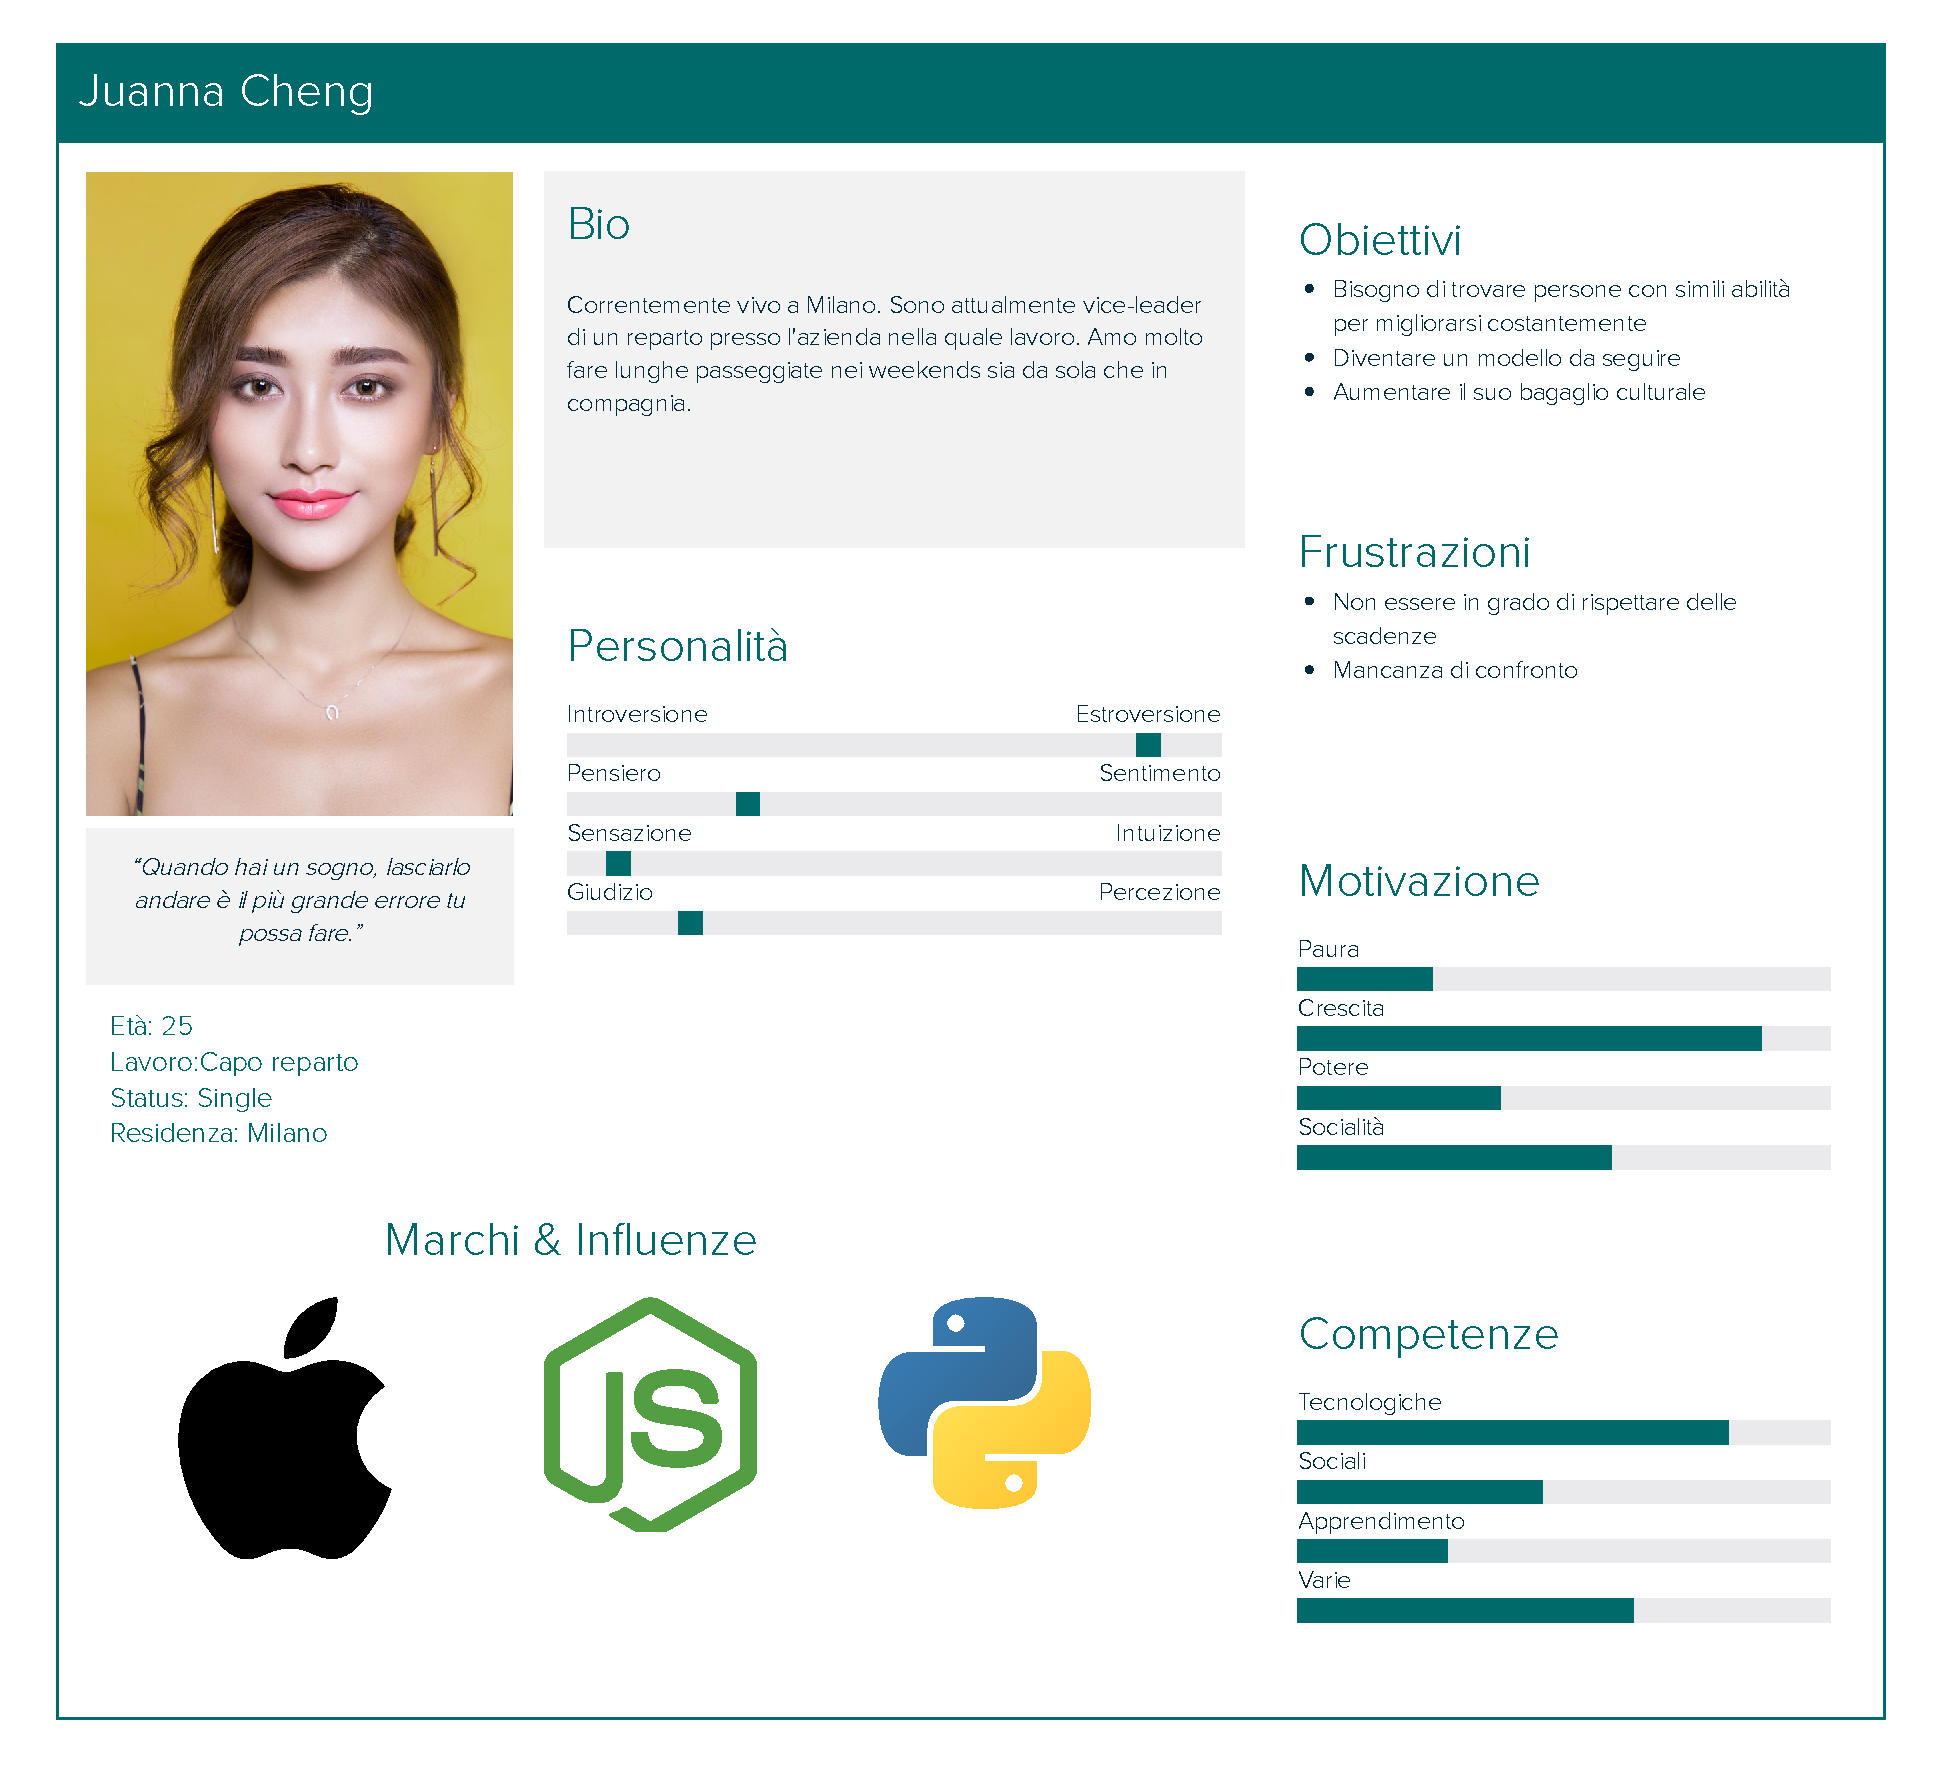
\includegraphics[width=\textwidth]{./personas/personas-cheng.pdf}
\end{figure}

\newpage
Modellando dei potenziali utenti è possibile comprendere quelli che potrebbero essere i punti critici del prodotto.
\begin{figure}[!htbp]
	\centering
	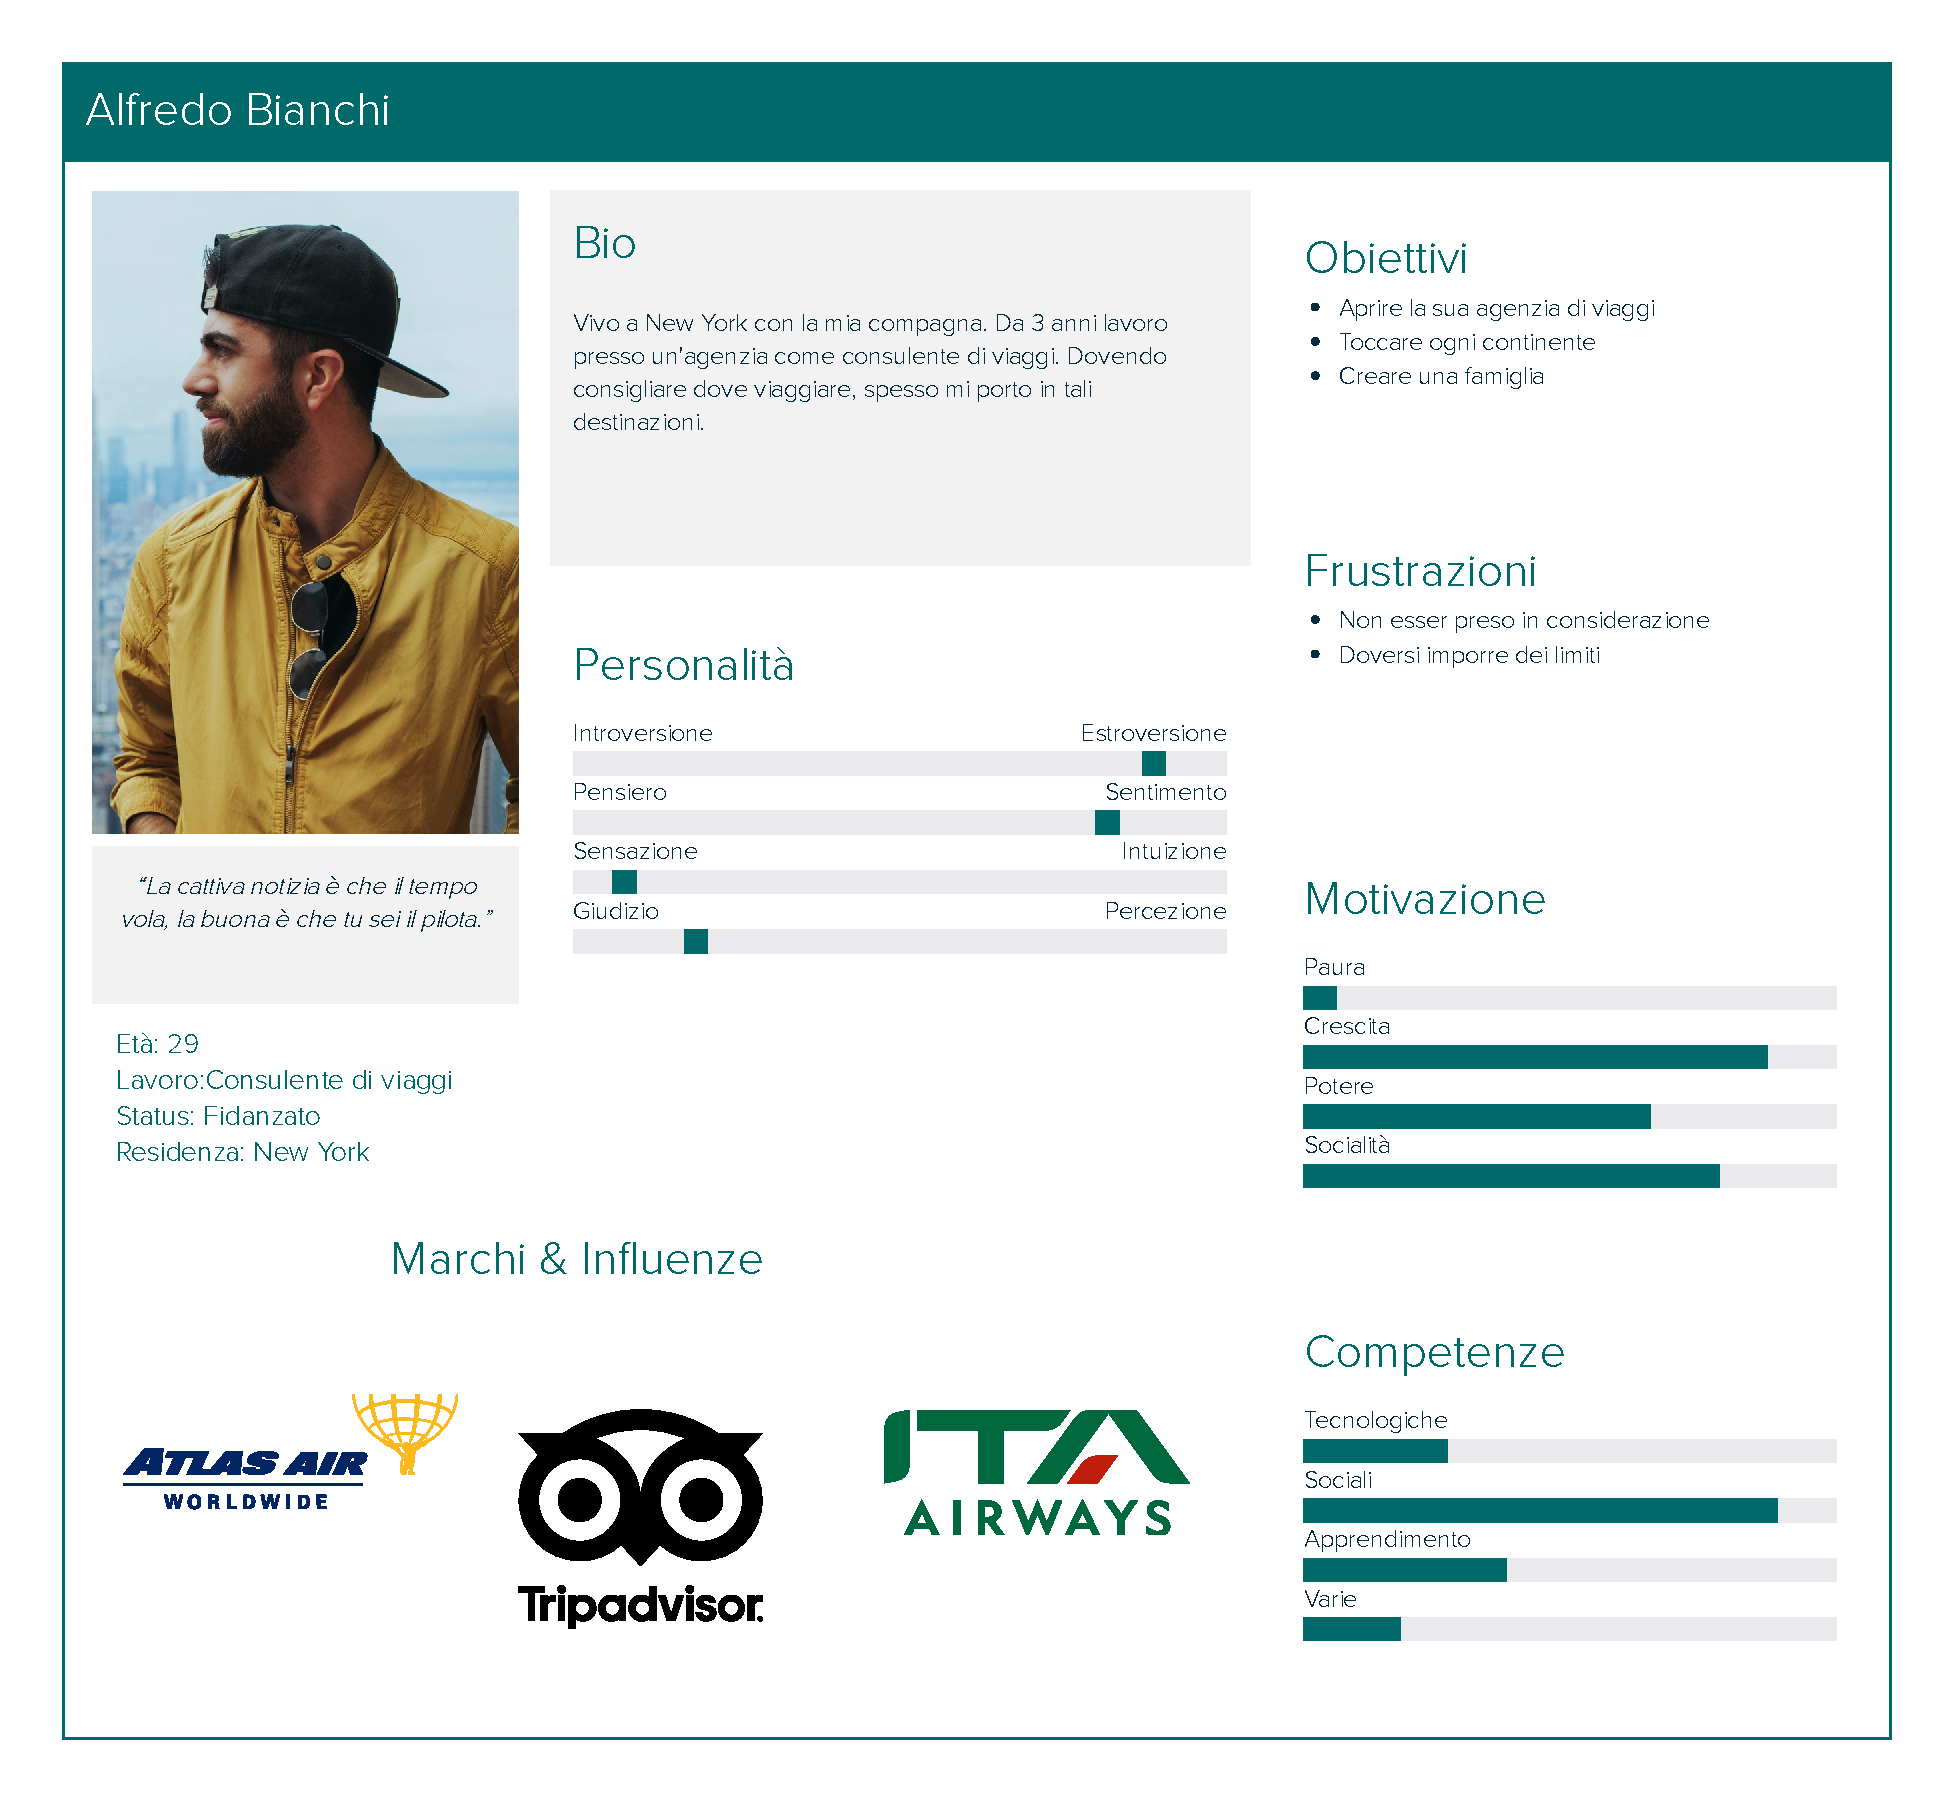
\includegraphics[width=\textwidth]{./personas/personas-bianchi.pdf}
\end{figure}

Come si può notare dai precedenti modelli, non ci si è concentrati soltanto su probabili \textit{skills} degli utenti, ma anche sul loro
temperamento: si ritiene fondamentale, infatti, adattare l'esperienza utente in modo che possa risultare piacevole a tutte le diverse personalità.

\newpage
\subsubsection{Prototipazione dell'esperienza utente}
Attraverso una fase di \textbf{brainstorming} sono state generate idee per sfruttare le opportunità e risolvere i problemi emersi durante la creazione delle \textit{personas}.
La raccolta di opinioni e suggerimenti dei componenti del team di progettazione ha analizzato anche le proposte più semplici ed intuitive: è stato ritenuto importante, infatti, valutare ogni
possibilità nata dal processo creativo. \\
Una volta approfondite le proposte, è stato deciso di realizzare dei prototipi dinamici con un tool di \Gls{CASE}; nello specifico, la scelta di quest'ultimo è ricaduta su \textit{Figma}.\\

Periodicamente ogni prototipo è stato discusso e rielaborato, in un processo coinvolgente tutti i membri del team e avente come oggetto, in particolare, le seguenti analisi:
\begin{itemize}
	\item Facilità di navigazione;
	\item Tempo di reperimento dei contenuti;
	\item Coerenza nella creazione di nuovi contenuti.
\end{itemize}

Progettare l'interazione tra utenti e prodotto è un processo complicato e spesso anche dispendioso. \\
Una possibile soluzione a questo problema, però, esiste: si tratta di un metodo molto utilizzato in
\textbf{UX Design}, avente lo scopo di ridurre al minimo i test utente. Tale processo è noto come \textit{valutazione euristica}. \\

Le \textbf{Euristiche di Nielsen} sono il cardine dell'esperienza utente ideata. \\
Il focus dell'analisi è stato rivolto verso lo \textit{stato del sistema}, con particolare attenzione agli stati di \textit{caricamento} e di \textit{errore};
si è ritenuto opportuno, in queste condizioni, fornire all'utente dei feedback. \\
Per quanto riguarda le situazioni di errore è stata adottata una politica di \textit{problem avoidance} piuttosto che di \textit{problem solving}: ciò non implica,
ovviamente, che le circostanze di errore non siano state gestite o degnate della giusta attenzione. Si è preferito, però, concentrarsi sul \textit{prevenire} gli errori.
Ove possibile, infatti, sono stati posti dei "limiti": grazie alla loro presenza, non sarebbe possibile procedere con l'utilizzo di una particolare funzionalità se
i requisiti necessari per un corretto funzionamento di quest'ultima non fossero rispettati. \\
Le funzionalità più "comuni", in quanto di prassi nel mondo del social networking, si trovano sotto nomi ben noti: una delle motivazioni di questa scelta è stata sicuramente la volontà di
creare una corrispondenza tra il sistema e il mondo reale. La motivazione principale, però, è stata la volontà di ottenere una sorta di \textit{continuità} nell'utilizzo del prodotto: sfruttando convenzioni ormai
consolidate nell'esperienza utente, è stato ritenuto naturale e improntato a una migliore comprensione del funzionamento dell'applicativo sfruttare i meccanismi
e comportamenti - che per un utente abituale risultano involontari - che entrano in gioco nell'utilizzo di un'applicativo informatico. \\
L'interfaccia non presenta limitazioni; l'utente non viene mai posto in condizione di dover visualizzare funzionalità o componenti indesiderate.
È stato ritenuto però necessario stabilire delle eccezioni, relative esclusivamente ad operazioni \textit{distruttive}, che potrebbero causare modifiche permanenti ed irreversibili
ai contenuti inseriti. Tali operazioni presentano dunque la necessità di essere confermate prima di essere portate a termine: risulta chiara, anche qui, la volontà di evitare
situazioni di disagio causate da meri errori dell'utente.\\
L'interfaccia realizzata per il software risulta essere estremamente minimalista; i contenuti più importanti sono posti in risalto attraverso sfumature, colori, elevazione ed un
posizionamento strategico delle informazioni. \\
Le scelte di design sono dunque improntate a creare un ambiente visivo semplice e di immediata comprensione.
Ci si trova in presenza di un ambiente totalmente isolato, in cui le diverse schermate sono caratterizzate da una forte
\textbf{consistenza}. Per \textit{consistenza} si intende il mantenimento di una linea generale di presentazione di contenuti attraverso
l'intero applicativo: le diverse interfacce non presentano mai cambi di layout estremi, garantendo una maggiore velocità d'apprendimento agli utenti. \\

Prima di raffinare l'esperienza utente è stato ritenuto necessario coinvolgere un ristretto bacino d'utenza per ottenere riscontri esterni
rispetto al contesto di prototipazione e sviluppo.

\newpage
\subsubsection{Definizione di uno stile di design}
Per raffinare l'esperienza utente è stato ritenuto un buon approccio quello di affidarsi ad uno specifico \Gls{UI Design System}.
La scelta è stata effettuata tra diversi sistemi concorrenti, ricadendo infine su
\textbf{Material}\footnote{Material è un design system creato da Google per facilitare lo sviluppo di UX di altissima qualità per Android, iOS, Flutter, e Web-App.}.

\FloatBarrier
\begin{figure}[htbp!]
	\centering
	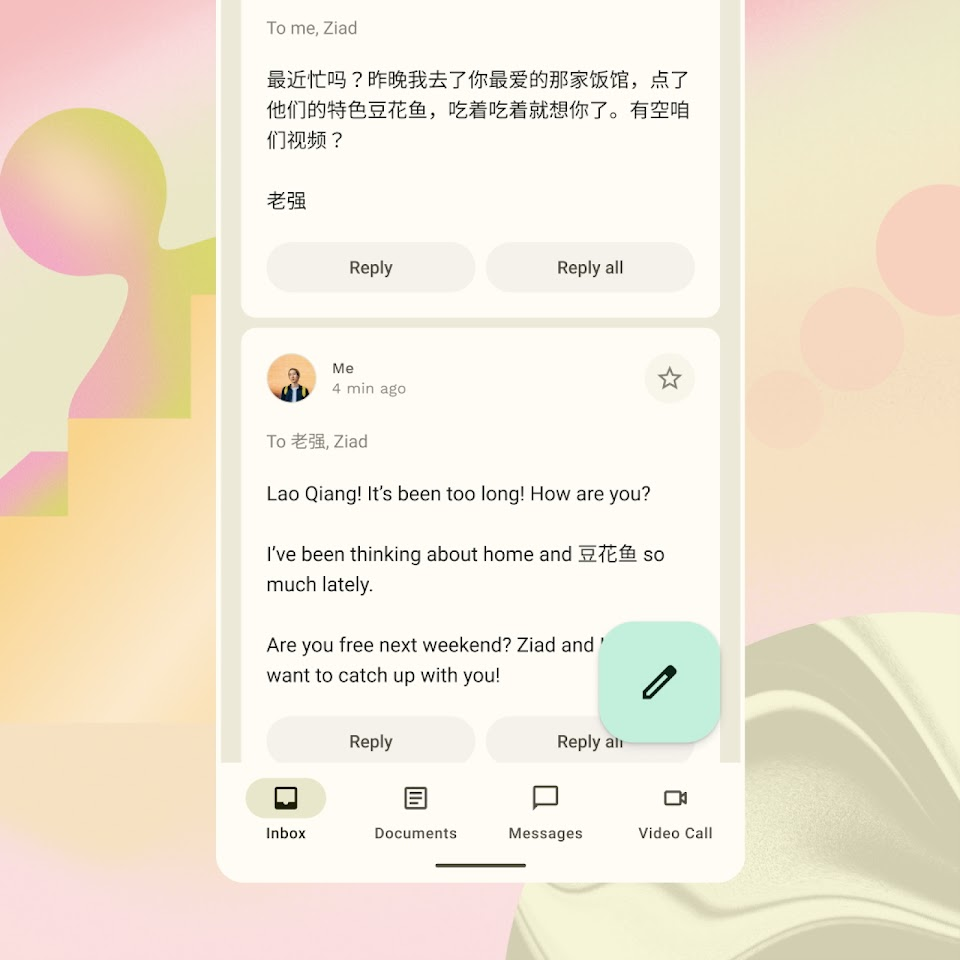
\includegraphics[height=7cm]{usability/material3.jpg}
\end{figure}
\FloatBarrier

Material Design si ispira al mondo fisico, includendo riflessi e ombre. Tipografie, griglie, spazi e colori creano gerarchie finalizzate a rendere l'utilizzatore totalmente immerso.
Gli effetti di movimento mirano a focalizzare l'attenzione generando continuità spaziale attraverso feedback e transizioni.
Le componenti sono altamente dinamiche, si trasformano e organizzano l'ambiente in base alle interazioni, generando altre trasformazioni.\\
Le componenti Material sono blocchi interattivi che formano l'interfaccia utente.
Queste includono stati built-in system per comunicare focus, selezione, attivazione, errore, hovering, pressione, trascinamento, e disabilitazione. \\\\
Ogni componente è realizzata avendo specifiche caratteristiche e finalità, tra le quali:
\begin{itemize}
	\item \textbf{Esposizione} - Piazzare ed organizzare contenuti correlati usando componenti come \textit{card} e \textit{liste};
	\item \textbf{Navigazione} - Consentire agli utenti di muoversi nel prodotto finito utilizzando \textit{drawer} o \textit{tabs};
	\item \textbf{Azioni} - Consentire agli utenti di eseguire task utilizzando componenti di alto rilievo, come i \textit{floating action button};
	\item \textbf{Input} - Consentire agli utenti di inserire informazioni o selezionare tra un certo numero di opzioni, attraverso \textit{campi di testo dinamici} e \textit{chips};
	\item \textbf{Comunicazione} - Dare informazioni agli utenti attraverso \textit{snackbar}, \textit{toast} e \textit{dialog}.
\end{itemize}

\newpage
\subsection{Mock-Up dell'applicazione}
Vengono ora mostrati i Mock-Up dei casi d'uso significativi dettagliati nella sottosezione precedente.
\subsubsection{Inserimento itinerario}
Il processo di inserimento di un itinerario consiste in tre fasi:
\begin{itemize}
	\item Inserimento informazioni sull'itinerario;
	\item Inserimento mappa itinerario;
	\item Inserimento foto itinerario.
\end{itemize}

Sono presentati i Mock-Up che rappresentano un inserimento fittizio, con scopo illustrativo.

\begin{figure}[htbp]
	\centering
	\begin{minipage}[t]{0.4\textwidth}
		\resizebox{\textwidth}{!}{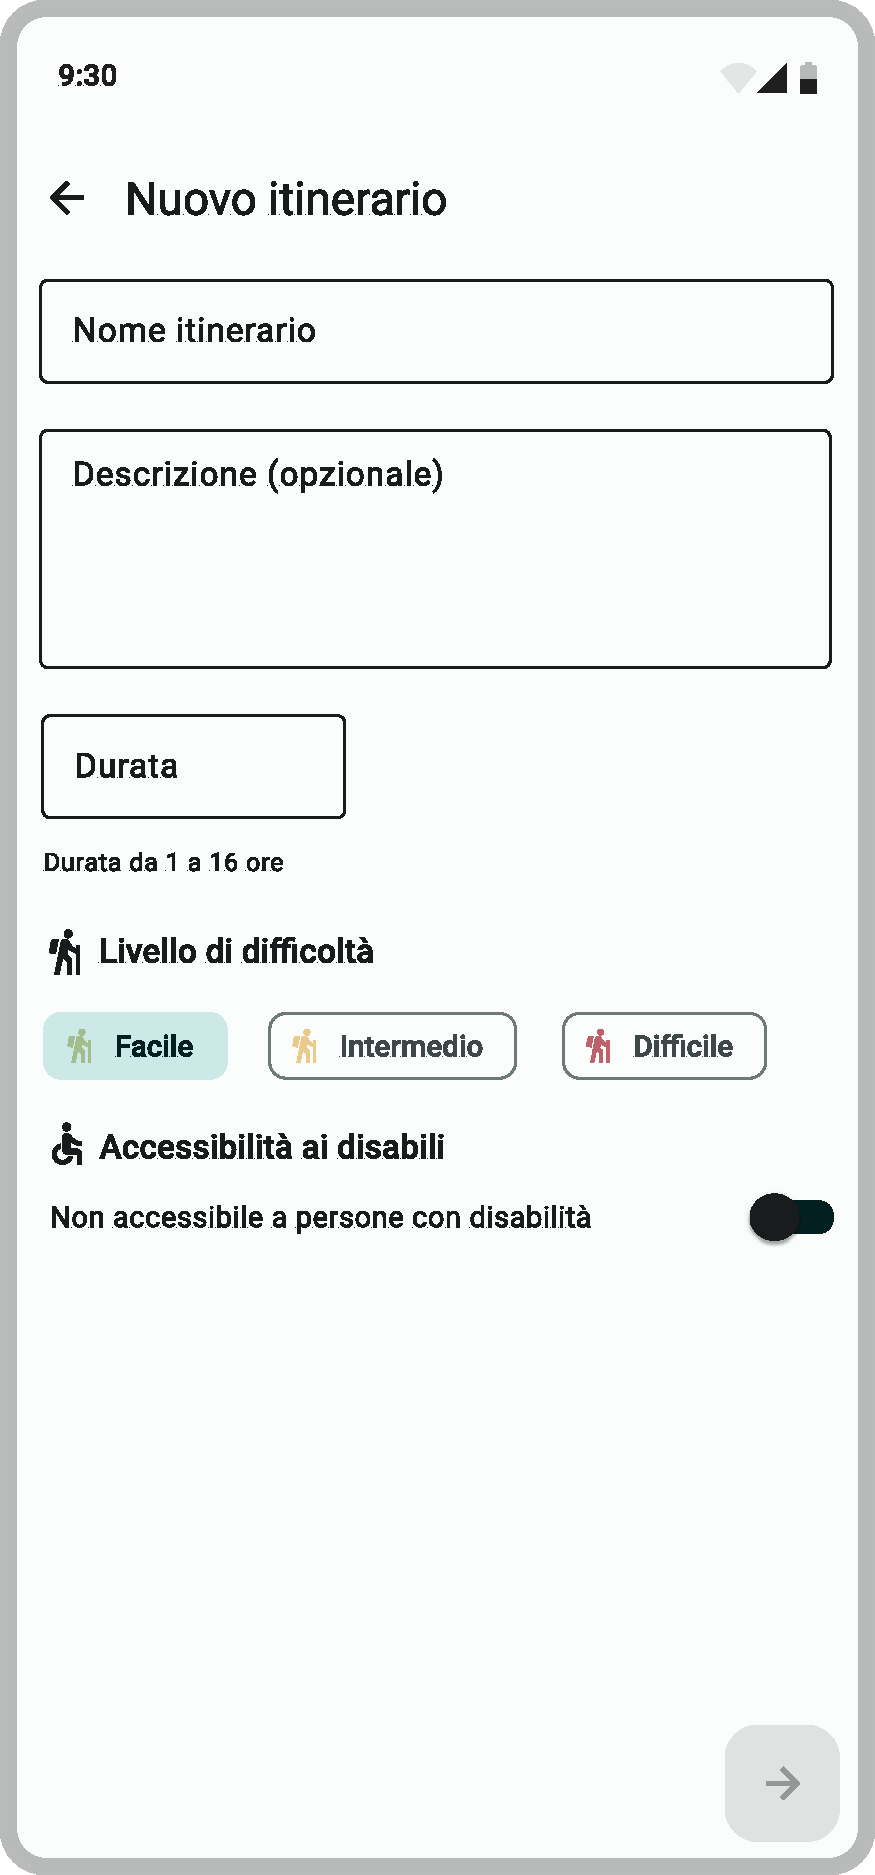
\includegraphics{./mockup/CreateRouteInfoUi-empty.pdf}}
		\caption{Inserimento informazioni - form vuoto}
	\end{minipage}
	\hfill
	\begin{minipage}[t]{0.4\textwidth}
		\resizebox{\textwidth}{!}{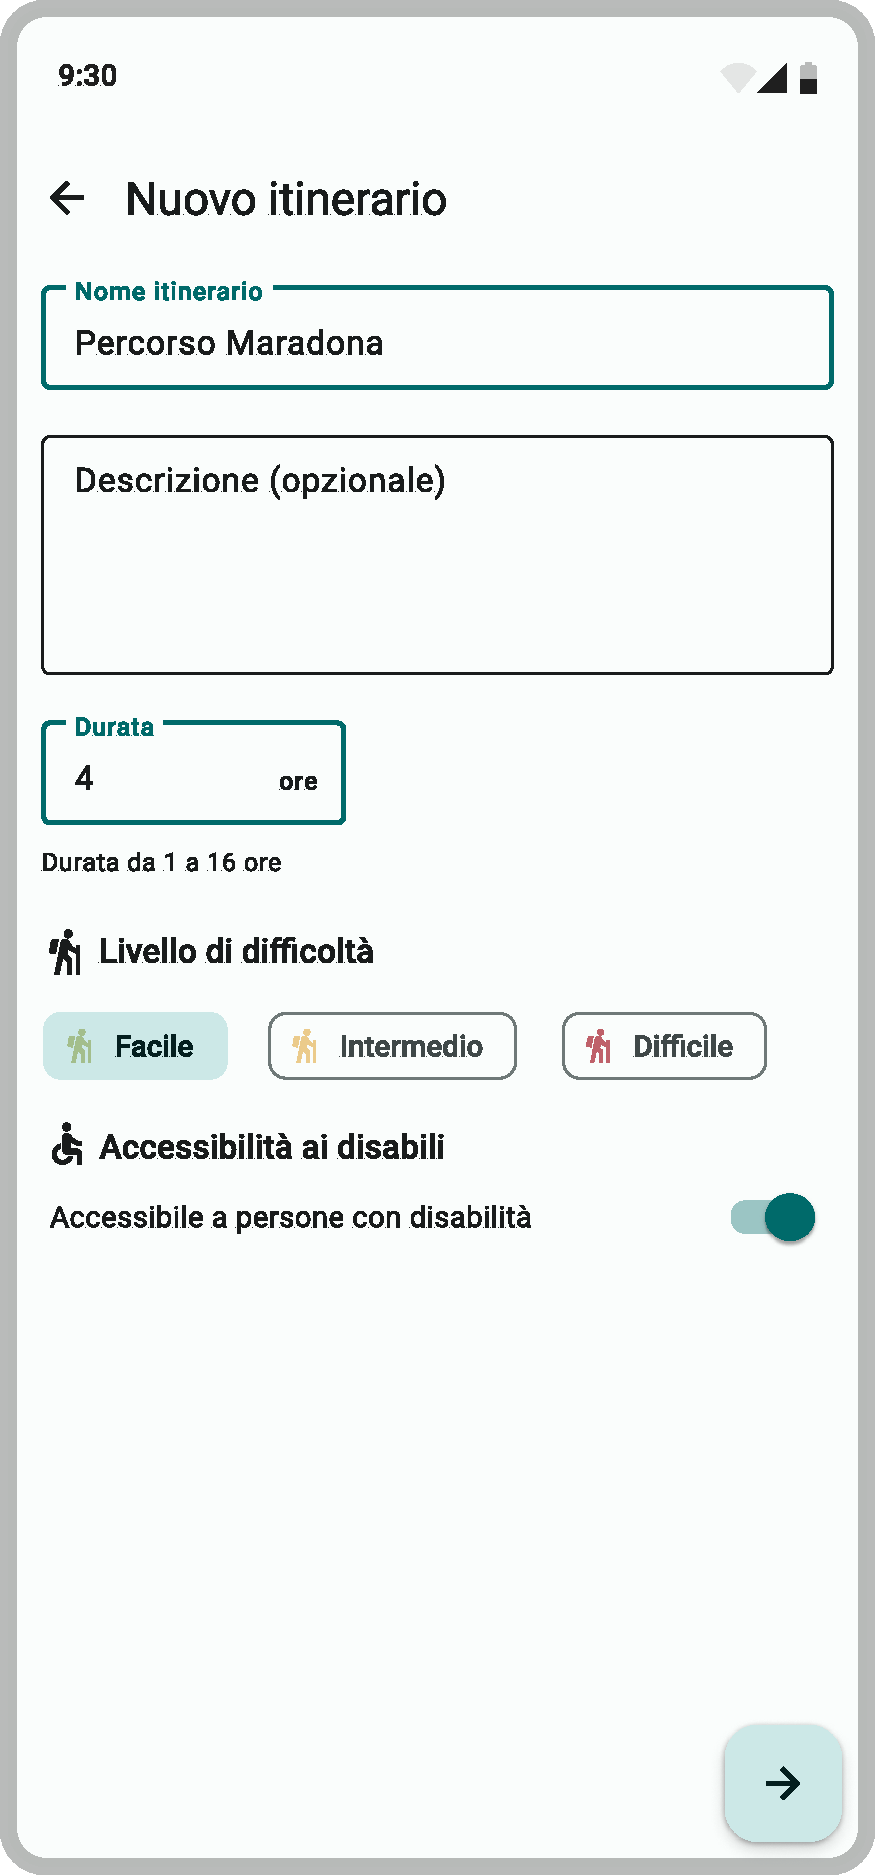
\includegraphics{./mockup/CreateRouteInfoUi.pdf}}
		\caption{Inserimento informazioni - compilato}
	\end{minipage}
\end{figure}

\newpage
Il processo di inserimento della mappa può avvenire sia interagendo con la mappa interattiva sia importando
un file GPX dall'apposito menu. In entrambi i casi è possibile ricercare una posizione per visualizzarla sulla mappa
ed eventualmente apporre i marker; inoltre è possibile eliminare i marker inseriti.

\begin{figure}[htbp]
	\centering
	\begin{minipage}[t]{0.4\textwidth}
		\resizebox{\textwidth}{!}{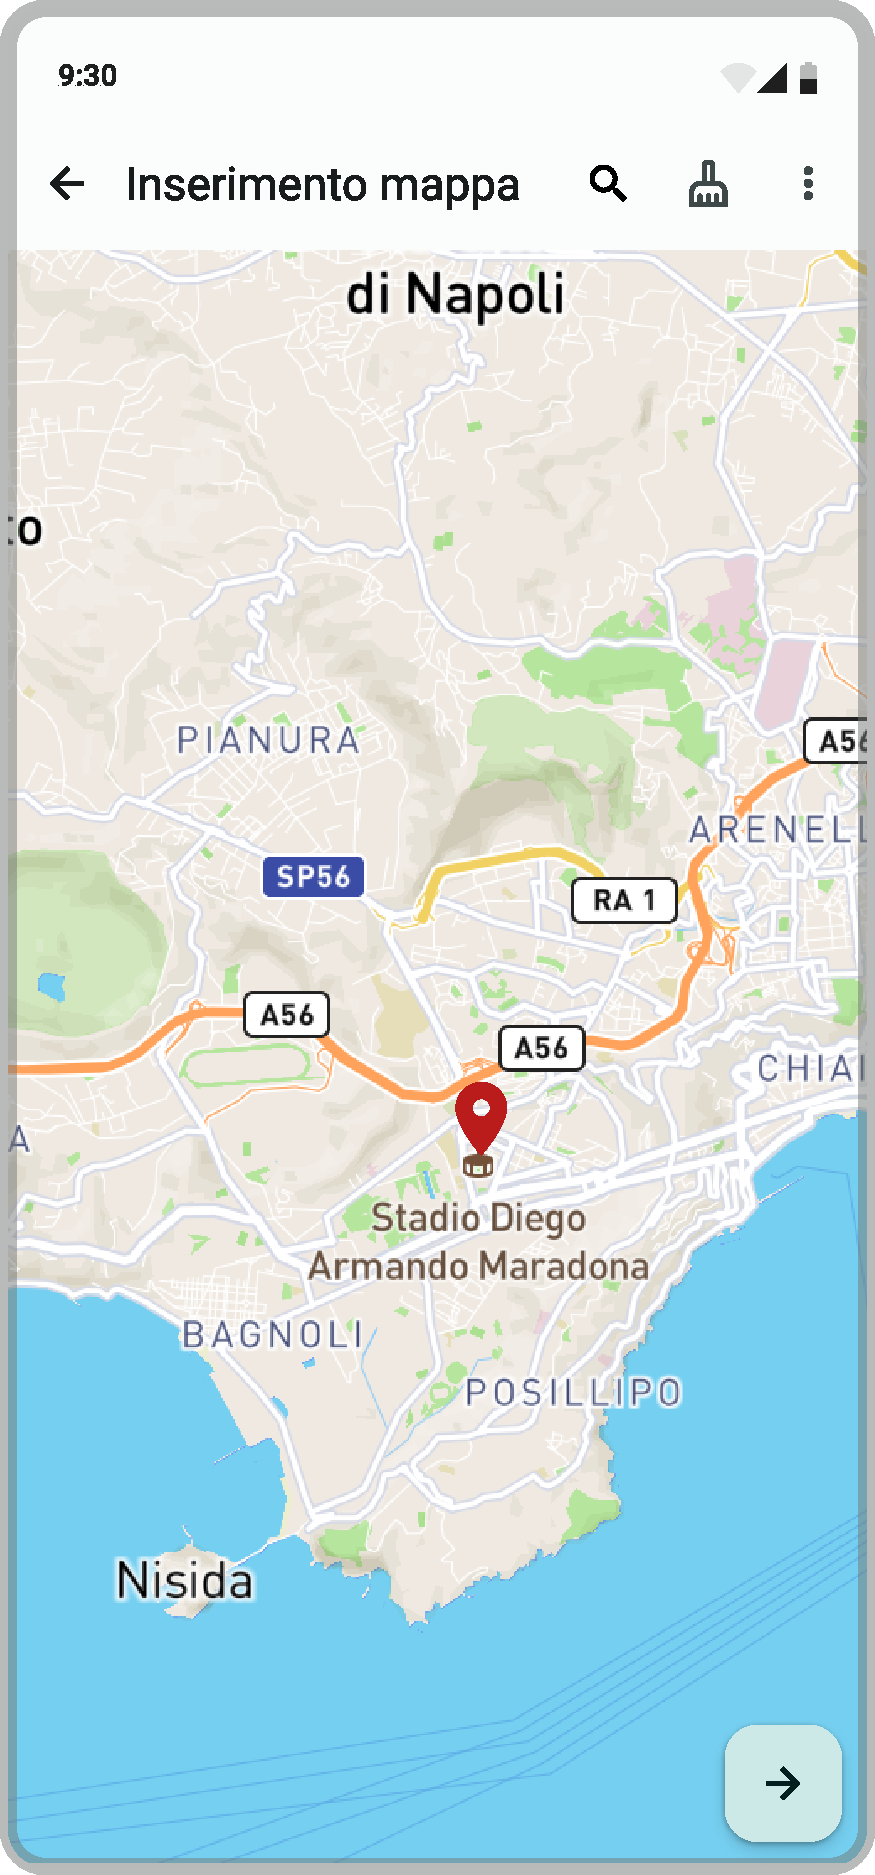
\includegraphics{./mockup/CreateRouteMapUi.pdf}}
		\caption{Inserimento mappa}
	\end{minipage}
	\hfill
	\begin{minipage}[t]{0.4\textwidth}
		\resizebox{\textwidth}{!}{\includegraphics{./mockup/CreateRouteMapUI-menu.pdf}}
		\caption{Inserimento mappa - menu}
	\end{minipage}
\end{figure}

\newpage
L'inserimento delle foto per l'itinerario usufruisce di un photo picker esterno, il quale rimanda ad una schermata di sistema
che consente la selezione di più foto, fino a un massimo di 5. Una volta effettuata la selezione desiderata, le foto appariranno
nella schermata precedente con la possibilità di eliminarle.
\begin{figure}[htbp]
	\centering
	\begin{minipage}[t]{0.4\textwidth}
		\resizebox{\textwidth}{!}{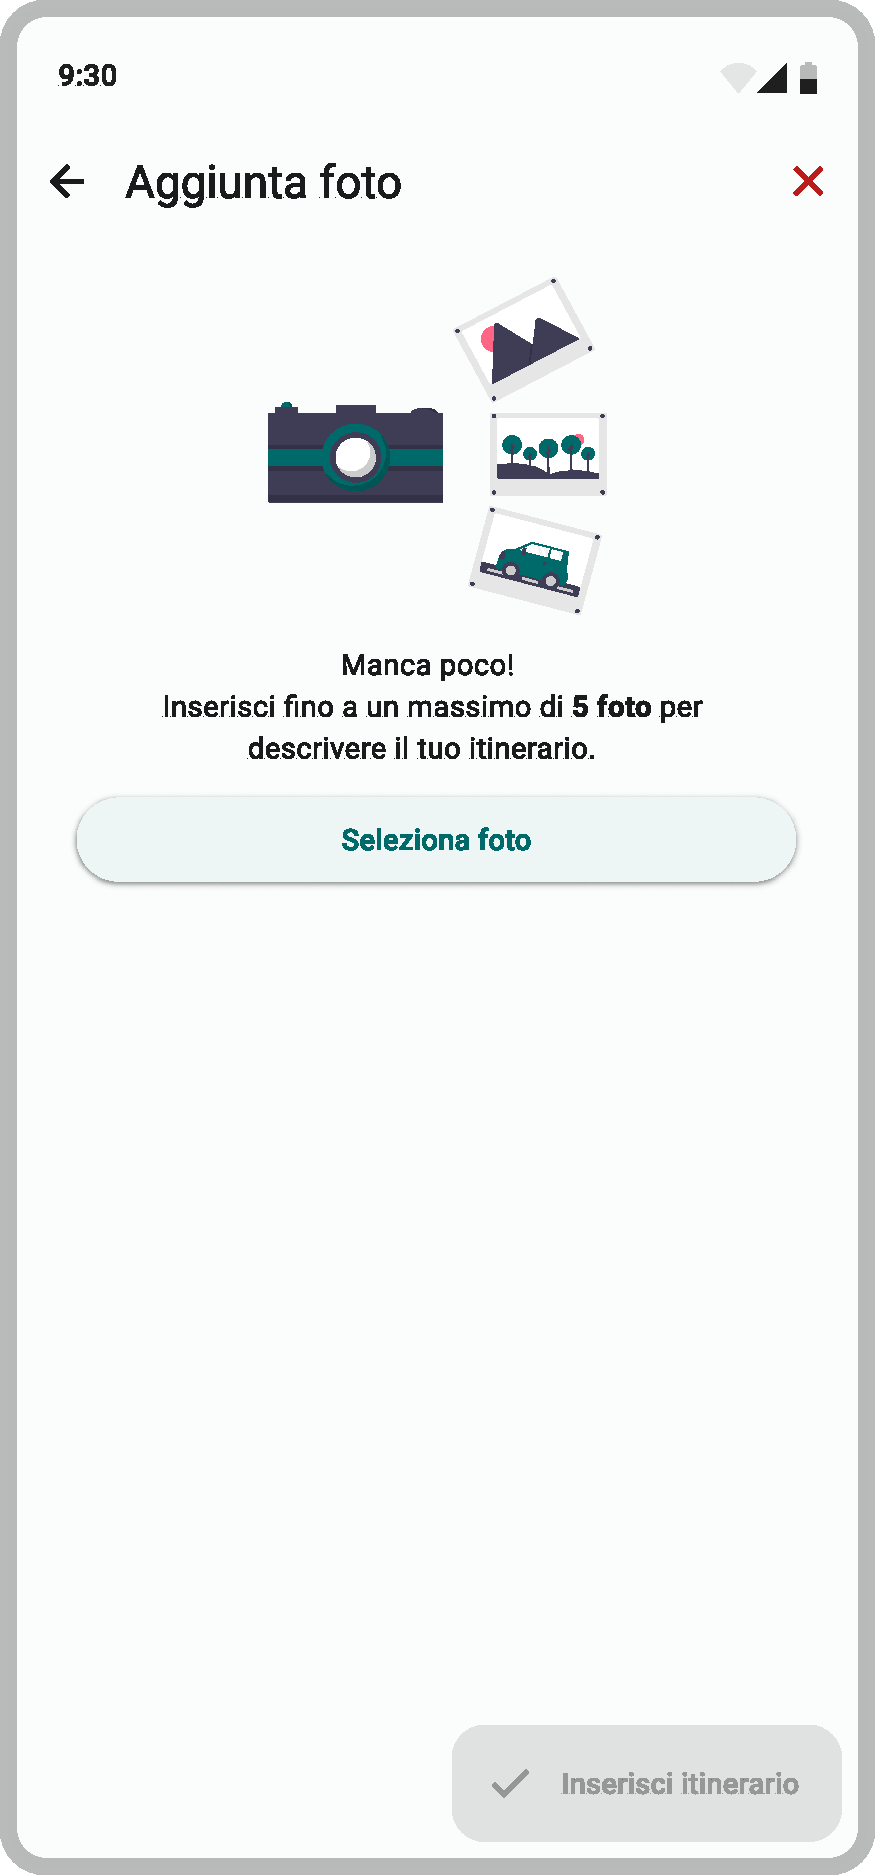
\includegraphics{./mockup/CreateRoutePhotosUi.pdf}}
		\caption{Inserimento foto}
	\end{minipage}
	\hfill
	\begin{minipage}[t]{0.4\textwidth}
		\resizebox{\textwidth}{!}{\includegraphics{./mockup/CreateRoutePhotosUi_withphotos.pdf}}
		\caption{Inserimento foto - foto inserite}
	\end{minipage}
\end{figure}

È importante sottolineare che - per ridurre al minimo i possibili errori nell'inserimento - le \textit{affordance}
che consentono la navigazione tra le diverse fasi dell'inserimento restano disattivate fino all'inserimento di input adeguati.\\

Una caratteristica di particolare rilevanza è il \textit{salvataggio dello stato} dell'inserimento tra le schermate: sarà quindi
possibile navigare tra di esse senza perdere i dati inseriti. \\

\newpage
\subsubsection{Segnalazione itinerario}
La segnalazione di un itinerario avviene tramite una full dialog, a seguito del riempimento dell'apposito form.
\begin{figure}[htbp]
	\centering
	\begin{minipage}[t]{0.4\textwidth}
		\resizebox{\textwidth}{!}{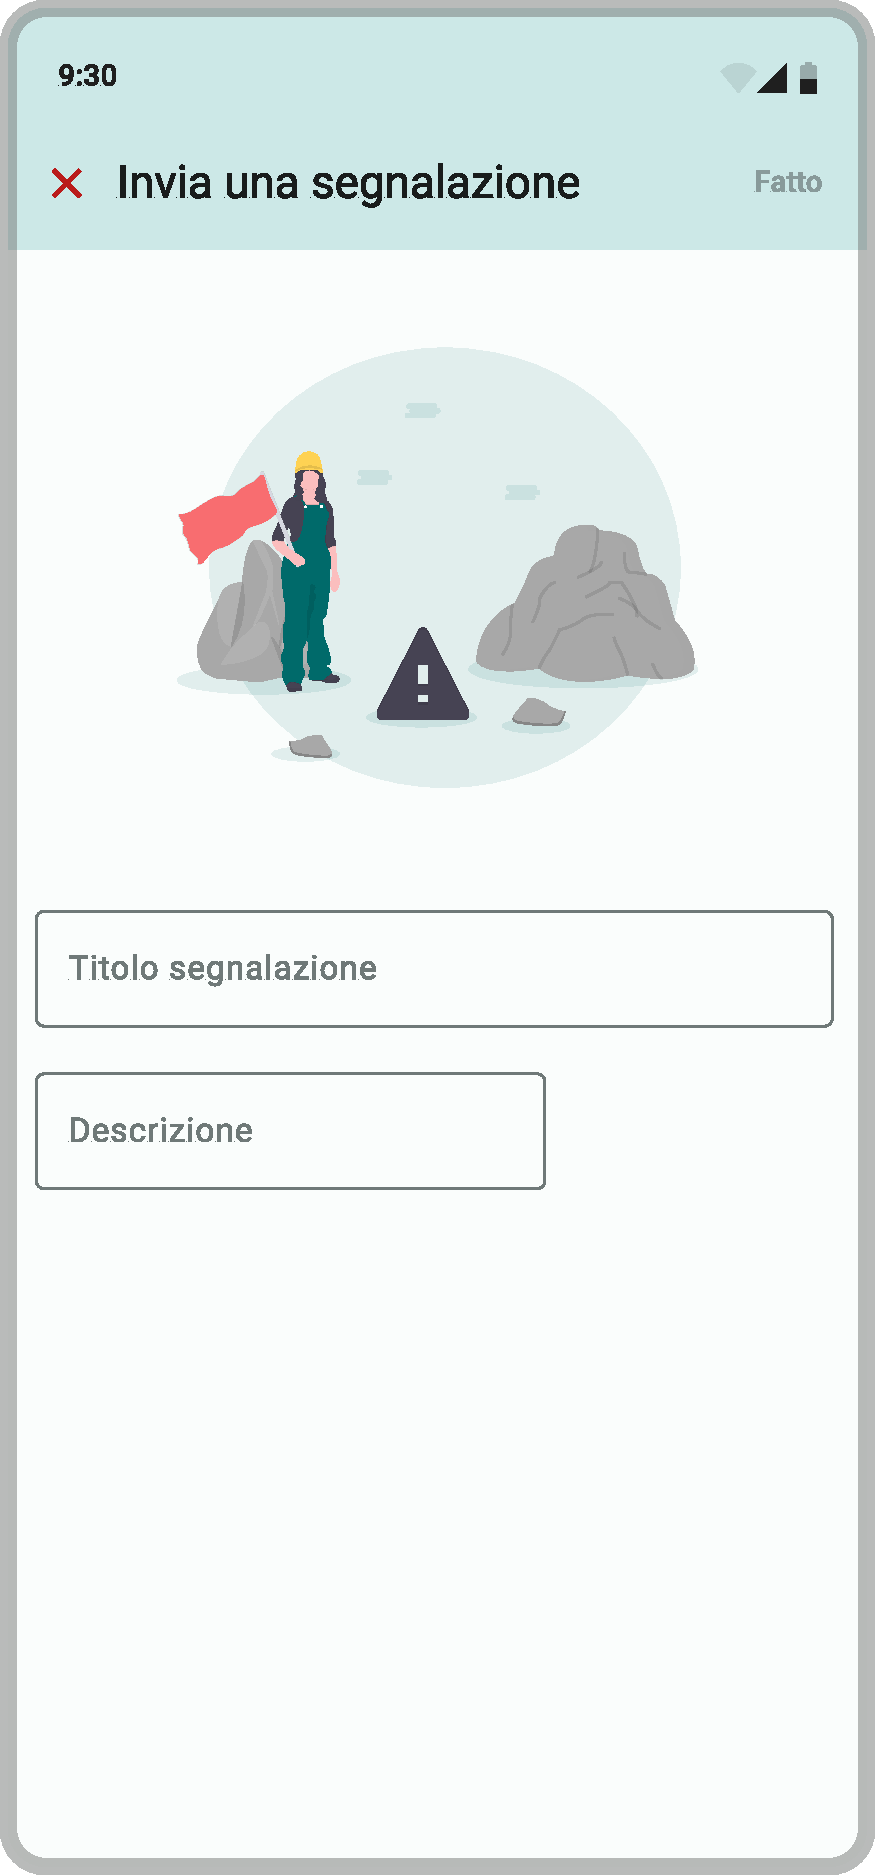
\includegraphics{./mockup/ReportRouteUi-empty.pdf}}
		\caption{Segnalazione - form vuoto}
	\end{minipage}
	\hfill
	\begin{minipage}[t]{0.4\textwidth}
		\resizebox{\textwidth}{!}{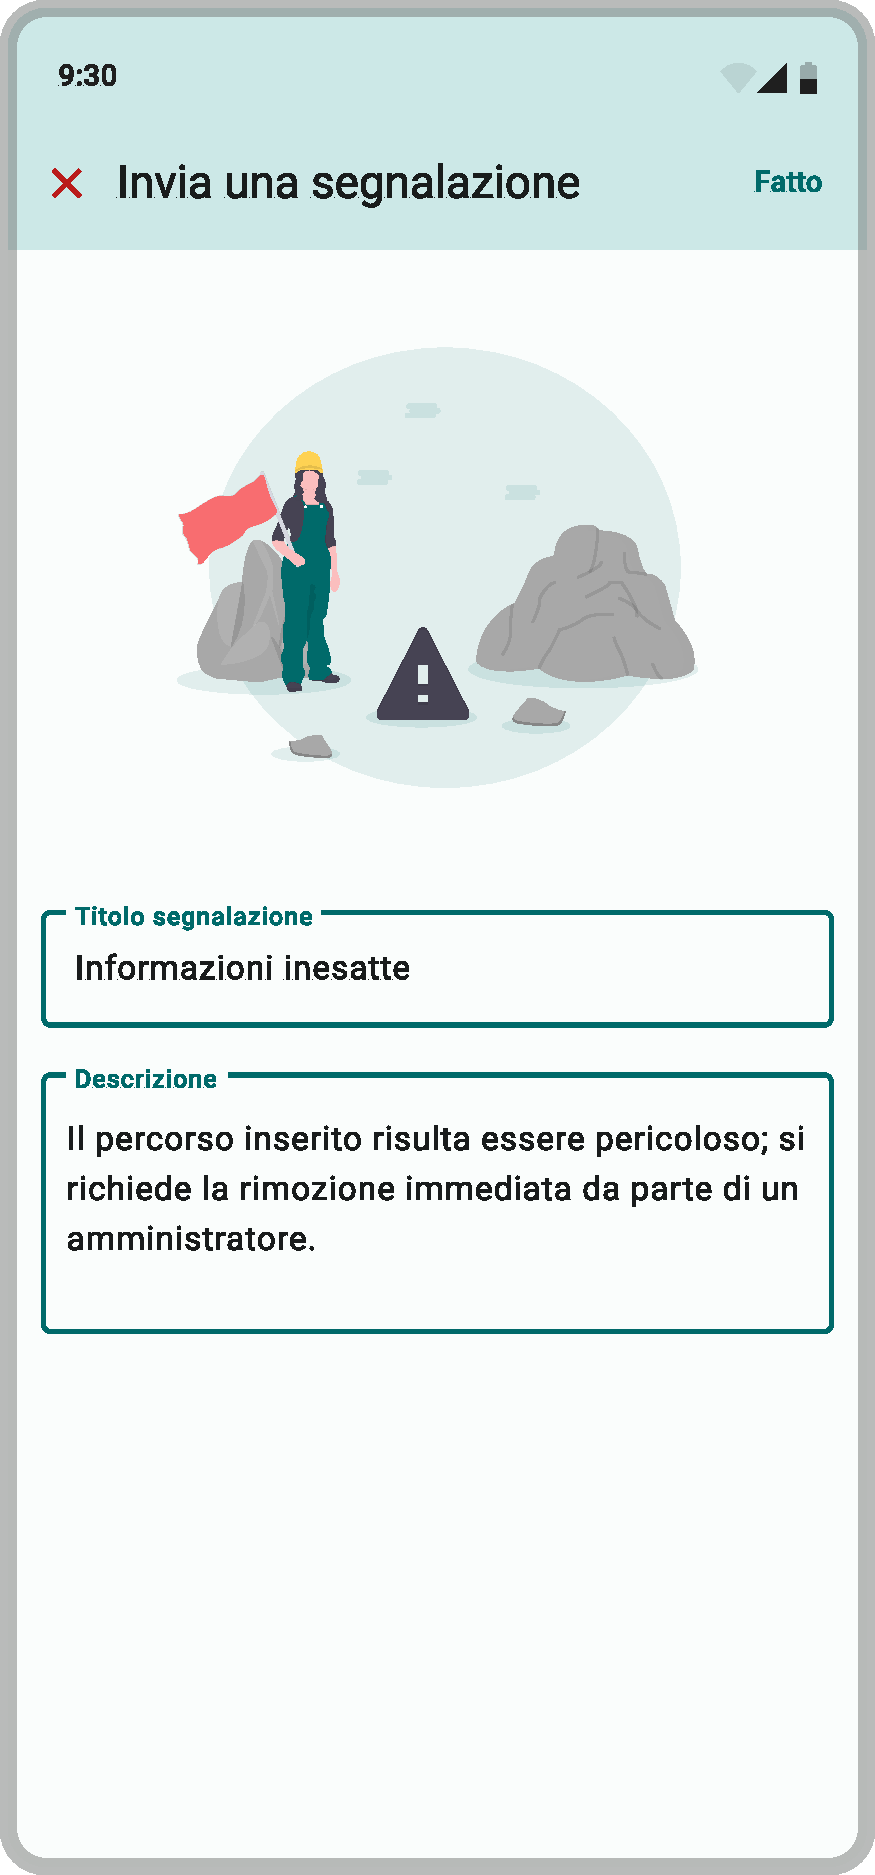
\includegraphics{./mockup/ReportRouteUi.pdf}}
		\caption{Segnalazione - compilato}
	\end{minipage}
\end{figure}

\newpage

\subsection{Valutazione dell'usabilità a priori}
Una parte fondamentale del processo creativo alla base dello sviluppo di un'applicazione è capire la direzione da seguire per migliorare l’esperienza dei clienti.
Al fine di rendere la user experience quanto più piacevole possibile si è ricorso alla messa in pratica di alcune tecniche, con il fine di testare l’usabilità del prodotto.
L’approccio adottato richiede l'esecuzione di alcun task ad un gruppo di utenti con differenti retroscena. \\

Tali task possono avere un riscontro differente a seconda dell'utente:
\begin{itemize}
	\item L’utente è stato in grado di compiere il task tramite gli strumenti offerti dall’app;
	\item L’utente non è stato in grado di compiere il task tramite gli strumenti offerti dall’app;
	\item L'utente è stato in grado di compiere il task, ma ha trovato difficoltà oppure trova l'interfaccia poco intuitiva.
\end{itemize}

Verranno fornite solo indicazioni di base: il sistema dovrebbe essere intuitivo. In caso di una percentuale di riscontri altamente
negativa, il sistema sarà rielaborato alla luce dei feedback utente.

\subsubsection{Definizione dei task utente}
\begin{enumerate}
	\item \textbf{Creazione itinerario} \\
	      Hai deciso di aggiungere un nuovo itinerario all’interno della piattaforma: a questo scopo
	      dovrai andare nella sezione degli itinerari e cliccare sul bottone di creazione. Nelle schermate successive dovrai inserire le informazioni, la mappa e le foto del nuovo itinerario.
	\item \textbf{Aggiunta itinerario ad una compilation} \\
	      Hai trovato un itinerario interessante che hai scelto di inserire all’interno di una compilation. Seleziona l’icona di salvataggio per poi decidere in quale compilation inserirlo.
	\item \textbf{Segnalazione itinerario} \\
	      Hai trovato un itinerario con informazioni errate, così hai deciso di segnalarlo agli amministratori. Dalla schermata dell’itinerario in questione clicca sull'icona di segnalazione e
	      scegli un titolo e una descrizione per la segnalazione da inviare.
	\item \textbf{Contatto con autore itinerario} \\
	      Hai trovato un itinerario ma hai dei dubbi riguardo ad esso, così hai deciso di contattare l’utente che l’ha creato. Dalla schermata dell’itinerario clicca l'icona di messaggio privato per visualizzare la chat.
	\item  \textbf{Modifica immagine profilo} \\
	      Ti sei appena registrato all'applicazione, ma il tuo profilo è completamente spoglio: così hai deciso di modificare l’immagine del tuo profilo. Spostati nella sezione profilo e modifica la tua foto.
\end{enumerate}

\newpage

\subsubsection{Risultati ottenuti dallo svolgimento dei task}
Nella scelta degli utenti ai quali somministrare i task si è tenuto in considerazione di parametri quali:
\begin{itemize}
	\item \textbf{Competenza tecnologica} - per favorire un'analisi migliore dell'intuitività della UX si è preferito coinvolgere utenti abituati alle esperienze di social networking in entità diverse;
	\item \textbf{Età} - si è scelto di considerare diverse fasce di età, con lo scopo di andare oltre le innate capacità della generazione più giovane e dei "nativi digitali".
\end{itemize}

Sono elencati di seguito gli utenti che hanno partecipato allo svolgimento dei task, e le loro caratteristiche:
\begin{figure}[!htbp]
	\centering
	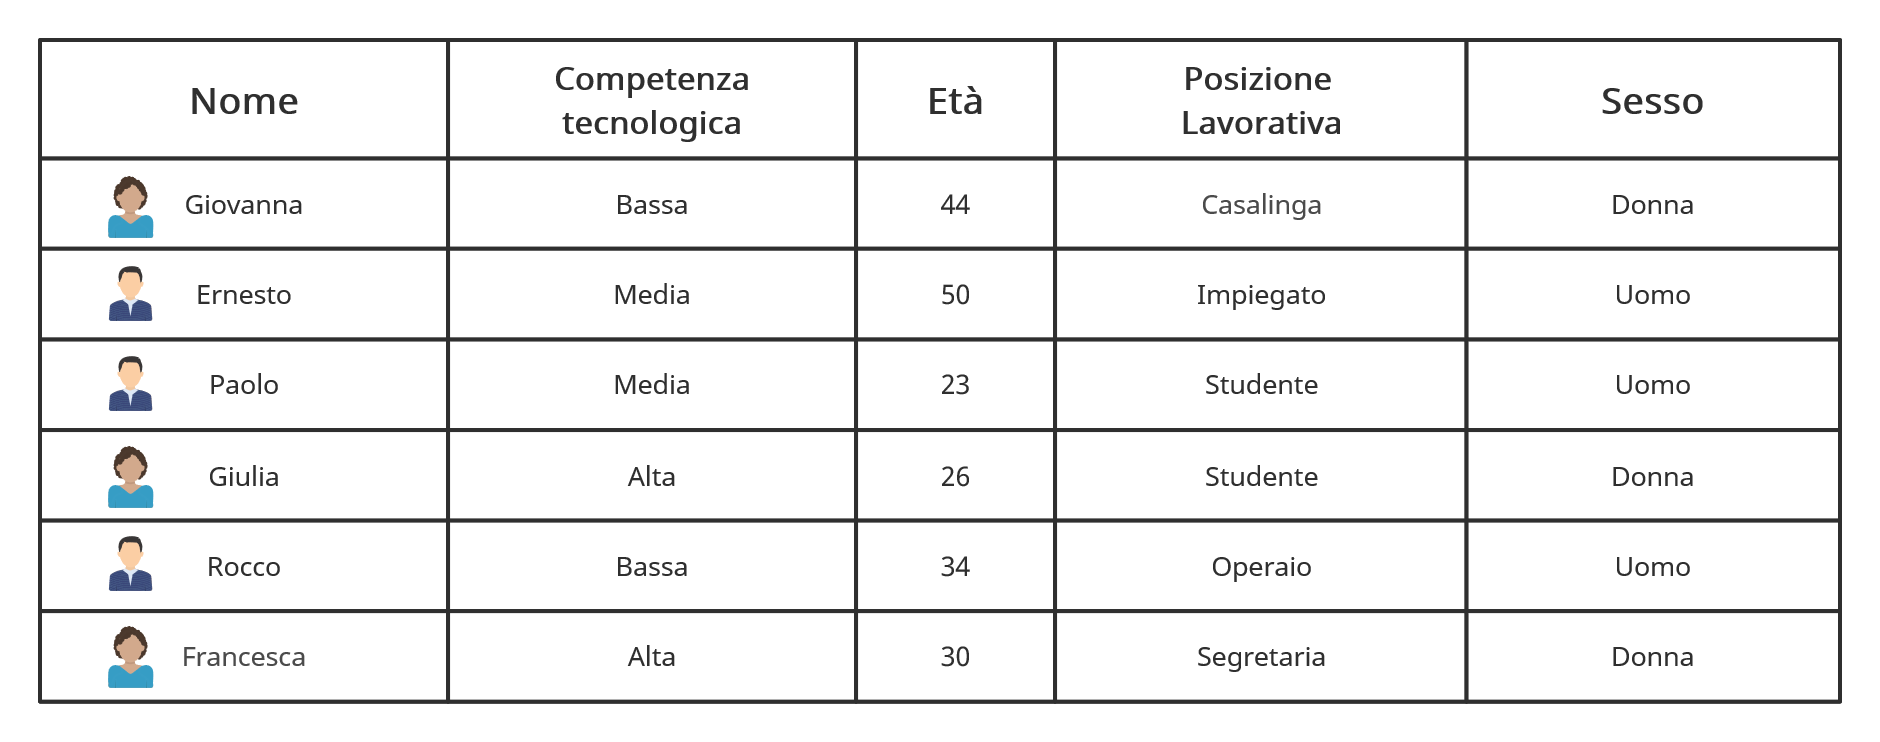
\includegraphics[width=\textwidth]{./usability/task_users.png}
	\caption{Tabella utenti scelti}
\end{figure}
\FloatBarrier

I risultati ottenuti dallo svolgimento dei task possono essere così schematizzati:
\begin{figure}[!htbp]
	\centering
	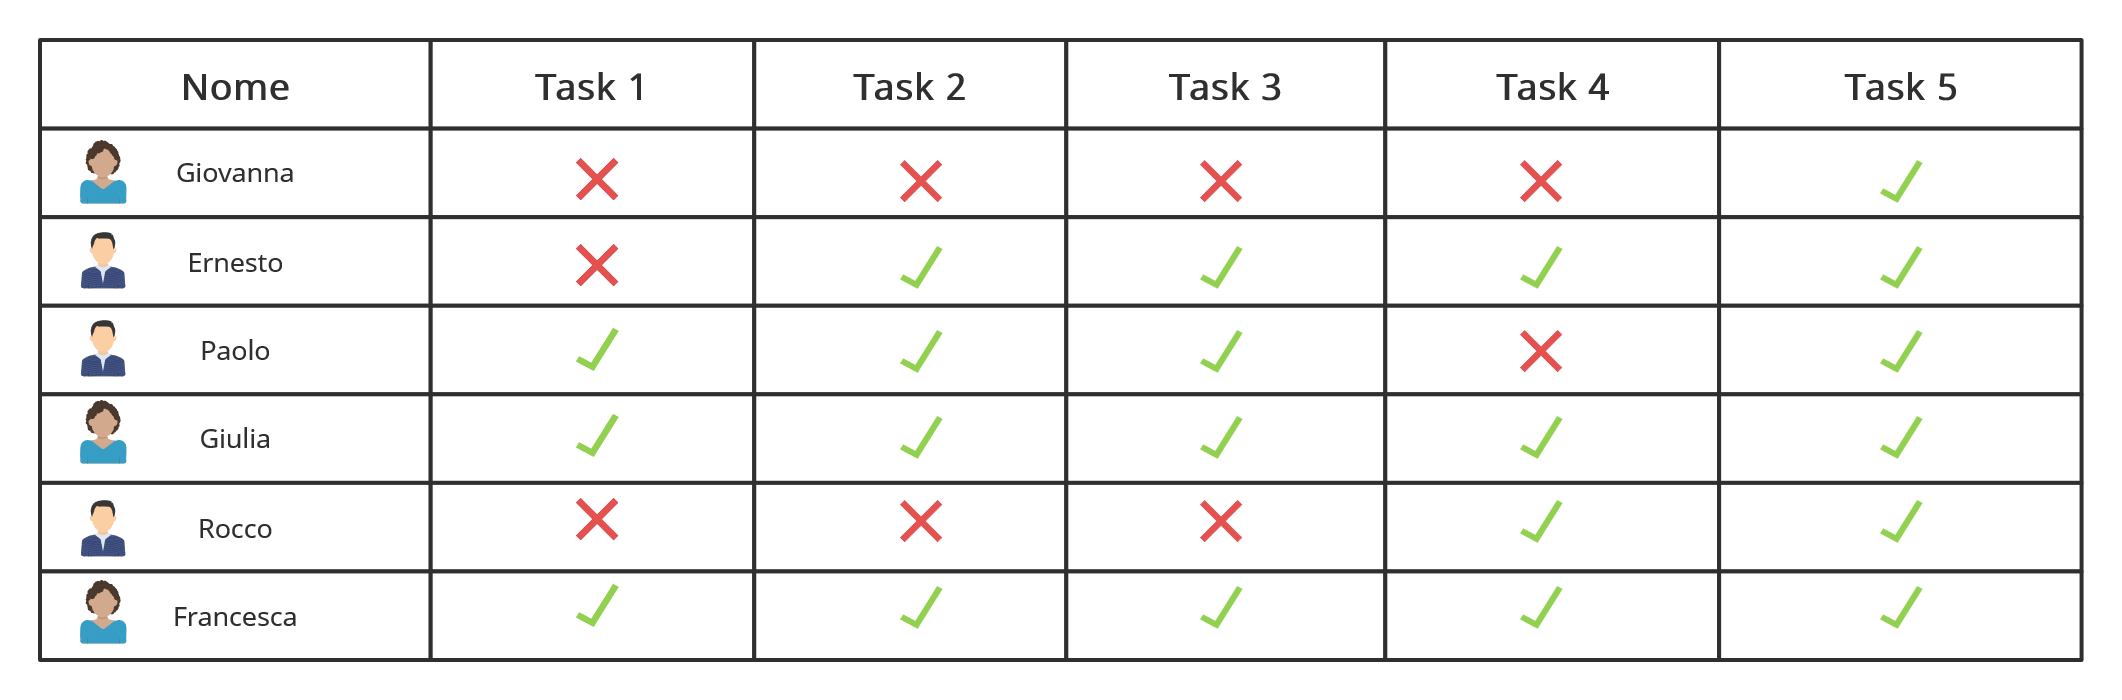
\includegraphics[width=\textwidth]{./usability/task_table.png}
	\caption{Tabella risultati}
\end{figure}
\FloatBarrier

I risultati hanno mostrato che l'operazione meno intuitiva è stata 
la creazione di un itinerario. Si è ritenuto necessario che gli utenti in difficoltà fossero, 
in sede di prova, aiutati con ulteriori indicazioni. \\
Alla luce di questa problematica è stato dunque ritenuto opportuno modificare i prototipi relativi al 
task in questione, ponendo in rilievo le azioni principali attraverso una scelta di colori migliore.\\

In generale, i risultati del test hanno mostrato ottimi risultati.  \\ 
Gli ulteriori cambiamenti nei prototipi, ove necessari, non hanno determinato modifiche drastiche nei 
prototipi di partenza.


\newpage
\subsection{Prototipazione funzionale via statechart dell'interfaccia grafica}
In questa sezione sono riportati gli statechart relativi ai due
casi d'uso significativi dettagliati nella sottosezione precedente.

\begin{figure}[!htbp]
	\subsubsection{Segnalazione itinerario}
	\centering
	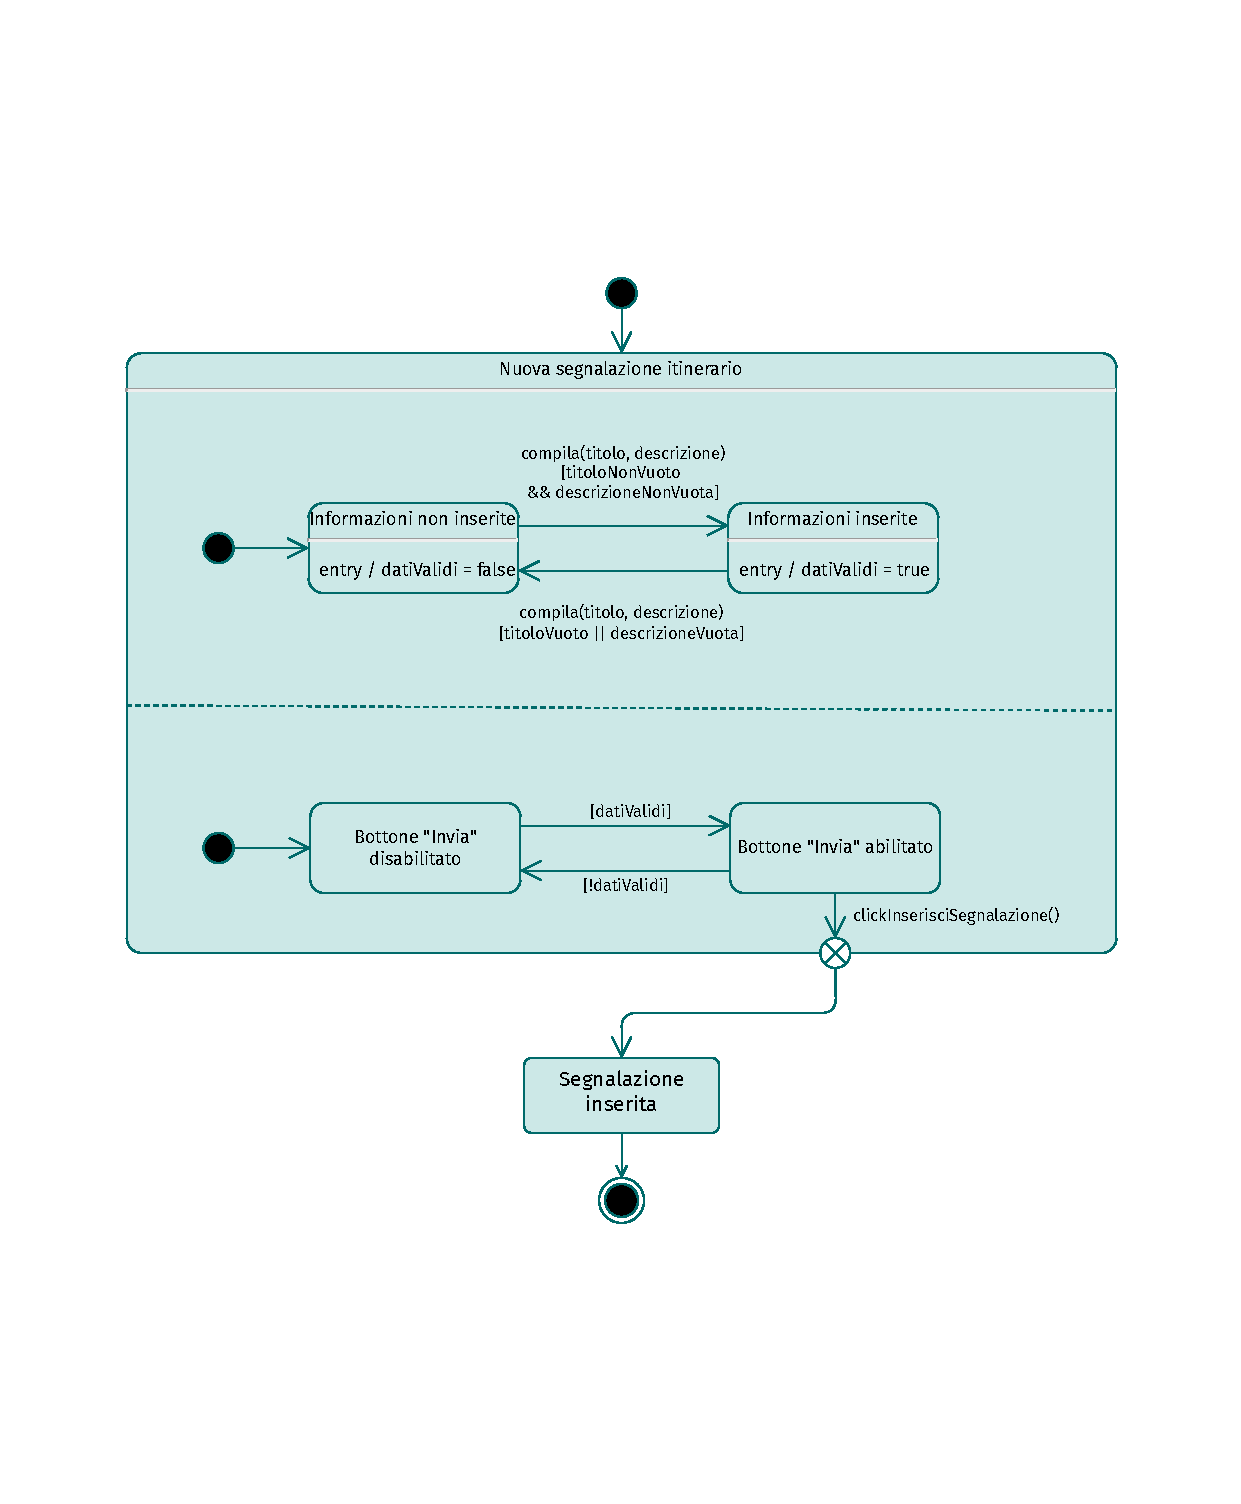
\includegraphics[width=\textwidth, page=1]{./diagrams/statechart.pdf}
	\caption{Nuova segnalazione itinerario}
\end{figure}
\FloatBarrier

\newpage
\subsubsection{Inserimento itinerario}
Per garantire una maggiore leggibilità, data l'estensione di questo statechart,
si è fatta la scelta di rappresentarlo tramite regioni interne, riportate poi per intero.
\begin{figure}[!htbp]
	\centering
	\includegraphics[width=\textwidth, page=2]{./diagrams/statechart.pdf}
	\caption{Nuovo itinerario}
\end{figure}
\FloatBarrier

\newpage
\begin{figure}[!htbp]
	\centering
	\includegraphics[width=\textwidth, page=3]{./diagrams/statechart.pdf}
	\caption{Regione interna - Inserimento dettagli itinerario}
\end{figure}
\FloatBarrier

\newpage
\begin{figure}[!htbp]
	\centering
	\includegraphics[width=\textwidth, page=4]{./diagrams/statechart.pdf}
	\caption{Regione interna - Inserimento mappa itinerario}
\end{figure}
\FloatBarrier

\newpage
\begin{figure}[!htbp]
	\centering
	\includegraphics[width=\textwidth, page=5]{./diagrams/statechart.pdf}
	\caption{Regione interna - Inserimento foto itinerario}
\end{figure}
\FloatBarrier

\newpage
\subsection{Classi, oggetti e relazioni di analisi}
Nella sezione seguente sono riportati i diagrammi di analisi \textbf{Entity Control Boundary}, un pattern architetturale \Gls{use-case driven}.

\subsubsection{Autenticazione}
\begin{figure}[!htbp]
	\centering
	\includesvg[width=\textwidth, height=21cm]{./diagrams/ecb/Login_+_Login_Social.svg}
	\caption{Login e login con social}
\end{figure}
\FloatBarrier

\begin{figure}[!htbp]
	\centering
	\includesvg[width=\textwidth, height=21cm]{./diagrams/ecb/Registrazione.svg}
	\caption{Registrazione e conferma}
\end{figure}
\FloatBarrier

\begin{figure}[!htbp]
	\centering
	\includesvg[width=\textwidth, height=21cm]{./diagrams/ecb/Password_dimenticata.svg}
	\caption{Password dimenticata}
\end{figure}
\FloatBarrier

\newpage
\begin{figure}[!htbp]
	\centering
	\includesvg[width=\textwidth, height=21cm]{./diagrams/ecb/Logout.svg}
	\caption{Logout}
\end{figure}
\FloatBarrier

\newpage

\subsubsection{Interazione con un itinerario}
\begin{figure}[!htpb]
	\centering
	\includesvg[width=\textwidth, height=21cm]{./diagrams/ecb/Aggiungi_itinerario.svg}
	\caption{Aggiunta itinerario}
\end{figure}
\FloatBarrier

\newpage

\begin{figure}[!htpb]
	\centering
	\includesvg[width=\textwidth, height=21cm]{./diagrams/ecb/Dettagli_itinerario.svg}
	\caption{Dettagli itinerario}
\end{figure}
\FloatBarrier

\newpage

\begin{figure}[!htpb]
	\centering
	\includesvg[width=\textwidth, height=21cm]{./diagrams/ecb/Elimina_Itinerario.svg}
	\caption{Eliminazione itinerario personale - Eliminazione itinerario altrui (admin)}
\end{figure}
\FloatBarrier

\newpage

\begin{figure}[!htpb]
	\centering
	\includesvg[width=\textwidth, height=21cm]{./diagrams/ecb/Ricerca_itinerario.svg}
	\caption{Ricerca itinerario}
\end{figure}
\FloatBarrier

\newpage

\begin{figure}[!htpb]
	\centering
	\includesvg[width=\textwidth, height=21cm]{./diagrams/ecb/Segnala_itinerario.svg}
	\caption{Segnalazione itinerario}
\end{figure}
\FloatBarrier

\newpage

\begin{figure}[!htpb]
	\centering
	\includesvg[width=\textwidth, height=21cm]{./diagrams/ecb/Valuta_itinerario.svg}
	\caption{Valuta itinerario}
\end{figure}
\FloatBarrier

\newpage

\subsubsection{Interazione con un post}
\begin{figure}[!htpb]
	\centering
	\includesvg[width=\textwidth, height=21cm]{./diagrams/ecb/Crea_Post.svg}
	\caption{Aggiunta post}
\end{figure}
\FloatBarrier

\newpage

\begin{figure}[!htpb]
	\centering
	\includesvg[width=\textwidth, height=21cm]{./diagrams/ecb/Dettagli_post.svg}
	\caption{Dettagli post}
\end{figure}
\FloatBarrier

\begin{figure}[!htpb]
	\centering
	\includesvg[width=\textwidth, height=21cm]{./diagrams/ecb/Segnala_post.svg}
	\caption{Segnala post}
\end{figure}
\FloatBarrier

\begin{figure}[!htpb]
	\centering
	\includesvg[width=\textwidth, height=21cm]{./diagrams/ecb/Rimuovi_Post.svg}
	\caption{Eliminazione post personale}
\end{figure}
\FloatBarrier

\newpage

\subsubsection{Interazione con una compilation}
\begin{figure}[!htpb]
	\centering
	\includesvg[width=\textwidth, height=21cm]{./diagrams/ecb/Crea_compilation.svg}
	\caption{Aggiunta compilation}
\end{figure}
\FloatBarrier

\newpage

\begin{figure}[!htpb]
	\centering
	\includesvg[width=\textwidth, height=21cm]{./diagrams/ecb/Dettaglio_compilation_+_Elimina_itinerario_da_compilation.svg}
	\caption{Dettagli compilation e rimozione itinerario da compilation}
\end{figure}
\FloatBarrier

\newpage

\begin{figure}[!htpb]
	\centering
	\includesvg[width=\textwidth, height=21cm]{./diagrams/ecb/Salva_itinerario_in_compilation.svg}
	\caption{Salvataggio itinerario in compilation}
\end{figure}
\FloatBarrier

\newpage

\begin{figure}[!htpb]
	\centering
	\includesvg[width=\textwidth, height=21cm]{./diagrams/ecb/Elimina_compilation.svg}
	\caption{Eliminazione compilation personale}
\end{figure}
\FloatBarrier

\newpage

\subsubsection{Gestione profilo e interazione con gli utenti}
\begin{figure}[!htpb]
	\centering
	\includesvg[width=\textwidth, height=21cm]{./diagrams/ecb/Storico_conversazioni_+_Invia_messaggio.svg}
	\caption{Storico conversazioni e invio messaggio privato}
\end{figure}
\FloatBarrier

\begin{figure}[!htpb]
	\centering
	\includesvg[width=\textwidth, height=21cm]{./diagrams/ecb/Ricerca_destinatario_messaggio.svg}
	\caption{Ricerca destinatario messaggio}
\end{figure}
\FloatBarrier

\begin{figure}[!htpb]
	\centering
	\includesvg[width=\textwidth, height=21cm]{./diagrams/ecb/Aggiorna_foto_profilo.svg}
	\caption{Aggiornamento foto profilo}
\end{figure}
\FloatBarrier

\newpage

\subsubsection{Funzionalità riservate agli amministratori}
\begin{figure}[!htpb]
	\centering
	\includesvg[width=\textwidth, height=21cm]{./diagrams/ecb/modifica_adm_itinerario.svg}
	\caption{Modifica itinerario}
\end{figure}
\FloatBarrier

\newpage

\begin{figure}[!htpb]
	\centering
	\includesvg[width=\textwidth, height=21cm]{./diagrams/ecb/dettagli-segnalazione.svg}
	\caption{Dettagli segnalazione e eliminazione segnalazione}
\end{figure}
\FloatBarrier


\newpage
\subsection{Diagrammi di sequenza di analisi}
Sono presentati nella seguente sezione i Sequence Diagram relativi a due funzionalità offerte dall'applicazione:
la segnalazione di un itinerario e la ricerca di un itinerario.
\subsubsection{Segnalazione itinerario}
\begin{figure}[!htbp]
	\centering
	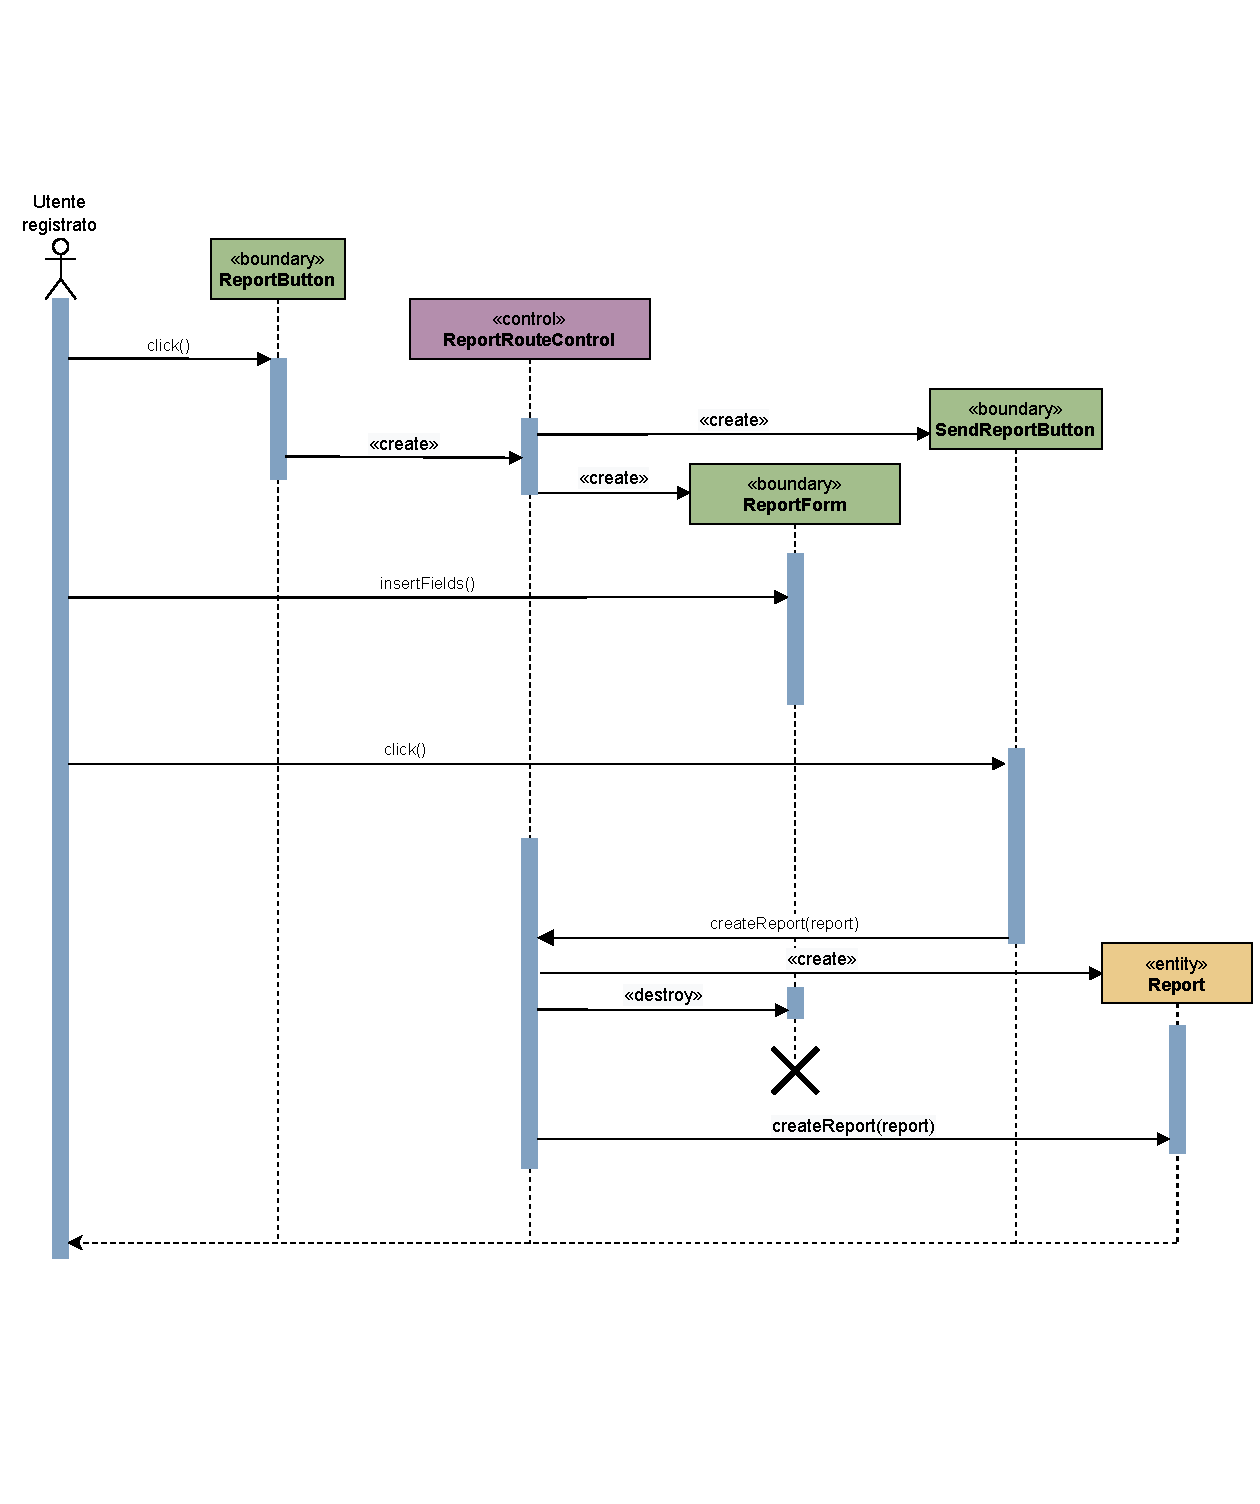
\includegraphics[width=\textwidth, page=1]{./diagrams/sequenceDomain-segnalazioneItinerario.pdf}
	\caption{Sequence Diagram 1 - Segnalazione di un itinerario}
\end{figure}
\FloatBarrier

\newpage
\subsubsection{Ricerca itinerario}
\begin{figure}[!htbp]
	\centering
	\includesvg[width=\textwidth, height=21cm]{./diagrams/sequenceDomain-ricercaItinerario.svg}
	\caption{Sequence Diagram 2 - Ricerca di un itinerario}
\end{figure}
\FloatBarrier

\newpage
\subsection{Diagrammi di attività}
\subsubsection{Autenticazione}
\begin{figure}[!htbp]
	\centering
	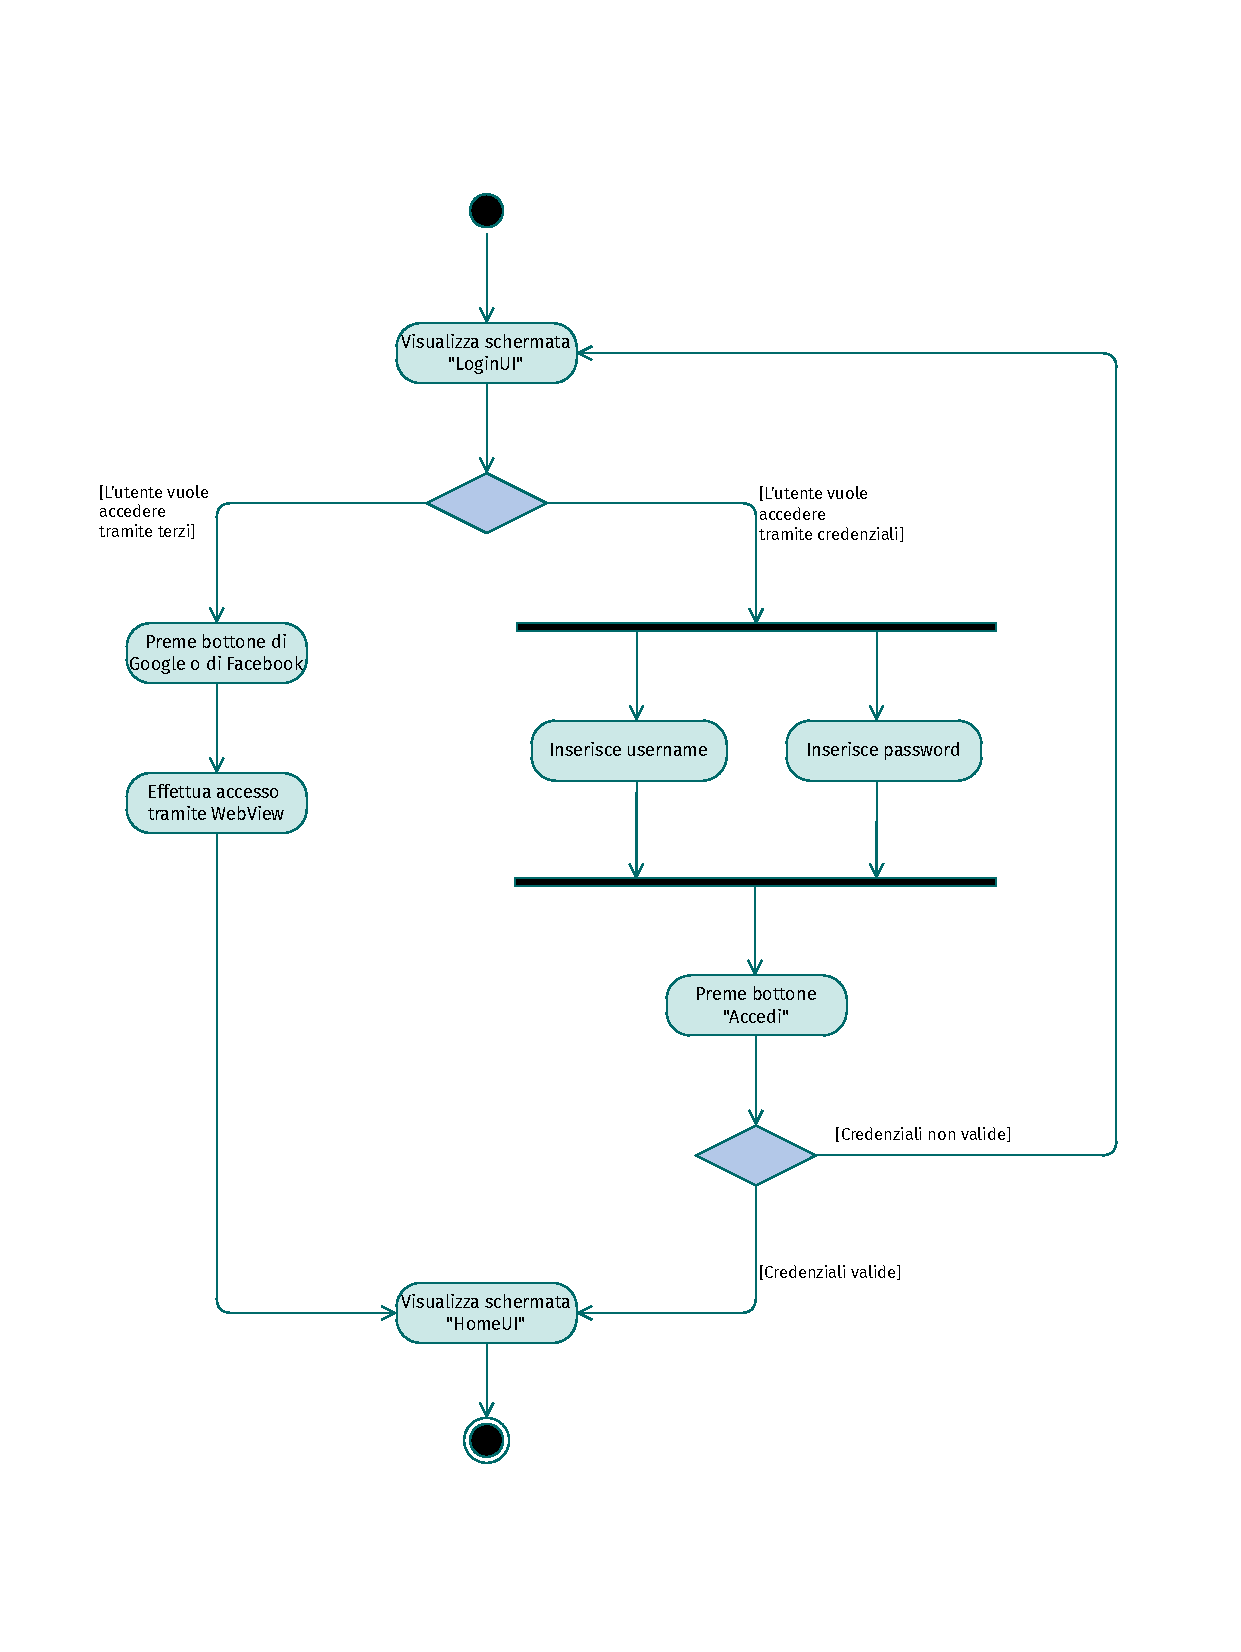
\includegraphics[width=\textwidth, page=1]{./diagrams/activity.pdf}
	\caption{Login utente}
\end{figure}
\FloatBarrier

\newpage
\begin{figure}[!htbp]
	\centering
	\includesvg[width=\textwidth, height=21cm]{./diagrams/activity-registrazione.svg}
	\caption{Registrazione utente}
\end{figure}
\FloatBarrier

\newpage
\begin{figure}[!htbp]
	\centering
	\includesvg[width=\textwidth, height=21cm]{./diagrams/activity-forgot_password.svg}
	\caption{Reset password dimenticata}
\end{figure}
\FloatBarrier

\newpage
\begin{figure}[!htbp]
	\centering
	\includegraphics[width=\textwidth, page=16]{./diagrams/activity.pdf}
	\caption{Logout}
\end{figure}
\FloatBarrier


\newpage
\subsubsection{Interazione con un itinerario}
\begin{figure}[!htbp]
	\centering
	\includesvg[width=\textwidth, height=21cm]{./diagrams/activity_aggiungi_itinerario.svg}
	\caption{Aggiunta itinerario}
\end{figure}
\FloatBarrier

\newpage
\begin{figure}[!htbp]
	\centering
	\includegraphics[width=\textwidth, page=9]{./diagrams/activity.pdf}
	\caption{Rimozione itinerario}
\end{figure}
\FloatBarrier

\newpage
\begin{figure}[!htbp]
	\centering
	\includegraphics[width=\textwidth, page=2]{./diagrams/activity.pdf}
	\caption{Ricerca itinerario}
\end{figure}
\FloatBarrier

\newpage
\begin{figure}[!htbp]
	\centering
	\includegraphics[width=\textwidth, page=10]{./diagrams/activity.pdf}
	\caption{Valutazione itinerario}
\end{figure}
\FloatBarrier

\newpage
\begin{figure}[!htbp]
	\centering
	\includegraphics[width=\textwidth, page=11]{./diagrams/activity.pdf}
	\caption{Salvataggio itinerario}
\end{figure}
\FloatBarrier

\newpage
\begin{figure}[!htbp]
	\centering
	\includegraphics[width=\textwidth, page=12]{./diagrams/activity.pdf}
	\caption{Segnalazione itinerario}
\end{figure}
\FloatBarrier

\newpage
\subsubsection{Interazione con un post}
\begin{figure}[!htbp]
	\centering
	\includegraphics[width=\textwidth, page=3]{./diagrams/activity.pdf}
	\caption{Aggiunta post}
\end{figure}
\FloatBarrier

\newpage
\begin{figure}[!htbp]
	\centering
	\includegraphics[width=\textwidth, page=4]{./diagrams/activity.pdf}
	\caption{Rimozione post}
\end{figure}
\FloatBarrier

\newpage
\begin{figure}[!htbp]
	\centering
	\includegraphics[width=\textwidth, page=14]{./diagrams/activity.pdf}
	\caption{Segnalazione post}
\end{figure}
\FloatBarrier

\newpage
\subsubsection{Interazione con una compilation}
\begin{figure}[!htbp]
	\centering
	\includegraphics[width=\textwidth, page=7]{./diagrams/activity.pdf}
	\caption{Aggiunta compilation}
\end{figure}
\FloatBarrier

\newpage
\begin{figure}[!htbp]
	\centering
	\includegraphics[width=\textwidth, page=9]{./diagrams/activity.pdf}
	\caption{Rimozione compilation}
\end{figure}
\FloatBarrier

\newpage
\begin{figure}[!htbp]
	\centering
	\includegraphics[width=\textwidth, page=8]{./diagrams/activity.pdf}
	\caption{Rimozione itinerario da compilation}
\end{figure}
\FloatBarrier

\newpage
\subsubsection{Gestione profilo e interazione con utenti}
\begin{figure}[!htbp]
	\centering
	\includegraphics[width=\textwidth, page=16]{./diagrams/activity.pdf}
	\caption{Invio messaggio}
\end{figure}
\FloatBarrier

\begin{figure}[!htbp]
	\centering
	\includegraphics[width=\textwidth, page=17]{./diagrams/activity.pdf}
	\caption{Ricerca destinatario messaggio}
\end{figure}
\FloatBarrier

\newpage
\begin{figure}[!htbp]
	\centering
	\includegraphics[width=\textwidth, page=15]{./diagrams/activity.pdf}
	\caption{Avvio conversazione con l'autore di un post o itinerario}
\end{figure}
\FloatBarrier

\newpage
\begin{figure}[!htbp]
	\centering
	\includegraphics[width=\textwidth, page=5]{./diagrams/activity.pdf}
	\caption{Modifica foto profilo}
\end{figure}
\FloatBarrier

\newpage
\subsubsection {Funzionalità riservate agli amministratori}
\begin{figure}[!htbp]
	\centering
	\includegraphics[width=\textwidth, page=18]{./diagrams/activity.pdf}
	\caption{Rimozione segnalazione}
\end{figure}
\FloatBarrier

\newpage
\begin{figure}[!htbp]
	\centering
	\includegraphics[width=\textwidth, page=19]{./diagrams/activity.pdf}
	\caption{Modifica itinerario}
\end{figure}
\FloatBarrier

\newpage
\section{Documento di Design del sistema}
\subsection{Analisi dell'architettura e criteri di design}
\subsubsection{Diagramma di design del sistema}
In questa sezione viene presentato un diagramma realizzato con lo scopo di
rappresentare la struttura generale dell'architettura di sistema realizzata;
in esso sono stati messi in evidenza i servizi di cui si è usufruito nello sviluppo del software. \\
Le specifiche di ciascuna scelta implementativa sono
dettagliate nelle sezioni successive.
\begin{figure}[!htbp]
	\centering
	\includegraphics[width=\textwidth]{./diagrams/sysdesign.pdf}
	\caption{Diagramma del sistema}
\end{figure}

\newpage
\subsubsection{Software deployment}
L'architettura del software realizzato pone le sue fondamenta nel concetto di \textbf{cloud computing}.\\
Il cloud computing, o computazione cloud, consiste nella distribuzione on-demand di risorse IT, con
una tariffazione basata sul consumo.\\\\
Tra i diversi provider, è stato scelto di usufruire dei servizi offerti dalla piattaforma proprietaria del gruppo
Amazon \textbf{AWS}, \textbf{Amazon Web Services}.
AWS offre infatti cloud services ideali per creare applicazioni in modo scalabile, flessibile e affidabile; esso
presenta inoltre notevoli vantaggi, ritenuti come caratteristiche desiderabili per la progettazione di qualunque software.\\

La scelta della piattaforma AWS è stata compiuta, inoltre, per le seguenti qualità:
\begin{itemize}
	\item \textbf{Agilità} - la possibilità di aumentare a seconda delle necessità risorse quali servizi infrastrutturali,
	      calcolo, storage e database;
	\item \textbf{Elasticità} - la possibilità di evitare l'allocazione anticipata di una quantità maggiore di risorse di
	      quante siano necessarie, così da gestire i picchi nei livelli di attività future;
	\item \textbf{Distribuzione globale di contenuti} - l'infrastruttura AWS offre una copertura globale: fare in modo che le
	      applicazioni siano vicino agli utenti finali riduce la latenza e migliora la loro esperienza.\\
\end{itemize}


AWS offre una grande varietà di servizi; ciascuno di essi va incontro a una specifica necessità dello sviluppatore. \\
Nello sviluppo del software, per implementare determinate funzionalità si è scelto di ricorrere all'utilizzo dei seguenti servizi:
\begin{itemize}
	\item \textbf{Cognito} - Amazon Cognito permette di aggiungere strumenti di registrazione degli utenti, accesso
	      e controllo degli accessi alle app Web e per dispositivi mobili. Esso supporta l'accesso degli utenti
	      tramite l'uso di provider di identità social quali Facebook, Google.
	      Tale risorsa è stata sfruttata realtivamente all'autenticazione utente, tenendo particolarmente in considerazione
	      l'alto fattore di sicurezza che essa conferisce;
	\item \textbf{EC2} - l'\textbf{Elastic Compute Cloud} (Amazon EC2) fornisce capacità di calcolo scalabile in AWS Cloud.
	      Esso offre ambienti di elaborazione virtuale, noti come \textit{istanze}, varie configurazioni di CPU, memoria,
	      archiviazione e capacità di rete per le istanza note come \textit{tipi di istanza}.
	      La scelta di tale servizio è stata finalizzata al \Gls{deploy} dell'applicativo Spring, nella realizzazione del \Gls{REST} Service.
	\item \textbf{RDS} - Amazon RDS ha permesso la configurazione e l'utilizzo del database relazionale alla base del software prodotto;
	\item \textbf{S3} - il \textbf{Simple Storage Service} (Amazon S3) permette l'archiviazione di oggetti in modo scalabile.
	      Esso è stato adoperato in merito alla preservazione permanente dei file immagine caricati dagli utenti;
	\item \textbf{Lambda} - AWS Lambda è un servizio di calcolo basato su eventi serverless.
	      La scelta del servizio Lambda è stata incentivata dalla sua possibilità di integrazione con il servizio \textbf{Cognito}, e dettata
	      dalla volontà di conferire \textit{consistenza} al pool utenti del sistema.
	      Nello specifico, si è sfruttata la possibilità offerta dal servizio di creare dei \textit{trigger} (in particolare trigger di \textit{post conferma}), al fine di
	      evitare - in seguito al processo di registrazione - la possibile presenza di inconsistenze tra database e registrazioni effettivamente portate a termine.
\end{itemize}

Si è ritenuto inoltre fondamentale l'utilizzo del framework \textbf{Amplify}.\\
In particolare, Amplify è stato impiegato per realizzare:
\begin{itemize}
	\item Un servizio di autenticazione particolarmente sicuro tramite, come citato, il servizio \textit{Cognito};
	\item L'archiviazione di file (nella prima versione del software solo di file immagine) tramite il servizio \textit{S3}.
\end{itemize}

È importante specificare che il framework Amplify consente anche di creare back-end o applicativi serverless. Ciononostante, si sottolinea che
nella realizzazione del software è stata fatta la scelta di utilizzarlo \textit{solo} in funzione dei servizi da essi offerti, soprattutto in relazione alla deprecazione
dell'SDK standard AWS per Android.

\subsubsection{Google Maps Platform}
Una delle caratteristiche principali del software risulta essere la forte componente geolocalizzata degli itinerari presenti in piattaforma. \\
Gli utenti, infatti, nell'inserimento e nella visualizzazione dei sentieri si trovano ad interfacciarsi direttamente con mappe interattive.
Per garantire un'esperienza ottimale da questo punto di vista sono stati utilizzati i servizi della piattaforma Google Maps. \\\\
La \textbf{Google Maps Platform} è un insieme di API e SDK che permette di integrare in applicazioni mobile Google Maps, e di recuperare dati da esso stesso.
L'esperienza utente con le funzionalità sopracitate è stata supportata dall'utilizzo delle seguenti API:
\begin{itemize}
	\item MapsAPI - per la visualizzazione interattiva di mappe statiche e dinamiche;
	\item PlacesAPI - per il recupero di informazioni sui posti tramite richieste HTTP;
	\item DirectionsAPI - per il calcolo del percorso tra diverse tappe; utilizzano una richiesta HTTP per ritornare le direzioni tra località in formato JSON o XML.
	      Le DirectionsAPI, in quanto web service, sono state integrate nel Rest Service proprio del software.
\end{itemize}

\subsubsection{Architettura del REST Service}
Nella realizzazione del REST Service è stato scelto di utilizzare il framework \textbf{Spring}. \\
Spring fornisce un'\textit{infrastruttura di supporto} per lo sviluppo di applicazioni: esso prevede una \textit{modularizzazione} dell'architettura come segue:
\begin {itemize}
\item Presentation layer - strato più esterno, che gestisce la presentazione del contenuto e l'interazione con l'utente;
\item Business logic layer - strato centrale, che gestisce la logica;
\item Data access layer - strato più interno, che gestisce il recupero di dati dalle diverse sorgenti.
\end{itemize}

Ciascuno di questi strati dipende da quello sottostante per far sì che l'applicazione funzioni. In altre parole,
lo strato di presentazione comunica con quello della business logic, che a sua volta comunica con lo strato di data
access. Ogni strato ha quindi bisogno di questa \textit{dipendenza} per eseguire il proprio compito correttamente \\

La scelta di utilizzare il framework Spring è stata fatta in relazione alla volontà di ottenere un \textit{loose coupling}, ossia un accoppiamento largo.
Senza l'utilizzo di Spring, ci sarebbe stata la possibilità che il codice avesse potuto causare \textit{tight coupling}, che non è
considerato essere una buona pratica di programmazione. Il loose coupling è ideale, in quanto le componenti largamente
accoppiate sono indipendenti: ciò implica che, a seguito di possibili cambiamenti futuri, questi non influenzeranno
le altre componenti.\\

Al cuore del framework Spring si trova la \textbf{dependency injection}. \\
La dependency injection è un pattern di programmazione che permette agli sviluppatori di costruire architetture disaccoppiate. Ciò vuol dire che Spring comprende le \textit{annotazioni}
poste in capo alle classi; in seguito alla creazione di un'istanza, dunque, il framework si assicura che le istanze siano state create con le opportune dependencies. \\\

Nello specifico, per l'implementazione del software, è stata utilizzata un'estensione del framework Spring, chiamata \textbf{Spring Boot}.\\
Spring Boot ha delle caratteristiche specifiche che rendono la gestione dell'applicazione più semplice.\\
Tra alcuni dei vantaggi che hanno portato alla scelta di Spring Boot, si ricordano:
\begin{itemize}
	\item Creazione di applicazioni Spring stand-alone;
	\item Dotazione di dependencies "starter" per semplificare la configurazione di build;
	\item Configurazione automatica di Spring e di librerie di terze parti, ove possibile;
	\item Nessuna generazione di codice e nessun requisito per la configurazione XML;
	\item Inclusione di un web server embedded (nello specifico \textit{Apache Tomcat}) senza la necessità di ulteriori configurazioni.
\end{itemize}

\newpage
Di seguito viene presentato un diagramma che dettaglia la struttura e il funzionamento del REST Service.
\begin{figure}[!htbp]
	\centering
	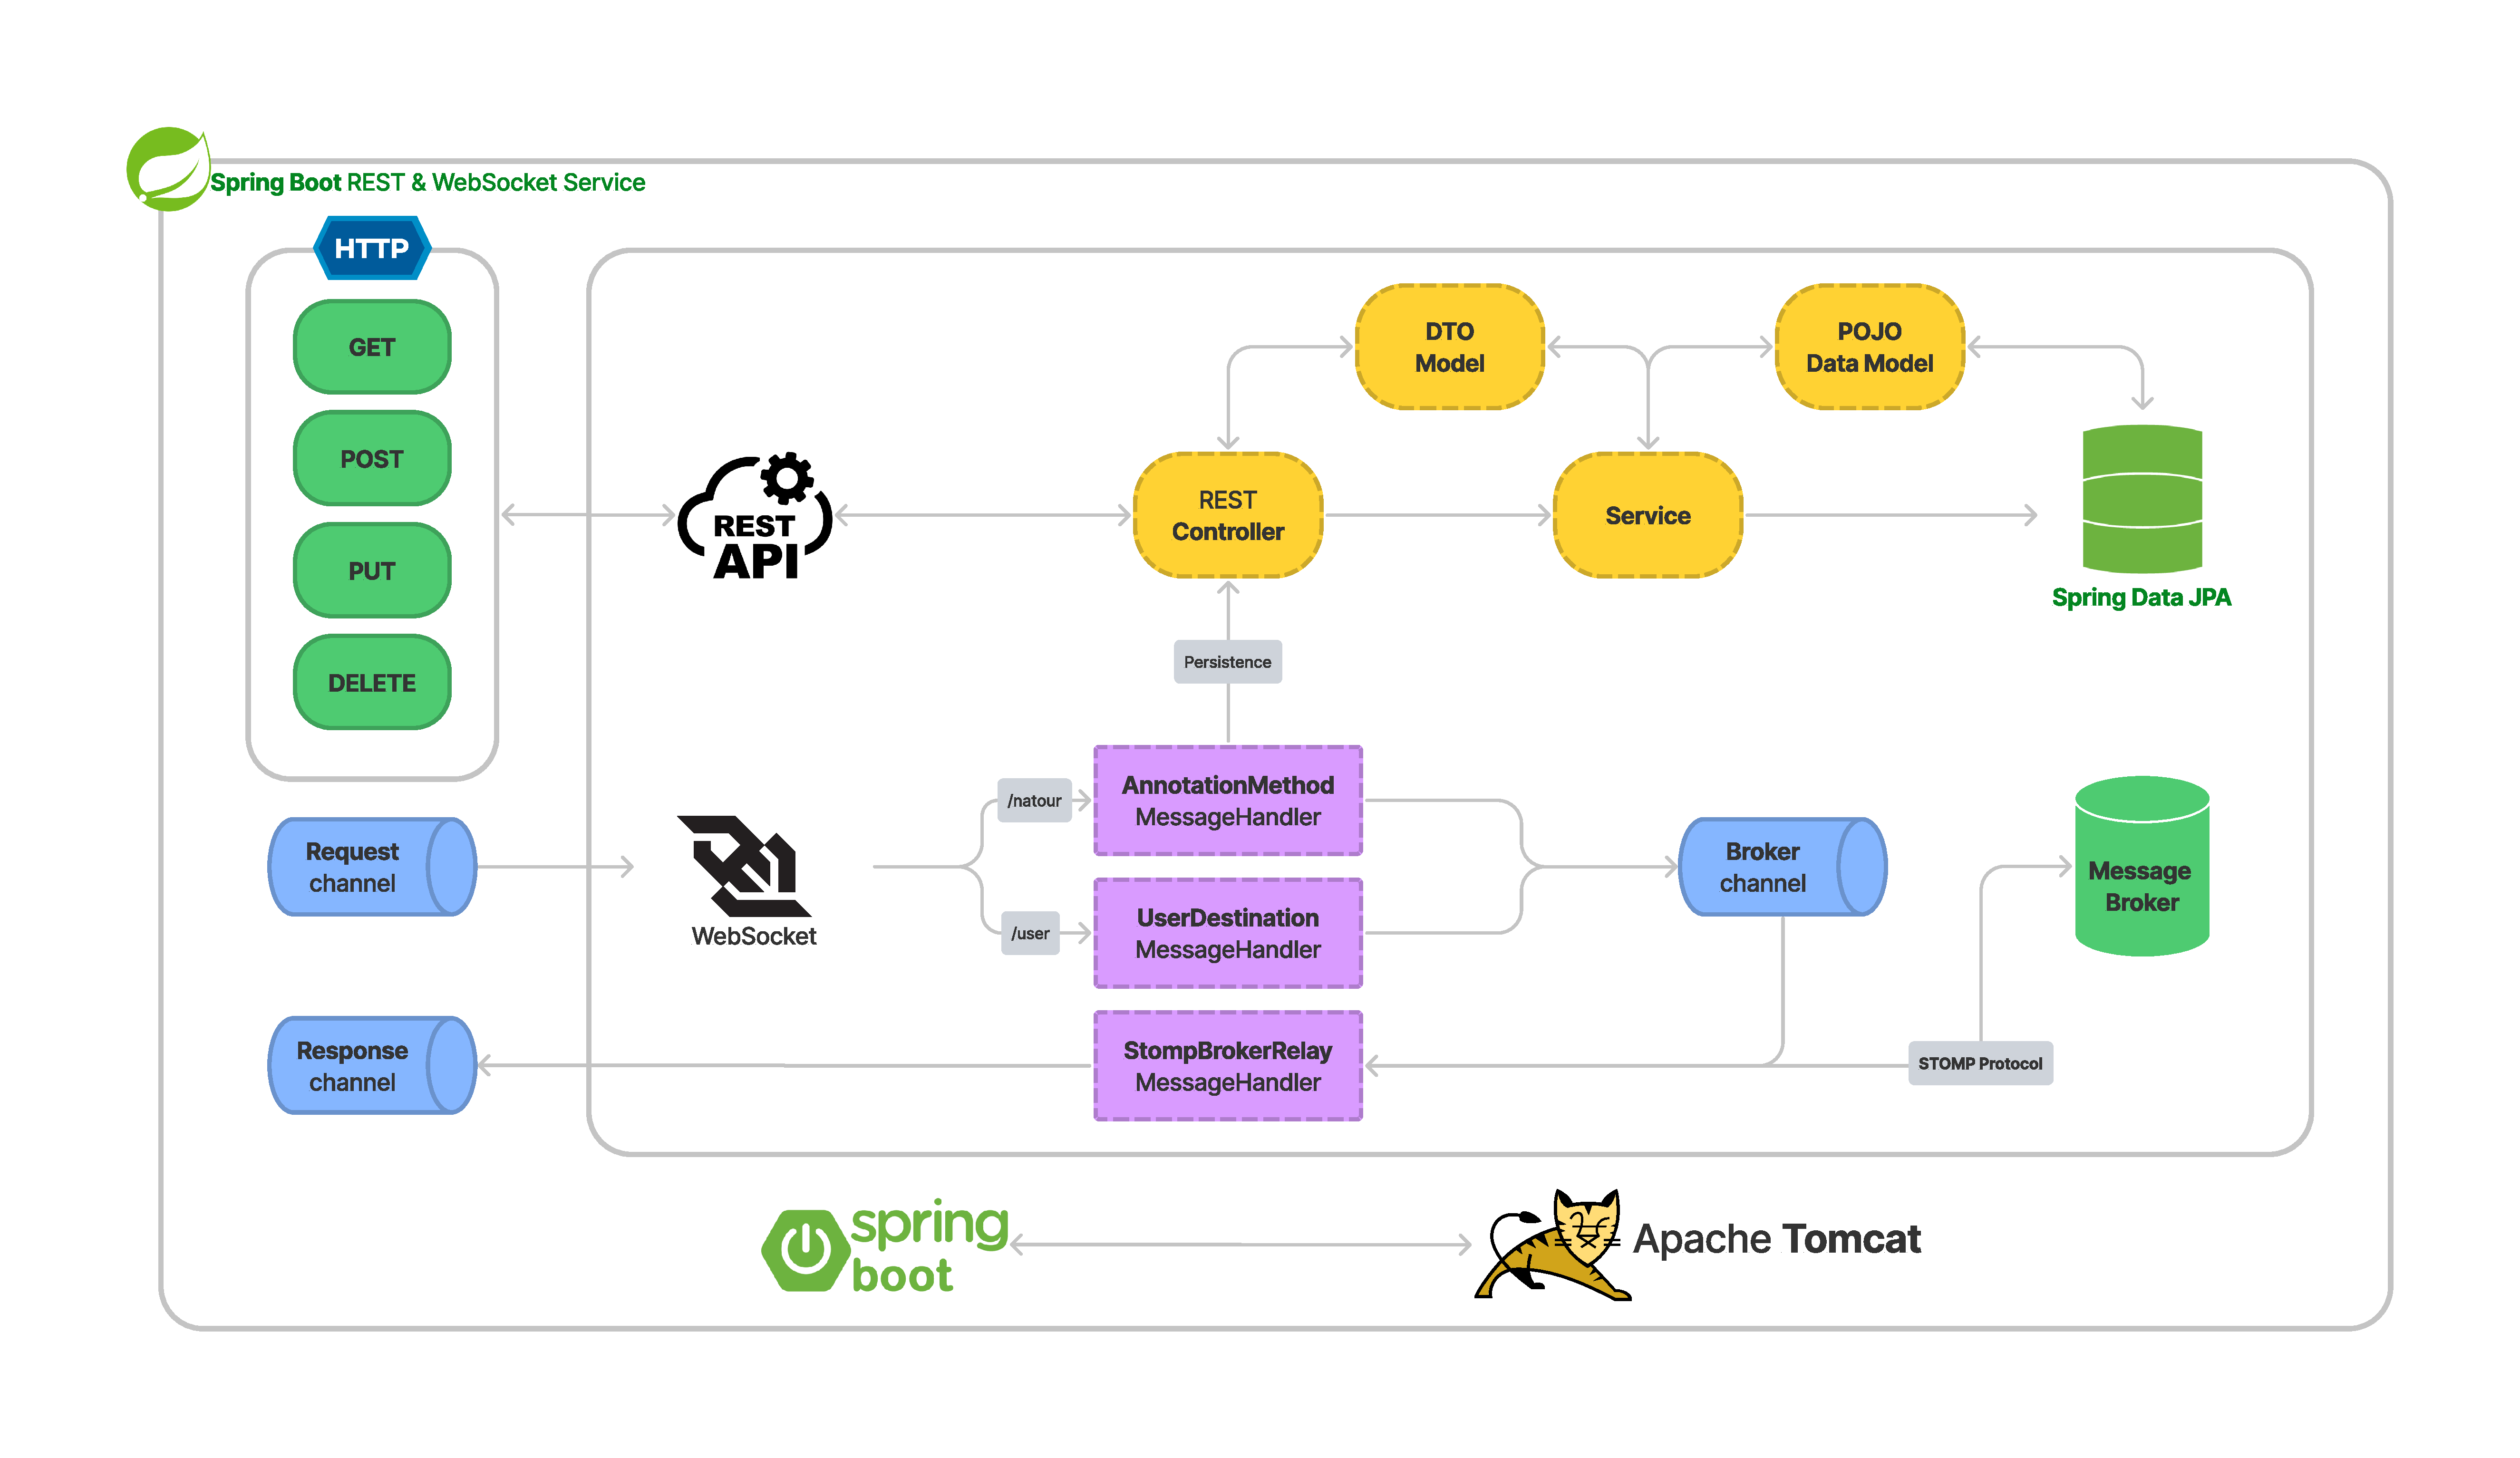
\includegraphics[width=\textwidth]{./diagrams/spring.pdf}
	\caption{REST + WS Service realizzato con Spring Boot}
\end{figure}

\newpage
\subsection{Architettura dell’applicativo}
L'intera architettura del software è stata progettata seguendo le linee guida della cosiddetta \textbf{Clean Architecture}. \\
Il concetto di architettura \textit{pulita} si basa sui principi enunciati da Robert C. Martin nel libro "Clean Architecture".
In seguito alle informazioni acquisite dalla lettura del libro, infatti, questo approccio è stato ritenuto quello più valido.\\
L’idea chiave è quella di utilizzare il principio di inversione di dipendenza per porre dei boundaries tra componenti di alto livello e componenti di basso livello.
Ciò crea un’architettura \textit{plug-in},
che conferisce al sistema un’elevata flessibilità e un'elevata manutenibilità. \\
Un’architettura \textit{pulita} inizia da un codice \textit{pulito}. Classi pulite derivano da componenti pulite, che, a loro volta, determinano un \textit{sistema pulito}.\\
È stato quindi ritenuto di fondamentale importanza applicare i principi della Clean Architecture e del Clean Code in maniera uniforme e costante, nell'implementazione di qualsiasi componente.\\

\begin{figure}[!htbp]
	\centering
	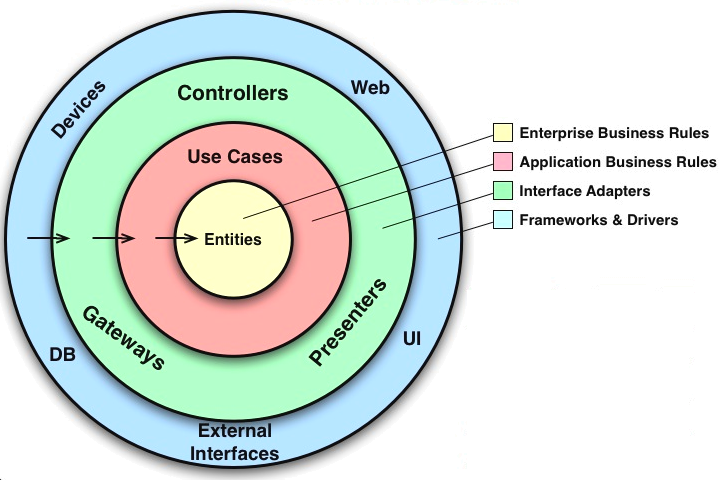
\includegraphics[width=\textwidth]{./diagrams/cleanarchitecture.png}
	\caption{Clean Architecture}
\end{figure}

Il concetto di \textit{Clean Code} sfruttato nello sviluppo del software segue i principi \textbf{SOLID}. \\
Tali principi sono stati applicati in modo da ottimizzare l’architettura e ciascuna delle sue componenti, le quali risultano dunque essere caratterizzate dal:
\begin{itemize}
	\item \textbf{Single responsability principle} – una classe dovrebbe avere uno ed un solo motivo per cambiare;
	\item \textbf{Open-closed principle} – una classe dovrebbe essere aperta all’estensione ma chiusa alle modifiche;
	\item \textbf{Liskov’s substitution principle} – gli oggetti di un programma dovrebbero essere sostituibili con istanze dei propri sottotipi senza alterare la correttezza del programma stesso;
	\item \textbf{Interface segregation principle} – più interfacce client-specific sono meglio di un’unica interfaccia general-purpose;
	\item \textbf{Dependency inversion principle}\footnote{
		      Il principio di inversione di dipendenza è stato applicato, in particolare, in relazione agli UseCase (nel Domain Layer): la loro indipendenza dagli altri moduli fa in modo che essi possano dipendere
		      solo da \textit{astrazioni} dei loro strati.}
	      – i moduli di alto livello non dovrebbero dipendere da moduli di basso livello; entrambi dovrebbero dipendere da \textit{astrazioni}.
\end{itemize}

Il concetto di Clean Architecture si basa sulla \textit{modularità} dell’architettura stessa. \\
Nel caso della progettazione del software prodotto è stata seguita una suddivisione del seguente tipo:
\begin{itemize}
	\item Presentation layer – responsabile della presentazione a schermo e della gestione delle
	      interazioni degli utenti;
	\item Domain layer – rappresentazione formale del dominio applicativo
	\item Data layer – contenitore delle implementazioni delle sorgenti di dati e dei repository,
	      i quali coordinano i dati provenienti da esse.
\end{itemize}

È bene sottolineare, però, che nell'effettiva implementazione dell'applicativo non è
stato pedissequamente seguito lo schema appena proposto. \\
È stato ritenuto più opportuno adottare un approccio \textit{per funzionalità}; ciò è risultato nell'applicazione del concetto di \textbf{Screaming Architecture.} Di seguito ne
è mostrato un esempio di implementazione, tratto dal software stesso. \\
\begin{figure}[!htbp]
	\centering
	\includegraphics{./diagrams/design/screaming.png}
\end{figure}
\FloatBarrier
L'espressione "Screaming Architecture" è stata coniata dal sopracitato Robert C. Martin; essa viene utilizzata nelle situazioni in cui,
rivolgendo un solo sguardo ad un progetto, si riesce ad avere un'idea di base su cosa esso faccia e su cosa riguardi. \\
Da ciò deriva la possibilità di comprendere esattamente la struttura al cuore del codice implementato:
la suddivisione nei diversi package "urla" al lettore l'approccio utilizzato, che risulta dunque chiaro e comprensibile già a primo impatto.\\


La Clean Architecture non preclude, però, la possibilità di adattare all'applicativo un proprio design pattern architetturale. \\
Come descritto nella sezione successiva, tale approccio è stato ritenuto adatto alle esigenze di implementazione.

\newpage

\subsection{Le scelte implementative}
\subsubsection{Applicazioni mobile native e ibride}
Un’applicazione mobile nativa è un’applicazione software sviluppata per funzionare su uno specifico tipo di dispositivo o piattaforma.
Le app native consentono performance migliori, un’esecuzione veloce e un alto grado di precisione. Ciononostante, esse presentano alcune problematiche:
\begin{itemize}
	\item Le app native richiedono codice sorgente \textit{esclusivo}, poiché ogni dispositivo deve avere la sua versione specifica dell’app;
	\item Richiedono un costo maggiore, e sono richiesti più sviluppatori per creare e gestire il codice per ogni piattaforma;
	\item È richiesto molto tempo per la creazione differenziata per i diversi sistemi operativi in ogni aggiornamento delle funzionalità.
\end{itemize}

Le app ibride combinano gli elementi di applicazioni web e native; i linguaggi utilizzati fanno parte di tecnologie web come HTML, CSS e JavaScript.
\begin{itemize}
	\item Hanno un’interfaccia utente multipiattaforma;
	\item Possono essere sviluppate più velocemente e richiedono meno costi di sviluppo e manutenzione;
	\item Non hanno bisogno di codice sorgente specifico.
	\item Penalizzano la UX in alcuni casi.
\end{itemize}

La scelta stata è influenzata da diversi fattori. Tra i requisiti del sistema sono richieste prestazioni di buon livello, e il target
di clienti è particolarmente esigente.
È stato adottato un approccio nativo, precisamente su sistema operativo \textbf{Android}, scegliendo \textbf{Kotlin} come linguaggio di programmazione.

\subsubsection{Perchè Kotlin?}
Java detiene da anni un ruolo chiave nello sviluppo di applicazioni, tuttavia alcuni requisiti \textit{platform-dependant}
possono rendere tedioso l'utilizzo di questo linguaggio. Esistono altri linguaggi che operano sulla JVM: tra questi, Kotlin ha guadagnato
molti punti a favore nello sviluppo di applicazioni native Android. \\

Kotlin presenta molti vantaggi; tra essi si sottolineano:
\begin{itemize}
	\item Elevata \textbf{concisione}, raggiunta attraverso l'inferenza di tipi, lo \textit{smart-cast} e le \textit{data class}:
	      tali fattori conferiscono al codice una maggiore le leggibilità e manutenibilità. Ciò avviene anche in relazione al fatto che - sfruttando queste
	      tecnologie - il codice necessario per l'implementazione di una feature risulta essere di un numero di righe di gran lunga minore rispetto allo stesso codice sviluppato in Java; \\
	\item Il type system di Kotlin mira ad eliminare le \textit{NullPointerException}, garantendo controlli a tempo di compilazione e offrendo
	      operatori di \textit{null-safety}.
\end{itemize}

Tra le funzionalità più interessanti volte a migliorare la produttività dello sviluppatore è presenta una forte integrazione del paradigma di
programmazione funzionale, oltre alla possibilità di creare particolari funzioni note come \textit{estensioni}, che consentono l'aggiunta
di nuovi metodi a classi pre-esistenti.

Inoltre, Kotlin non preclude la possibilità di utilizzare codice Java, ma questa possibilità è bi-direzionale: Java e Kotlin possono coesistere
all'interno dello stesso progetto. \\

Alla luce delle informazioni fornite, Kotlin è stato ritenuto poter essere un valido alleato nello sviluppo dell'applicativo.

\newpage

\subsubsection{Diagramma di design dell'applicativo}
In questa sezione viene presentato un diagramma realizzato con lo scopo di rappresentare la struttura generale dell'applicativo. \\
Le specifiche di ciascuna scelta implementativa sono dettagliate nelle sezioni successive.
\begin{figure}[!htbp]
	\centering
	\includepdf[pages=1, height=17cm]{./diagrams/android.pdf}
\end{figure}

\newpage
\subsubsection{Pattern architetturale utilizzato}
Il design pattern architetturale potrebbe essere definito come \textit{ibrido}: ciò è dovuto alla
\textit{fusione} di due pattern differenti utilizzati nella progettazione. \\
Tali pattern sono \textbf{MVVM} e \textbf{MVI}; quest'ultimo è stato utilizzato per ovviare ai problemi
sofferti dal primo. Procediamo ad un'analisi più dettagliata. \\

\textbf{MVVM} è un'architettura del tipo Model-View-ViewModel che evita l'accoppiamento stretto
tra ciascuna componente. Più nello specifico, in questo tipo di architettura, i figli non hanno un
riferimento diiretto al padre, ma hanno solo riferimenti tramite \textit{observables}.\\
Esso è organizzato secondo tre strati:
\begin{itemize}
	\item Model - rappresenta i dati e la business logic dell'applicazione;
	\item View - consiste del codice relativo alle interfacce utente;
	\item ViewModel - definisce una sorta di ponte tra i due modelli sopracitati.
\end{itemize}

Il modello MVVM, per quanto affermato, pone però alcune problematiche, quali ad esempio:
\begin{itemize}
	\item la difficoltà di riusabilità sia per le View che per i ViewModel;
	\item la registrazione a molteplici observables nello stesso ViewModel, che ne aumenta le relative responsabilità;
	\item View e ViewModel possono essere soggetti ad avere un coupling stretto.
\end{itemize}

A questo scopo, è stata realizzata un'integrazione con il modello MVI, la cui differenza principale si risolve nell'assenza
della moltitudine di observables citati in precedenza. \\

\textbf{MVI} sta per Model-View-Intent. Si tratta di uno dei pattern architetturali più recenti per applicazioni Android.
\begin{itemize}
	\item Model - rappresenta uno stato. I Model dovrebbero essere immutabili, in modo da
	      assicurare un flow di dati unidirezionale con gli altri strati;
	\item View - rappresenta le View, che possono essere implementate in Activity o Fragment
	\item Intent - rappresenta un'intenzione o una volontà di eseguire un'azione, sia dell'utente
	      che dell'app stessa. Gli Intent si traducono in \textit{Event} ed \textit{Effect}.
\end{itemize}

L'integrazione dei due pattern architetturali sopracitati culmina nella nascita di un nuovo pattern, chiamato dagli sviluppatori Android \Gls{UDF}.\\
Alcune delle caratteristiche di UDF possono essere così sintetizzate:
\begin{itemize}
	\item Presenza di \textit{StateHolder}, necessari per ogni ViewModel nella maggior parte dei casi e non necessariamente unici;
	\item Richiamo alle macchine di stato e agli \textbf{Statechart} definiti in precedenza;
	\item \textit{Event} e \textit{Effect}, che si interpongono tra View e ViewModel.
\end{itemize}

\newpage
\subsection{Diagramma delle classi di design}
\subsubsection{Autenticazione}
\begin{figure}[!htbp]
	\centering
	\includesvg[width=\textwidth, height=21cm]{./diagrams/design/login.svg}
	\caption{Login e login con social}
\end{figure}
\FloatBarrier

\begin{figure}[!htbp]
	\centering
	\includesvg[width=\textwidth, height=21cm]{./diagrams/design/registrazionee.svg}
	\caption{Registrazione}
\end{figure}
\FloatBarrier

\begin{figure}[!htbp]
	\centering
	\includesvg[width=\textwidth, height=21cm]{./diagrams/design/conferma_registrazione.svg}
	\caption{Conferma registrazione}
\end{figure}
\FloatBarrier

\begin{figure}[!htbp]
	\centering
	\includesvg[width=\textwidth, height=21cm]{./diagrams/design/password_dimenticataa.svg}
	\caption{Password dimenticata}
\end{figure}
\FloatBarrier

\begin{figure}[!htbp]
	\centering
	\includesvg[width=\textwidth, height=21cm]{./diagrams/design/nuova_password_(dopo_dimenticata).svg}
	\caption{Reimposta password dopo la richiesta}
\end{figure}
\FloatBarrier

\begin{figure}[!htbp]
	\centering
	\includesvg[width=\textwidth, height=21cm]{./diagrams/design/logoutt.svg}
	\caption{Logout}
\end{figure}
\FloatBarrier

\subsubsection{Interazione con un itinerario}
\begin{figure}[!htbp]
	\centering
	\includesvg[width=\textwidth, height=21cm]{./diagrams/design/visualizza_itinerari_recenti.svg}
	\caption{Itinerari più recenti}
\end{figure}
\FloatBarrier

\begin{figure}[!htbp]
	\centering
	\includesvg[width=\textwidth, height=21cm]{./diagrams/design/crea_itinerario.svg}
	\caption{Aggiunta itinerario}
\end{figure}
\FloatBarrier

\begin{figure}[!htbp]
	\centering
	\includesvg[width=\textwidth, height=21cm]{./diagrams/design/dettagli_itinerarioo.svg}
	\caption{Dettagli itinerario}
\end{figure}
\FloatBarrier

\begin{figure}[!htbp]
	\centering
	\includesvg[width=\textwidth, height=21cm]{./diagrams/design/ricerca_itinerarioo.svg}
	\caption{Ricerca itinerario}
\end{figure}
\FloatBarrier

\begin{figure}[!htbp]
	\centering
	\includesvg[width=\textwidth, height=21cm]{./diagrams/design/valuta_itinerarioo.svg}
	\caption{Valutazione itinerario}
\end{figure}
\FloatBarrier

\begin{figure}[!htbp]
	\centering
	\includesvg[width=\textwidth, height=21cm]{./diagrams/design/segnala_itinerarioo.svg}
	\caption{Segnalazione itinerario}
\end{figure}
\FloatBarrier

\begin{figure}[!htbp]
	\centering
	\includesvg[width=\textwidth, height=21cm]{./diagrams/design/elimina_itinerarioo.svg}
	\caption{Eliminazione itinerario}
\end{figure}
\FloatBarrier

\newpage

\subsubsection{Interazione con un post}

\begin{figure}[!htbp]
	\centering
	\includesvg[width=\textwidth, height=21cm]{./diagrams/design/home.svg}
	\caption{Post più recenti}
\end{figure}
\FloatBarrier

\begin{figure}[!htbp]
	\centering
	\includesvg[width=\textwidth, height=21cm]{./diagrams/design/crea_postt.svg}
	\caption{Aggiunta post}
\end{figure}
\FloatBarrier

\begin{figure}[!htbp]
	\centering
	\includesvg[width=\textwidth, height=21cm]{./diagrams/design/dettagli_postt.svg}
	\caption{Dettagli post}
\end{figure}
\FloatBarrier

\begin{figure}[!htbp]
	\centering
	\includesvg[width=\textwidth, height=21cm]{./diagrams/design/segnala_postt.svg}
	\caption{Segnalazione post}
\end{figure}
\FloatBarrier

\begin{figure}[!htbp]
	\centering
	\includesvg[width=\textwidth, height=21cm]{./diagrams/design/elimina_post.svg}
	\caption{Eliminazione post}
\end{figure}
\FloatBarrier

\newpage

\subsubsection{Interazione con una compilation}
\begin{figure}[!htbp]
	\centering
	\includesvg[width=\textwidth, height=21cm]{./diagrams/design/visualizza_compilation_personali.svg}
	\caption{Visualizza compilation personali}
\end{figure}
\FloatBarrier

\begin{figure}[!htbp]
	\centering
	\includesvg[width=\textwidth, height=21cm]{./diagrams/design/crea_compilationn.svg}
	\caption{Aggiunta compilation}
\end{figure}
\FloatBarrier

\begin{figure}[!htbp]
	\centering
	\includesvg[width=\textwidth, height=21cm]{./diagrams/design/dettagli_compilation.svg}
	\caption{Dettagli compilation e rimozione itinerario da compilation}
\end{figure}
\FloatBarrier

\begin{figure}[!htbp]
	\centering
	\includesvg[width=\textwidth, height=21cm]{./diagrams/design/aggiungi_itinerario_a_compilation.svg}
	\caption{Aggiunta itinerario a compilation}
\end{figure}
\FloatBarrier

\begin{figure}[!htbp]
	\centering
	\includesvg[width=\textwidth, height=21cm]{./diagrams/design/elimina_compilationn.svg}
	\caption{Eliminazione compilation}
\end{figure}
\FloatBarrier

\newpage
\subsubsection{Interazione con altri utenti}
\begin{figure}[!htbp]
	\centering
	\includesvg[width=\textwidth, height=21cm]{./diagrams/design/lista_chat.svg}
	\caption{Lista conversazioni}
\end{figure}
\FloatBarrier

\begin{figure}[!htbp]
	\centering
	\includesvg[width=\textwidth, height=21cm]{./diagrams/design/chat_privata.svg}
	\caption{Conversazione privata}
\end{figure}
\FloatBarrier

\begin{figure}[!htbp]
	\centering
	\includesvg[width=\textwidth, height=21cm]{./diagrams/design/ricerca_destinatario_messaggioo.svg}
	\caption{Ricerca destinatario messaggio}
\end{figure}
\FloatBarrier

\newpage

\subsubsection{Gestione profilo}
\begin{figure}[!htbp]
	\centering
	\includesvg[width=\textwidth, height=21cm]{./diagrams/design/modifica_foto_profilo.svg}
	\caption{Modifica foto profilo}
\end{figure}
\FloatBarrier

\begin{figure}[!htbp]
	\centering
	\includesvg[width=\textwidth, height=21cm]{./diagrams/design/post_personali.svg}
	\caption{Post personali}
\end{figure}
\FloatBarrier

\begin{figure}[!htbp]
	\centering
	\includesvg[width=\textwidth, height=21cm]{./diagrams/design/visualizza_itinerari_personali.svg}
	\caption{Itinerari personali}
\end{figure}
\FloatBarrier

\newpage

\subsubsection{Amministratore}
\begin{figure}[!htbp]
	\centering
	\includesvg[width=\textwidth, height=21cm]{./diagrams/design/lista_segnalazioni.svg}
	\caption{Lista segnalazione}
\end{figure}
\FloatBarrier

\begin{figure}[!htbp]
	\centering
	\includesvg[width=\textwidth, height=21cm]{./diagrams/design/dettagli_segnalazione_+_elimina_segnalazione.svg}
	\caption{Dettagli segnalazione e eliminazione segnalazione}
\end{figure}
\FloatBarrier

\begin{figure}[!htbp]
	\centering
	\includesvg[width=\textwidth, height=21cm]{./diagrams/design/aggiorna_itinerario.svg}
	\caption{Modifica itinerario}
\end{figure}
\FloatBarrier

\newpage
\subsection{Diagrammi di sequenza di design}
Sono di seguito presentati i diagrammi di sequenza di design per due casi d'uso significativi.

\begin{figure}[!htbp]
	\centering
	\includesvg[width=\textwidth, height=21cm]{./diagrams/design/sequence-invia_messaggio.svg}
	\caption{Invio messaggio}
\end{figure}
\FloatBarrier

\newpage

\begin{figure}[!htbp]
	\centering
	\includesvg[width=\textwidth, height=21cm]{./diagrams/design/sequence-modifica_itinerario.svg}
	\caption{Modifica itinerario (amministratore)}
\end{figure}
\FloatBarrier

\newpage
\subsection{Definizione delle gerarchie funzionali}
\begin{figure}[!ht]
	\begin{adjustwidth}{-\oddsidemargin-1in}{-\rightmargin}
		\centering
		\includegraphics[width=\paperwidth]{./mockup/Gerarchie-funz.pdf}
	\end{adjustwidth}
\end{figure}

\newpage

\section{Definizione di un piano di testing e valutazione sul campo dell’usabilità.}

\subsection{Codice xUnit per testing di 3 metodi}
In questa sezione sono esposti dei casi di test per 3 metodi non banali: per ciascuno di essi sono state adottate strategie specifiche.
È bene precisare che - per effettuare alcuni test - è stato necessario utilizzare il \Gls{framework} \Gls{open-source} \Gls{Mockito},
che consente la creazione di \textit{test double} (informalmente detti \textit{mock}). \\
Mockito ha permesso di rimpiazzare le dipendenze delle classi dove sono presenti 2 dei 3 metodi sotto test, evitando
la creazione di implementazioni fittizie per le dipendenze.

\subsubsection{Metodo \textit{formValidator}}
Il metodo \textit{formValidator} permette di validare gli input di un form di registrazione,
di cui viene escluso il campo di conferma password perchè verificato a priori. \\
Il metodo richiede tre parametri:
\begin{itemize}
	\item \textbf{E-mail}: identifica un indirizzo email inserito;
	\item \textbf{Username}: identifica uno username inserito;
	\item \textbf{Password}: identifica la password inserita;
\end{itemize}

È stata adottata in questo caso una strategia di testing \textbf{black-box}.
Di seguito sono riportate le classi di equivalenza identificate:
\begin{table}[H]
	\centering
	\begin{tabularx}{\textwidth}{ |c|c|c| }
		\hline
		\rowcolor{PineGreen!70}
		\textbf{Nome CE} & \textbf{Parametro} & \textbf{Valore}                                               \\
		\hline
		CE1              & E-mail             & Pattern \texttt{prefix@example.net} (valido)                  \\
		\hline
		CE2              & E-mail             & Prefisso con caratteri speciali \texttt{+.\_\%-} (valido)     \\
		\hline
		CE3              & E-mail             & Più di una \texttt{@} (non valido)                            \\
		\hline
		CE4              & E-mail             & Due punti consecutivi prima del top-level domain (non valido) \\
		\hline
		CE5              & E-mail             & Punto dopo \texttt{@} (non valido)                            \\
		\hline
		CE6              & E-mail             & Punto prima di \texttt{@} (non valido)                        \\
		\hline
		CE7              & Username           & Contiene spazi (non valido)                                   \\
		\hline
		CE8              & Username           & Almeno 3 caratteri (valido)                                   \\
		\hline
		CE9              & Username           & Meno di 3 caratteri (non valido)                              \\
		\hline
		CE10             & Password           & Almeno 8 caratteri (valido)                                   \\
		\hline
		CE11             & Password           & Meno di 8 caratteri (non valido)                              \\
		\hline
	\end{tabularx}
	\caption{Classi di equivalenza individuate per \textit{formValidator}}
\end{table}

Nello specifico, è stata effettuata la scelta di adottare un approccio \Gls{WECT}.
Non esistendo ancora - essendo in fase di registrazione - un'effettiva correlazione tra i parametri presi in ingresso 
dal metodo, è stato sufficiente verificare la validità degli stessi. \\
La minima copertura fornita da \textbf{WECT} in questo caso è vantaggiosa; 
evitando di prendere in considerazione tutte le combinazioni di parametri esistenti, è stato possibile ottimizzare 
il numero di test pur non rinunciando ad una copertura adeguata. \\


Sono stati quindi individuati sei metodi di test:
\begin{table}[H]
	\centering
	\begin{tabularx}{\textwidth}{ |c|c|c|c|c| }
		\hline
		\rowcolor{PineGreen!70}
		\textbf{ID Test} & \textbf{Email}             & \textbf{Username} & \textbf{Password}     & \textbf{Output} \\
		\hline
		WECT 1           & mattia@rossi.org           & kotlin            & coroutines            & true            \\
		\hline
		WECT 2           & mari-o.\%o@live.it          & torvalds4ever     & redhatlinuxenterprise & true            \\
		\hline
		WECT 3           & bianca@@unina.com          & bc                & ingsw                 & false           \\
		\hline
		WECT 4           & martin.fowler@tdd..us       & mfowler           & domaindrivendesign    & false           \\
		\hline
		WECT 5           & kentbeck@.yahoo.com        & kn                & refactoring-man       & false           \\
		\hline
		WECT 6           & robertc.martin.@clean.code & uncle bob         & deathmarchphase       & false           \\
		\hline
	\end{tabularx}
	\caption{RF.12}
\end{table}

Di seguito è riportato il codice dei casi di test, con relativi output.

\lstinputlisting[language=Kotlin]{./code/RegistrationUseCaseTest.kt}

\begin{figure}[!htbp]
	\centering
	\includegraphics[width=\linewidth]{./code/WECT-result}
	\caption{Risultati dei test sul metodo \textit{formValidator}}
\end{figure}

\newpage

\subsubsection{Metodo \textit{getChatMyMembersUseCase}}

Il metodo \textit{getChatByMembersUseCase} - implementato in realtà  attraverso l'override dell'operatore \textit{invoke()}
della class \textit{GetChatByMembersUseCase} - ha due parametri: gli id di due utenti registrati.
Questo metodo permette il recupero di un'oggetto \textbf{Chat} dati gli id degli utenti che la costituiscono, e ne controlla la validità. \\
L'implementazione utilizza le Coroutines di Kotlin; di conseguenza è resa possibile \textit{l'emissione di valori} al suo observer in qualsiasi
momento.
\begin{itemize}
	\item Se gli id non sono validi, il metodo emette \textit{DataState.Cause.NotAcceptable} e poi ritorna.
	\item Se gli id corrispondono, il metodo emette \textit{DataState.Cause.BadRequest} e poi ritorna.
	\item Una volta effettuata la chiamata al metodo presente nella dipendenza \textbf{ChatRepository} viene 
				effettuato un ulteriore controllo sull'oggetto recuperato, più precisamente sugli id dei "membri" dell'oggetto di tipo
				\textbf{Chat}. Se gli id corrispondono il metodo emette l'oggetto ottenuto sotto forma di \textit{DataState.Success},
				altrimenti emette \textit{DataState.Cause.NotFound}.\footnote{In questo caso il ritorno è implicito.}
\end{itemize}

È stata qui adottata una strategia di testing white-box, nello specifico con branch coverage, per assicurare che tutti i branch fossero testati.
Tale scelta deriva anche dalla natura dell'implementazione, dipendente dalle API del linguaggio di programmazione utilizzato.

I cammini possibili sono:
\begin{itemize}
	\item \textbf{PATH 1} - 1, 2, 3, 4
	\item \textbf{PATH 2} - 1, 2, 5, 6, 7
	\item \textbf{PATH 3} - 1, 2, 5, 8, 9, 10, 11
	\item \textbf{PATH 4} - 1, 2, 5, 8, 9, 10, 12 
\end{itemize}

Una volta analizzati i cammini è stata individuata una lista di possibili input. 
Ciò è stato possibile utilizzando Mockito per testare il metodo sulla base del valore ritornato dalla dipendenza. In particolare, è stato utilizzato un valore predefinito per prescindere dall'implementazione, trattandosi di uno Unit Test.

\newpage
Di seguito sono riportati il \Gls{CFG}, il codice ed i risultati dei test sul metodo.
\begin{figure}[!htbp]
	\centering
	\includegraphics[width=\textwidth]{code/chat-whitebox.pdf}
	\caption{CFG del metodo \textit{getChatByMembersUseCase}}
\end{figure}
\FloatBarrier

\lstinputlisting[language=Kotlin]{./code/GetChatByMembersUseCaseTest.kt}

\begin{figure}[!htbp]
	\centering
	\includegraphics[width=\textwidth]{code/WHITEBOX-chat.png}
	\caption{Risultati dei test sul metodo \textit{getChatByMembersUseCase}}
\end{figure}

\newpage

\subsubsection{Metodo \textit{retrofitSafeCall}}

Il metodo \textit{retrofitSafeCall} è il fulcro delle richieste HTTP effettutate dall'applicativo. Esso è stato ritenuto
uno dei metodi più interessanti e particolari da testare data la notevole riduzione di codice \textit{boilerplate} ottenuta.
Il metodo ha come parametri:
\begin{itemize}
	\item Un attributo di tipo \textbf{CoroutineDispatcher}: \textit{dispatcher}, utilizzato all'interno delle \textit{Coroutines};
	\item Un attributo di tipo \textbf{Long}: \textit{timeout}, per indicare un tempo massimo di timeout per la richiesta effettuata;
	\item L'ultimo attributo in realtà è una funzione lambda sospensiva, che restituisce un tipo generico \textit{T}.
\end{itemize}

I valori di ritorno dovrebbero essere contenuti nell'oggetto \textit{DataState}, i quali dipendono da:
\begin{itemize}
	\item Timeout fornito in input: un timeout minore o uguale a zero potrebbe tirare un'eccezione prima del previsto;
																	qualora non fosse così, la lambda fornita potrebbe comunque far scattare il timeout;
	\item Condizioni di errore della chiamata a funzione.
\end{itemize}

È stata adottata una strategia di testing white-box, nello specifico con branch coverage, per assicurare che tutti i branch fossero testati.
Rispetto al metodo precedente l'individuazione dei branch è più sottile, a causa della presenza del blocco \textit{try-catch}.

I cammini possibili sono:
\begin{itemize}
	\item \textbf{PATH 1} - 1, 2, 5
	\item \textbf{PATH 2} - 1, 2, 3, 4
	\item \textbf{PATH 3} - 1, 2, 3, 5
	\item \textbf{PATH 4} - 1, 2, 3, 6
	\item \textbf{PATH 5} - 1, 2, 3, 7
\end{itemize}

Una volta analizzati i cammini è stata individuata una lista di possibili input. 
Ciò è stato possibile utilizzando Mockito per testare il metodo sulla base del valore ritornato dalla dipendenza. In particolare, è stato utilizzato un valore predefinito per prescindere dall'implementazione, trattandosi di uno Unit Test.

\newpage
Di seguito sono riportati il CFG, il codice ed i risultati dei test sul metodo.
\begin{figure}[!htbp]
	\centering
	\includegraphics[width=\textwidth]{code/retrofit-whitebox.pdf}
	\caption{CFG del metodo \textit{retrofitSafeCall}}
\end{figure}
\FloatBarrier

\lstinputlisting[language=Kotlin]{./code/RetrofitHelperExtension.kt}

\begin{figure}[!htbp]
	\centering
	\includegraphics[width=\textwidth]{code/WHITEBOX-retro.png}
	\caption{Risultati dei test sul metodo \textit{retrofitSafeCall}}
\end{figure}

\newpage
\subsection{Valutazione dell'usabilità sul campo}
Una volta terminato il prodotto software si è proseguito con la valutazione dell'usabilità sul campo. \\
Sono stati adoperati - con questo fine - i servizi offerti dalla piattaforma \textbf{Firebase}, e, nello specifico i 
log ottenuti con strumenti di logging come \textit{Analytics}. Quest'ultimo è stato utilizzato anche nella sua integrazione 
con il servizio di report di crash \textit{Crashlytics} e il servizio di monitoraggio delle prestazioni \textit{Performance}.

\begin{itemize}
	\item \textbf{Analytics} -  servizio finalizzato all'elaborazione di vari tipi di statistiche riguardanti, ad esempio, la durata della sessione e la provenienza della visita. 
								Nello specifico, si è usufruito di Analytics per il tracciamento di eventi, per comprendere al meglio esigenze e preferenze degli utenti;
	\item \textbf{Crashlytics} - reporter di crash di ausilio nel tracciamento e nella risoluzione di problemi di stabilità dell'app; 
	\item \textbf{Performance} - servizio utilizzato per avere un \textit{insight} delle caratteristiche prestazionali dell'app, anche attraverso metriche personalizzate.
\end{itemize}

È bene specificare che non saranno analizzati gli eventi di navigazione,
in quanto ritenuti poco utili ai fini dell'usabilità. \\\\
Le fasi di analisi sono state definite come segue:
\begin{enumerate}
	\item Analisi con lo strumento di debug;
	\item Fidelizzazione degli utenti e rapporto con gli eventi;
	\item Analisi di stabilità e correzione errori;
	\item Analisi delle performance di sistema.
\end{enumerate}

\newpage

\subsubsection{Analisi della debug view}
In questa sezione è dettagliata una fase preliminare di analisi, 
affrontata con la collaborazione degli utenti e finalizzata ad ottenere informazioni 
in tempo reale sul funzionamento dell'applicativo. \\
Le operazioni forse più frequenti sono quelle di navigazione tra le componenti principali; per un'analisi più accurata, 
maggiore attenzione sarà riservata al resto delle funzionalità utilizzate. \\
Come si nota dai tracciamenti, sono state sfruttate sia operazioni legate alla ricerca di itinerari che all'utilizzo 
della chat privata, oltre alle usuali funzioni di autenticazione.

Da questa prima analisi è emerso un largo utilizzato della ricerca che, oltre agli itinerari, ha coinvolto anche 
gli utenti, per usufruire delle funzionalità di messaggistica.
\begin{figure}[!htbp]
	\centering
	\includegraphics[width=\textwidth]{./analytics/debug-mario.png}
	\caption{Sessione di debug 1}
\end{figure}
\FloatBarrier

\newpage

Da come si può notare, la fruizione del dettaglio per gli itinerari è stata apprezzata,
così come la possibilità di valutare questi ultimi.
\begin{figure}[!htbp]
	\centering
	\includegraphics[width=\textwidth]{./analytics/debug-emu1.png}
	\caption{Sessione di debug 2}
\end{figure}
\FloatBarrier

Nella seguente sessione, inoltre, gli eventi principali hanno riguardato l'aggiunta a compilation di 
un itinerario, la segnalazione di itinerari e post e l'interazione dell'utente con la chat.
\begin{figure}[!htbp]
	\centering
	\includegraphics[width=\textwidth]{./analytics/debug-emu2.png}
	\caption{Sessione di debug 3}
\end{figure}
\FloatBarrier

\newpage

\subsubsection{Frequenza degli eventi per utente}
Dopo una prima prova di usabilità, è stato ritenuto opportuno evidenziare il conteggio eventi per utente.

\begin{figure}[!htbp]
	\centering
	\includegraphics[width=\textwidth]{./analytics/eventi-totali.png}
	\caption{Lista di tutti gli eventi}
\end{figure}
\FloatBarrier

È bene notare che gli eventi generati non comprendono tutte le prove effettuate durante l'analisi.
Questo è dovuto agli strumenti utilizzati che non consentono una statistica \textit{totale} in tempo reale.
Si evince che, in media, è stata molto apprezzata la possibilità di conversare con altri utenti
e la ricerca con filtraggio degli itinerari.
\begin{figure}[!htbp]
	\centering
	\includegraphics[width=\textwidth]{./analytics/utenti-eventi-grafico.png}
	\caption{Conteggio eventi per utente}
\end{figure}
\FloatBarrier

Nonostante il leggero incremento di sessioni le funzionalità preferite sembrano
non cambiare affatto.
\begin{figure}[!htbp]
	\centering
	\includegraphics[width=\textwidth]{./analytics/utenti-eventi-grafico2.png}
	\caption{Conteggio eventi per utente - dopo l'incremento di utenti}
\end{figure}
\FloatBarrier

\begin{figure}[!htbp]
	\centering
	\includegraphics{./analytics/attivita-utenti.png}
	\caption{Incremento delle attività utente nel tempo}
\end{figure}
\FloatBarrier

\begin{figure}[!htbp]
	\centering
	\includegraphics[width=\textwidth]{./analytics/durata-media-coinvolgimento.png}
	\caption{Durata media del coinvolgimento utente}
\end{figure}
\FloatBarrier

\newpage

\subsubsection{Stabilità e correzione errori}
Durante le fasi precedenti sono emersi alcuni dettagli per quanto concerne la stabilità dell'app:
in particolare sono stati evidenziati degli errori (non gravi) e un arresto anomalo, successivamente risolti
attraverso una revisione del prodotto.
\begin{figure}[!htbp]
	\centering
	\includegraphics[width=\textwidth]{./analytics/arresti-anomali.png}
	\caption{Arresti anomali}
\end{figure}
\FloatBarrier

La percentuale di sessioni senza arresti anomali è stata inficiata dal singolo arresto sopracitato.
\begin{figure}[!htbp]	
	\centering
	\includegraphics[width=\textwidth]{./analytics/senza-arresti.png}
	\caption{Statistiche di sessioni senza arresti}
\end{figure}
\FloatBarrier

\newpage

\subsubsection{Analisi delle performance}
In quest'ultima sezione sono presenti metriche relative alle performance dell'intero sistema.
I risultati delle analisi sono stati i diversi tempi di risposta dei servizi, del client e la percentuale di successo per le richieste di rete
effettuate alle API sviluppate.

\begin{figure}[!htbp]
	\centering
	\includegraphics[width=\textwidth]{./analytics/start-app.png}
	\caption{Tempo di avvio dell'app}
\end{figure}
\FloatBarrier

\begin{figure}[!htbp]
	\centering
	\includegraphics[width=\textwidth]{./analytics/rendering-performance.png}
	\caption{Tempo di rendering dell'interfaccia utente}
\end{figure}
\FloatBarrier

\begin{figure}[!htbp]
	\centering
	\includegraphics[width=\textwidth]{./analytics/identity-performance.png}
	\caption{Tempo di risposta per le autenticazioni}
\end{figure}
\FloatBarrier

\begin{figure}[!htbp]
	\centering
	\includegraphics[width=\textwidth]{./analytics/maps-performance.png}
	\caption{Tempo di risposta per richieste inerenti alle mappe}
\end{figure}
\FloatBarrier

\begin{figure}[!htbp]
	\centering
	\includegraphics[width=\textwidth]{./analytics/response-performance-aws.png}
	\caption{Tempo di risposta del REST Service}
\end{figure}
\FloatBarrier

\begin{figure}[!htbp]
	\centering
	\includegraphics[width=\textwidth]{./analytics/success-performance.png}
	\caption{Percentuale di successo del REST Service - fase di Deploy}
\end{figure}
\FloatBarrier

\begin{figure}[!htbp]
	\centering
	\includegraphics[width=\textwidth]{./analytics/success-performance.png}
	\caption{Percentuale di successo del REST Service - fase di Deploy}
\end{figure}
\FloatBarrier

Tenendo in considerazione budget e tempi impiegati per lo sviluppo, sono stati ottenuti
ottimi risultati.

\newpage

\printglossary

\end{document}